\documentclass[nobib,oneside]{tufte-book}
\geometry{a4paper}
\usepackage{natbib}
\setcitestyle{authoryear}

\hypersetup{colorlinks}% uncomment this line if you prefer colored hyperlinks (e.g., for onscreen viewing)

\setlength{\headheight}{23.15503pt}

%%
% Book metadata
\title{\parbox{\linewidth}{A Spline Theory of Deep learning}}
\author[]{Thomas Walker}
\publisher{Rice University}

%%
% If they're installed, use Bergamo and Chantilly from www.fontsite.com.
% They're clones of Bembo and Gill Sans, respectively.
%\IfFileExists{bergamo.sty}{\usepackage[osf]{bergamo}}{}% Bembo
%\IfFileExists{chantill.sty}{\usepackage{chantill}}{}% Gill Sans

%\usepackage{microtype}

\usepackage[dvipsnames]{xcolor}
\usepackage{algorithm}
\usepackage{algpseudocode}

%%
% For nicely typeset tabular material
\usepackage{booktabs}

\usepackage{circuitikz}

\usepackage{amsmath, amssymb, mathtools, amsthm}
\DeclareMathOperator*{\argmin}{\mathrm{argmin}}
\DeclareMathOperator*{\argmax}{\mathrm{argmax}}

% \usepackage{ifthen}
\usepackage{etoolbox}
\usepackage{environ}
\newbool{includeproofs}
\setbool{includeproofs}{true}

\NewEnviron{tproof}[1][Proof]{%
  \ifbool{includeproofs}{%
    \begin{proof}[#1]%
    \BODY
    \end{proof}%
  }{}%
}

\newtheorem{theorem}{Theorem}[section]
\newtheorem{lemma}[theorem]{Lemma}
\newtheorem{proposition}[theorem]{Proposition}
\newtheorem{corollary}[theorem]{Corollary}
\newtheorem{example}[theorem]{Example}
\newtheorem{definition}[theorem]{Definition}
\newtheorem{remark}[theorem]{Remark}

\newenvironment{plemma}
  {\begin{center}\begin{minipage}{0.9\textwidth}\begin{lemma}}
  {\end{lemma}\end{minipage}\end{center}}

\newenvironment{pproof}
  {\begin{center}\begin{minipage}{0.9\textwidth}\begin{proof}}
  {\end{proof}\end{minipage}\end{center}}

%%
% For graphics / images
\usepackage{graphicx}
\setkeys{Gin}{width=\linewidth,totalheight=\textheight,keepaspectratio}
\graphicspath{{graphics/}}

% The fancyvrb package lets us customize the formatting of verbatim
% environments.  We use a slightly smaller font.
\usepackage{fancyvrb}
\fvset{fontsize=\normalsize}

%%
% Prints argument within hanging parentheses (i.e., parentheses that take
% up no horizontal space).  Useful in tabular environments.
\newcommand{\hangp}[1]{\makebox[0pt][r]{(}#1\makebox[0pt][l]{)}}

%%
% Prints an asterisk that takes up no horizontal space.
% Useful in tabular environments.
\newcommand{\hangstar}{\makebox[0pt][l]{*}}

%%
% Prints a trailing space in a smart way.
\usepackage{xspace}

%%
% Some shortcuts for Tufte's book titles.  The lowercase commands will
% produce the initials of the book title in italics.  The all-caps commands
% will print out the full title of the book in italics.
\newcommand{\vdqi}{\textit{VDQI}\xspace}
\newcommand{\ei}{\textit{EI}\xspace}
\newcommand{\ve}{\textit{VE}\xspace}
\newcommand{\be}{\textit{BE}\xspace}
\newcommand{\VDQI}{\textit{The Visual Display of Quantitative Information}\xspace}
\newcommand{\EI}{\textit{Envisioning Information}\xspace}
\newcommand{\VE}{\textit{Visual Explanations}\xspace}
\newcommand{\BE}{\textit{Beautiful Evidence}\xspace}

\newcommand{\TL}{Tufte-\LaTeX\xspace}

% Prints the month name (e.g., January) and the year (e.g., 2008)
\newcommand{\monthyear}{%
  \ifcase\month\or January\or February\or March\or April\or May\or June\or
  July\or August\or September\or October\or November\or
  December\fi\space\number\year
}


% Prints an epigraph and speaker in sans serif, all-caps type.
\newcommand{\openepigraph}[2]{%
  %\sffamily\fontsize{14}{16}\selectfont
  \begin{fullwidth}
  \sffamily\large
  \begin{doublespace}
  \noindent\allcaps{#1}\\% epigraph
  \noindent\allcaps{#2}% author
  \end{doublespace}
  \end{fullwidth}
}

% Inserts a blank page
\newcommand{\blankpage}{\newpage\hbox{}\thispagestyle{empty}\newpage}

\usepackage{units}

% Typesets the font size, leading, and measure in the form of 10/12x26 pc.
\newcommand{\measure}[3]{#1/#2$\times$\unit[#3]{pc}}

% Macros for typesetting the documentation
\newcommand{\hlred}[1]{\textcolor{Maroon}{#1}}% prints in red
\newcommand{\hangleft}[1]{\makebox[0pt][r]{#1}}
\newcommand{\hairsp}{\hspace{1pt}}% hair space
\newcommand{\hquad}{\hskip0.5em\relax}% half quad space
\newcommand{\TODO}{\textcolor{red}{\bf TODO!}\xspace}
\newcommand{\na}{\quad--}% used in tables for N/A cells
\providecommand{\XeLaTeX}{X\lower.5ex\hbox{\kern-0.15em\reflectbox{E}}\kern-0.1em\LaTeX}
\newcommand{\tXeLaTeX}{\XeLaTeX\index{XeLaTeX@\protect\XeLaTeX}}
% \index{\texttt{\textbackslash xyz}@\hangleft{\texttt{\textbackslash}}\texttt{xyz}}
\newcommand{\tuftebs}{\symbol{'134}}% a backslash in tt type in OT1/T1
\newcommand{\doccmdnoindex}[2][]{\texttt{\tuftebs#2}}% command name -- adds backslash automatically (and doesn't add cmd to the index)
\newcommand{\doccmddef}[2][]{%
  \hlred{\texttt{\tuftebs#2}}\label{cmd:#2}%
  \ifthenelse{\isempty{#1}}%
    {% add the command to the index
      \index{#2 command@\protect\hangleft{\texttt{\tuftebs}}\texttt{#2}}% command name
    }%
    {% add the command and package to the index
      \index{#2 command@\protect\hangleft{\texttt{\tuftebs}}\texttt{#2} (\texttt{#1} package)}% command name
      \index{#1 package@\texttt{#1} package}\index{packages!#1@\texttt{#1}}% package name
    }%
}% command name -- adds backslash automatically
\newcommand{\doccmd}[2][]{%
  \texttt{\tuftebs#2}%
  \ifthenelse{\isempty{#1}}%
    {% add the command to the index
      \index{#2 command@\protect\hangleft{\texttt{\tuftebs}}\texttt{#2}}% command name
    }%
    {% add the command and package to the index
      \index{#2 command@\protect\hangleft{\texttt{\tuftebs}}\texttt{#2} (\texttt{#1} package)}% command name
      \index{#1 package@\texttt{#1} package}\index{packages!#1@\texttt{#1}}% package name
    }%
}% command name -- adds backslash automatically
\newcommand{\docopt}[1]{\ensuremath{\langle}\textrm{\textit{#1}}\ensuremath{\rangle}}% optional command argument
\newcommand{\docarg}[1]{\textrm{\textit{#1}}}% (required) command argument
\newenvironment{docspec}{\begin{quotation}\ttfamily\parskip0pt\parindent0pt\ignorespaces}{\end{quotation}}% command specification environment
\newcommand{\docenv}[1]{\texttt{#1}\index{#1 environment@\texttt{#1} environment}\index{environments!#1@\texttt{#1}}}% environment name
\newcommand{\docenvdef}[1]{\hlred{\texttt{#1}}\label{env:#1}\index{#1 environment@\texttt{#1} environment}\index{environments!#1@\texttt{#1}}}% environment name
\newcommand{\docpkg}[1]{\texttt{#1}\index{#1 package@\texttt{#1} package}\index{packages!#1@\texttt{#1}}}% package name
\newcommand{\doccls}[1]{\texttt{#1}}% document class name
\newcommand{\docclsopt}[1]{\texttt{#1}\index{#1 class option@\texttt{#1} class option}\index{class options!#1@\texttt{#1}}}% document class option name
\newcommand{\docclsoptdef}[1]{\hlred{\texttt{#1}}\label{clsopt:#1}\index{#1 class option@\texttt{#1} class option}\index{class options!#1@\texttt{#1}}}% document class option name defined
\newcommand{\docmsg}[2]{\bigskip\begin{fullwidth}\noindent\ttfamily#1\end{fullwidth}\medskip\par\noindent#2}
\newcommand{\docfilehook}[2]{\texttt{#1}\index{file hooks!#2}\index{#1@\texttt{#1}}}
\newcommand{\doccounterf}[1]{\texttt{#1}\index{#1 counter@\texttt{#1} counter}}

\titleformat{\chapter}%
  {\huge\rmfamily\itshape\color{black}}% format applied to label+text
  {\llap{\thechapter}}% label
  {18pt}% horizontal separation between label and title body
  {}% before the title body
  []% after the title body

\let\cleardoublepage\clearpage

% Generates the index
\usepackage{makeidx}
\makeindex

\begin{document}

\frontmatter

\maketitle

\tableofcontents

\chapter*{Introduction}

\mainmatter

\part{The Theoretical Foundations}\label{part:theoretical_foundations}

\chapter{Deep Learning}\label{ch:deep_learning}

\section{Introduction}

Deep learning investigates the utilisation of deep networks to represent distributions on an input domain. Using a collection of training data and iterative learning algorithms, a deep network can be tuned to functional represent the distribution of the training data on its domain. Deep networks consist of a series of affine transformations separated by non-linear functions. Despite their architectural simplicity, deep networks are very expressive, representing a large function class. In this chapter we introduce the structure of deep networks and the paradigm they operate. We introduce some common components of deep networks and how they are combined to form expressive architectures.

\section{Deep Networks}\label{sec:deep_networks}

A deep network parameterised by parameters $\theta$, is an operator $f_{\theta}:\mathbb{R}^d\to\mathbb{R}^{d^{(L)}}$ constructed as a composition of layers $$f_{\theta}=\left(f^{(L)}_{\theta^{(L)}}\circ\dots\circ f^{(1)}_{\theta^{(1)}}\right).$$In this instance the deep network has $L$ layers, where layer $\ell$ is parametersied by the set of parameters $\theta^{(\ell)}\subseteq\theta$.

A deep network can be thought of as taking a signal $\mathbf{x}\in\mathbb{R}^d$ and predicting an output $\mathbf{y}\in\mathbb{R}^{d^{(L)}}$; with each intermediary layer extracting \emph{features} of the signal that are pertinent to making the prediction.

More specifically, the operator at layer $\ell$ takes as input $\mathbf{z}^{(\ell-1)}(\mathbf{x})\in\mathbb{R}^{d^{(\ell-1)}}$ and generates a feature map $\mathbf{z}^{(\ell)}(\mathbf{x})$. 
\begin{itemize}
    \item Either, one can think of $\mathbf{z}^{(\ell)}$ as a prediction of the features in the signal $\mathbf{x}$, since $$\mathbf{z}^{(\ell)}(\mathbf{x})=\left(f^{(\ell)}_{{\theta}^{(\ell)}}\circ\dots\circ f^{(1)}_{\theta^{{(1)}}}\right)(\mathbf{x}).$$
    \item Or, one can think of $\mathbf{z}^{(\ell)}$ as a signal that is inputted into the deep network $\left(f^{(L)}_{{\theta}^{(L)}}\circ\dots\circ f^{(\ell+1)}_{\theta^{{(\ell+1)}}}\right)$ to form the prediction $\mathbf{y}$.
\end{itemize}
For clarity, we let $\mathbf{z}^{(0)}:=\mathbf{x}$ and $d^{(0)}=d$.

\section{Paradigm}

The parameters $\theta$ of the deep network need to be learned so that its prediction is meaningful\footnote{For ease of exposition, we will consider the case of supervised learning.}.

Typically a loss function $\mathcal{L}$ is used to quantitatively capture the error of the deep network's prediction. Since the the layers of the deep network are differentiable almost everywhere with respect to their parameters and inputs, we can use this error to optimise the parameters $\theta$ through a first-order optimization policy such as gradient descent.

The exact form of the loss function is dependent on the task of focus and the type of data available.
\begin{itemize}
    \item For regression problems, we are typically represented with a set of data $\mathcal{D}=\left\{\left(\mathbf{x}_i,\mathbf{y}_i\right)\right\}_{i=1}^n$ and we are required to optimise $\theta$ such that $f_{\theta}\left(\mathbf{x}_i\right)\approx\mathbf{y}_i$. A commonly used loss function in this scenario is the mean squared error loss function $\mathcal{L}_{\text{MSE}}:\mathbb{R}^{d^{(L)}}\times\mathbb{R}^{d^{(L)}}\to\mathbb{R}_{\geq0}$ given by $$\mathcal{L}_{\text{MSE}}\left(\mathbf{y}_i,f_{\theta}\left(\mathbf{x}_i\right)\right)=\left\Vert\mathbf{y}_i-f_{\theta}\left(\mathbf{x}_i\right)\right\Vert_2^2.$$
    \item For classification problems, we are typically presented with a set of data $\mathcal{D}=\left\{\left(\mathbf{x}_i,y_i\right)\right\}_{i=1}^n$ and we are required to optimise $\theta$ such that $\argmax\left(f_{\theta}\left(\mathbf{x}_i\right)\right)=y_i$. A commonly used loss function in this scenario is the cross entropy loss function $\mathcal{L}_{\text{CE}}:\mathbb{R}_{\geq0}\times\mathbb{R}^{d^{(L)}}\to\mathbb{R}_{\geq0}$ given by $$\mathcal{L}_{\text{CE}}\left(y_i,f_{\theta}\left(\mathbf{x}_i\right)\right)=-\left[f_{\theta}\left(\mathbf{x}_i\right)\right]_{y_i}+\log\left(\sum_{j=1}^{d^{(L)}}\exp\left(\left[f_{\theta}\left(\mathbf{x}_i\right)\right]_j\right)\right).$$
\end{itemize}

\section{Operators and Layers}\label{sec:operators_layesr}

The form of the intermediary operators $f_{\theta^{(\ell)}}^{(\ell)}$ is dependent on the type of signals to be observed by the deep network, the computational constraints of the deep network, and prior knowledge of the features the deep network should extract.

\subsection{Fully Connected Operator}

A fully connected operator performs an affine transformation on the input signal by multiplying by a dense matrix $W^{(\ell)}_{\text{fc}}\in\mathbb{R}^{d^{(\ell)}\times d^{(\ell-1)}}$ and adding a bias vector $b_{\text{fc}}^{(\ell)}\in\mathbb{R}^{d^{(\ell)}}$. So that, $$f_{\text{fc}}^{(\ell)}\left(\mathbf{z}^{(\ell-1)}(\mathbf{x})\right)=W_{\text{fc}}^{(\ell)}\mathbf{z}^{(\ell-1)}(\mathbf{x})+b_{\text{fc}}^{(\ell)}.$$

\subsection{Convolutional Operator}

A convolutional operator deals with signals exhibiting channels. More specifically, we consider our input signal as a tensor $x$ rather than as a vector $\mathbf{x}$. We contextualise this by thinking of $x$ as an image, by supposing that $x$ has $C^{(0)}$ channels across $\left(I^{(0)}\times J^{(0)}\right)$ pixels. The $\ell^{\text{th}}$ feature map then contains $C^{(\ell)}$ channels across $\left(I^{(\ell)}\times J^{(\ell)}\right)$ pixels. We can form a vector representation $\mathbf{x}$ of $x$ by flattening its dimensions, and we can retrieve the $i^{\text{th}}$ dimension of this representation with $[\mathbf{x}]_i$.

A convolution operator performs a constrained affine transformation on the input signal by multiplying by a multichannel block-circulant convolution matrix $\mathbf{C}_{\text{conv}}^{(\ell)}\in\mathbb{R}^{d^{(\ell)}\times d^{(\ell-1)}}$ and adding a bias vector $b_{\text{conv}}^{(\ell)}\in\mathbb{R}^{d^{(\ell)}}$. So that, $$f^{(\ell)}_{\text{conv}}\left(\mathbf{z}^{(\ell-1)}(\mathbf{x})\right)=\mathbf{C}_{\text{conv}}^{(\ell)}\mathbf{z}^{(\ell-1)}(\mathbf{x})+b_{\text{conv}}.$$

\subsection{Activation Operators}

Activation operators apply a non-linear function $\sigma$ to its input either element-wise or across the whole input. 

In the element-wise case we have $\sigma:\mathbb{R}\to\mathbb{R}$, so that $$\left[f_{\sigma}^{(\ell)}\left(\mathbf{z}^{(\ell-1)}(\mathbf{x})\right)\right]_i=\sigma\left(\left[\mathbf{z}^{(\ell-1)}(\mathbf{x})\right]\right)$$for $i=1,\dots,d^{(\ell)}$.

\begin{example}
    Commonly used activation functions include the following.
    \begin{enumerate}
        \item The rectified linear unit (ReLU), given by $$\sigma_{\text{ReLU}}(u)=\max(u,0).$$
        \item The leaky rectified linear unit (leaky ReLU), given by $$\sigma_{\text{LReLU}}(u)=\max(\eta u,u)$$for some $\eta>0$.
        \item The absolute value, given by $$\sigma_{\text{abs}}(u)=\vert u\vert.$$
        \item The sigmoid, given by $$\sigma_{\text{sig}}(u)=\frac{1}{1+e^{-u}}.$$
        \item The swish, given by $$\sigma_{\text{swish}}(u;\eta)=\sigma_{\text{sig}}\left(\eta u\right)u$$for $0\leq\eta\leq1$.
        \item The hyperbolic tangent, given by $$\sigma_{\text{tanh}}(u)=2\sigma_{\text{sig}}(2u)-1.$$
    \end{enumerate}
    Observe how examples 1, 2, and 3 are piecewise affine and convex, whereas 4 and 5 have neither of these properties.
\end{example}

Activation operators acting on the whole input have $\sigma:\mathbb{R}^{d^{(\ell-1)}}\to\mathbb{R}^{d^{(\ell)}}$, so that $$f^{(\ell)}_{\sigma}\left(\mathbf{z}^{(\ell-1)}(\mathbf{x})\right)=\sigma\left(\mathbf{z}^{(\ell-1)}(\mathbf{x})\right).$$

\begin{example}
    \begin{enumerate}
        \item[]
        \item The softmax non-linearity has $$\sigma_{\text{softmax}}\left(\mathbf{x}\right)=\begin{pmatrix}\frac{\exp\left(\left[\mathbf{x}\right]_1\right)}{\sum_{j=1}^{d^{(\ell)}}\exp\left(\left[\mathbf{x}\right]_j\right)}\\\vdots\\\frac{\exp\left(\left[\mathbf{x}\right]_{d^{(\ell)}}\right)}{\sum_{j=1}^{d^{(\ell)}}\exp\left(\left[\mathbf{x}\right]_j\right)}\end{pmatrix}.$$
        \item The maxout non-linearity has $$\sigma_{\text{maxout}}\left(\mathbf{x}\right)=\max_{j=1,\dots,d^{(\ell)}}\mathbf{1}.$$
    \end{enumerate}
\end{example}

In subsequent analyses we will consider activation operators applying the non-linearity element-wise. \textcolor{Red}{could we rectify this with further analyses.}

\subsection{Pooling Operators}

A pooling operator subsamples an input to reduce its dimensionality. Pooling operators enact a policy $\rho$ over $d^{(\ell)}$ pooling regions given by a collection of indices $\left\{\mathcal{R}_i^{(\ell)}\right\}_{i=1}^{d^{(\ell)}}$.\footnote{It is necessary that $\left\vert\mathcal{R}_i^{(\ell)}\right\vert=\left\vert\mathcal{R}^{(\ell)}_{i^\prime}\right\vert$ for each $i,i^\prime\left\{1,\dots,d^{(\ell)}\right\}$.}

\paragraph{Max-Pooling}

Max-pooling has policy $\rho_{\text{max}}$ so that $$\left[f_{\rho_{\text{max}}}^{(\ell)}\left(\mathbf{z}^{(\ell-1)}(\mathbf{x})\right)\right]_i=\max_{t\in\mathcal{R}_i^{(\ell)}}\left[\mathbf{z}^{(\ell-1)}(\mathbf{x})\right]_t$$for $i=1,\dots,d^{(\ell)}$.

\paragraph{Mean-Pooling}

Mean-pooling has policy $\rho_{\text{mean}}$ so that $$\left[f_{\rho_{\text{mean}}}^{(\ell)}\left(\mathbf{z}^{(\ell-1)}(\mathbf{x})\right)\right]_i=\frac{1}{\left\vert\mathcal{R}^{(\ell)}_i\right\vert}\sum_{t\in\mathcal{R}^{(\ell)}_i}\left[\mathbf{z}^{(\ell-1)}(\mathbf{x})\right]_t$$for $i=1,\dots,d^{(\ell)}$.

\paragraph{Local-Importance-Pooling}

Local-importance-pooling \citep{gaoLIPLocalImportanceBased2023} has policy $\rho_{g}$ so that $$\left[f^{(\ell)}_{\rho_{g}}\left(\mathbf{z}^{(\ell-1)}(\mathbf{x})\right)\right]_i=\frac{\sum_{j\in\mathcal{R}_i^{(\ell)}}g\left(\left[\mathbf{z}^{(\ell-1)}(\mathbf{x})\right]_j\right)\left[\mathbf{z}^{(\ell-1)}(\mathbf{x})\right]_j}{\sum_{t\in\mathcal{R}^{(\ell)}_i}g\left(\left[\mathbf{z}^{(\ell-1)}(\mathbf{x})\right]_t\right)}$$

\subsection{Normalisation Operators}

Let $\ell$ be a deep network layer consisting of an affine transformation and activation operator $\sigma_{\text{act}}$, say $$\mathbf{z}^{(\ell)}=\sigma_{\text{act}}\left(W_{\text{fc}}^{(\ell)}\mathbf{z}^{(\ell-1)}+b^{(\ell)}_{\text{fc}}\right).$$

Normalisation operators utilise parameters $\mu^{(\ell)}$, $\sigma^{(\ell)}$, $\beta^{(\ell)}$ and $\gamma^{(\ell)}$ to augment layer $\ell$'s mapping as $$\left[\mathbf{z}^{(\ell)}\right]_i=\sigma_{\text{act}}\left(\frac{\left\langle\left[W_{\text{fc}}^{(\ell)}\right]_{i,\cdot},\mathbf{z}^{(\ell-1)}\right\rangle-\left[\mu^{(\ell)}\right]_i}{\left[\sigma^{(\ell)}\right]_i}\left[\gamma^{(\ell)}\right]_i+\left[\beta^{(\ell)}\right]_i\right)$$for $i=1,\dots,d^{(\ell)}$.

Typically, $\mu^{(\ell)}$ and $\sigma^{(\ell)}$ are computed for the deep network,\footnote{The nature of the computations may vary depending on whether the deep network is being trained or tested.} whereas $\gamma^{(\ell)}$ and $\beta^{(\ell)}$ are learned. For simplicity, we set $\gamma^{(\ell)}=\mathbf{1}$ and $\beta^{(\ell)}=\mathbf{0}$. The latter assumption can be empirically shown to have little effect on the performance of the deep network, we justify the former assumption theoretically with Proposition \ref{prop:gamma_bn_zero}.

\begin{proposition}\label{prop:gamma_bn_zero}
    The batch normalisation parameter $\gamma^{(\ell)}\neq\mathbf{0}$ does not impact the expressivity of the deep network layer.
\end{proposition}

\begin{tproof}
    We proceed by showing that $\gamma^{(\ell)}$ can be absorbed into the parameters of $W^{(\ell+1)}$ and $\beta^{(\ell)}$. Observe that
    \begin{align*}
        \left[\mathbf{z}^{(\ell+1)}\right]_i&=\sigma_{\text{act}}\left(\frac{\sum_{j=1}^{d^{(\ell)}}\left[W^{(\ell+1)}\right]_{i,j}\sigma_{\text{act}}\left(\frac{\left\langle\left[W^{(\ell)}\right]_{j,\cdot},\mathbf{z}^{(\ell)}\right\rangle-\left[\mu^{(\ell)}\right]_j}{\left[\sigma^{(\ell)}\right]_j}\left[\gamma^{(\ell)}\right]_j+\left[\beta^{(\ell)}\right]_j\right)-\left[\mu^{(\ell+1)}\right]_i}{\left[\sigma^{(\ell+1)}\right]_i}\left[\gamma^{(\ell+1)}\right]_i+\left[\beta^{(\ell+1)}\right]_i\right)\\&=\sigma_{\text{act}}\left(\frac{\sum_{j=1}^{d^{(\ell)}}\left[\gamma^{(\ell)}\right]_j\left[W^{(\ell+1)}\right]_{i,j}\sigma_{\text{act}}\left(\frac{\left\langle\left[W^{(\ell)}\right]_{j,\cdot},\mathbf{z}^{(\ell)}\right\rangle-\left[\mu^{(\ell)}\right]_j}{\left[\sigma^{(\ell)}\right]_j}+\frac{\left[\beta^{(\ell)}\right]_j}{\left[\gamma^{(\ell)}\right]_j}\right)-\left[\mu^{(\ell+1)}\right]_i}{\left[\sigma^{(\ell+1)}\right]_i}\left[\gamma^{(\ell+1)}\right]_i+\left[\beta^{(\ell+1)}\right]_i\right)\\&=\sigma_{\text{act}}\left(\frac{\sum_{j=1}^{d^{(\ell)}}\left[\tilde{W}^{(\ell+1)}\right]_{i,j}\sigma_{\text{act}}\left(\frac{\left\langle\left[W^{(\ell)}\right]_{j,\cdot},\mathbf{z}^{(\ell)}\right\rangle-\left[\mu^{(\ell)}\right]_j}{\left[\sigma^{(\ell)}\right]_j}+\left[\tilde{\beta}^{(\ell)}\right]_j\right)-\left[\mu^{(\ell+1)}\right]_i}{\left[\sigma^{(\ell+1)}\right]_i}\left[\gamma^{(\ell+1)}\right]_i+\left[\beta^{(\ell+1)}\right]_i\right).
    \end{align*}
\end{tproof}

\paragraph{Batch Normalisation}

Let $\mathcal{X}$ be the training set, and let $\mathcal{B}\subseteq\mathcal{X}$. Let $\mathcal{X}^{(\ell)}$ be the features maps $\mathbf{z}^{(\ell)}$ formed at layer $\ell$ from the inputs $\mathbf{x}\in\mathcal{X}$, and similarly for $\mathcal{B}^{(\ell)}$. So that, during training, at mini-batch $\mathcal{B}$ we set 
\begin{equation}\label{eq:bn_parameters}
    \begin{cases}\mu^{(\ell)}=\frac{1}{\left\vert\mathcal{B}^{(\ell)}\right\vert}\sum_{\mathbf{z}^{(\ell)}\in\mathcal{B}^{(\ell)}}W_{\text{fc}}^{(\ell)}\mathbf{z}^{(\ell)}\\\sigma^{(\ell)}=\sqrt{\frac{1}{\left\vert\mathcal{B}^{(\ell)}\right\vert}\sum_{\mathbf{z}^{(\ell)}\in\mathcal{B}^{(\ell)}}\left(W_{\text{fc}}^{(\ell)}\mathbf{z}^{(\ell)}-\mu^{(\ell)}\right)^2}.\end{cases}
\end{equation}
At test time, we compute the parameters $\bar{\mu}^{(\ell)}$ and $\bar{\sigma}^{(\ell)}$ by replacing $\mathcal{B}^{(\ell)}$ in \eqref{eq:bn_parameters} with $\mathcal{X}^{(\ell)}$.

\paragraph{Layer Normalisation}

During training a testing, we set $$\begin{cases}\mu^{(\ell)}=\frac{1}{d^{(\ell)}}\sum_{i=1}^{d^{(\ell)}}\left[W_{\text{fc}}^{(\ell)}\mathbf{z}^{(\ell)}\right]_i\\\sigma^{(\ell)}=\sqrt{\frac{1}{d^{(\ell)}}\sum_{i=1}^{d^{(\ell)}}\left(\left[W_{\text{fc}}^{(\ell)}\mathbf{z}^{(\ell)}\right]_i-\mu^{(\ell)}\right)^2}.\end{cases}$$

\subsection{Skip Connection Operator}

A skip-connection operator performs an affine transformation on the input signal of an operator $f_{\theta^{(\ell)}}^{(\ell)}$ with the output of the same operator. So that, $$f_{\text{skip}}^{(\ell)}\left(\mathbf{z}^{(\ell-1)}(\mathbf{x});f_{\theta^{(\ell)}}^{(\ell)}\right)=W_{\text{skip}}^{(\ell)}\mathbf{z}^{(\ell-1)}(\mathbf{x})+f_{\theta^{(\ell)}}^{(\ell)}\left(\mathbf{z}^{(\ell-1)}(\mathbf{x})\right)+b_{\text{skip}}^{(\ell)}.$$The skip connection can also be cast as a convolution between the input signal and the output signal of the operator by replacing the variables.

\subsection{Recurrent Connection Operator}

A recurrent operator acts on a time-series by performing a transformation on the input, its output at the previous time-step, as $$f_{\text{rec}}^{(1,t)}(\mathbf{x})=W_{\text{in}}^{(1)}x^t+W_{\text{rec}}^{(1)}\mathbf{z}^{(1,t-1)}(\mathbf{x})+b^{(1)},$$or when there is a previous layer, as $$f_{\text{rec}}^{(\ell,t)}(\mathbf{x})=W_{\text{in}}^{(\ell)}x^t+W_{\text{up}}^{(\ell)}\mathbf{z}^{(\ell-1,t)}(\mathbf{x})+W_{\text{rec}}^{(\ell)}\mathbf{z}^{(\ell,t-1)}(\mathbf{x})+b^{(\ell)}.$$

\subsection{Output Operator}

The output operator forms the output of the deep network by taking the prediction $\mathbf{y}\in\mathbb{R}^{d^{(L)}}$ and passing it through a non-linearity.

\subsection{Layer}\label{subsec:layer}

A layer of a deep network refers to an activation or pooling operator composed with an affine operator\footnote{Affine operators include fully connected operators, convolution operators, skip connection operators and recurrent connection operators. Typically, we will only consider piecewise affine activation operators, such as ReLU, leaky ReLU and absolute value.}. Typically, $f^{(\ell)}$ will depict a layer, so that a deep network is a composition of layers.

\section{References}

Chapter \ref{ch:deep_learning} from \citet{balestrieroMadMaxAffine2018}.

\chapter{Spline Theory}\label{ch:spline_theory}

\section{Introduction}

Spline theory is a framework for studying global function approximation using locally constructed simple functions. By partitioning the input domain judiciously, a more complex globally defined function can be well approximated using a collection of simple function constructed locally on each region of the partition. In this chapter, we will focus on the case where the simple functions are affine functions. We will start with spline operators where the underlying partition is explicitly set, and then move onto operators where the underlying partition is implicitly constructed from other parameters.

\section{Affine Spline Functions}

Let $\Omega=\left\{\omega_1,\dots,\omega_r\right\}$ be a set of regions partitioning the domain $\mathbb{R}^d$. Let $\Phi=\left\{\phi_1,\dots,\phi_r\right\}$ be a set of mappings operating on the regions $\Omega$, via $$\phi_j(\mathbf{x})=\left\langle[A]_{j,\cdot},\mathbf{x}\right\rangle+[B]_j$$for $\mathbf{x}\in\omega_j$ and $j=1,\dots,r$, where $A\in\mathbb{R}^{r\times d}$ is a matrix of slopes and $B\in\mathbb{R}^r$ is a vector of offsets.\footnote{Also referred to as a vector of biases.}

\begin{definition}
    An affine spline function $s[A,B,\Omega]:\mathbb{R}^d\to\mathbb{R}$ is given by $$s[A,B,\Omega](\mathbf{x})=\sum_{j=1}^r\left(\left\langle[A]_{j,\cdot},\mathbf{x}\right\rangle+\left[B\right]_j\right)\mathbf{1}_{\left\{\mathbf{x}\in\omega_j\right\}}.$$
\end{definition}

\begin{remark}\label{rem:affine_spline}
    \begin{enumerate}
        \item[]
        \item More generally, the functions $\phi_j$ can be arbitrary, however we focus on the case when they are affine mappings.
        \item For ease of notation we will often write $$s[A,B,\Omega]=\langle A[\mathbf{x}],\mathbf{x}\rangle+B[\mathbf{x}],$$where $A[x]=[A]_{j,\cdot}$ for $\mathbf{x}\in\omega_j$ and similarly for $B[\mathbf{x}]$.
    \end{enumerate}
\end{remark}

\begin{proposition}
    Let $s$ be an affine spline function.
    \begin{enumerate}
        \item $s$ is piecewise affine, and globally affine for $r=1$.
        \item $s$ is piecewise convex, and global convex for $r=1$.
    \end{enumerate}
\end{proposition}

\begin{remark}\label{rem:affine_spline_functions}
    \begin{enumerate}
        \item[]
        \item The case for $r=1$ is usually referred to as degenerate, since it just corresponds to an affine mapping.
        \item Note that an affine spline function need not be continuous along the boundaries between the regions $\Omega$. However, in the case that it is, we refer to the function as a continuous piecewise affine spline function.
    \end{enumerate}
\end{remark}

\section{Affine Spline Operators}

Let $\Omega=\left\{\omega_1,\dots,\omega_r\right\}$ be a set of regions partitioning the domain $\mathbb{R}^d$. Let $\Phi=\left\{\phi_1,\dots,\phi_r\right\}$ be a set of mappings operating on the regions $\Omega$, via $$\phi_j(\mathbf{x})=\left[A\right]_{\cdot,j,\cdot}\mathbf{x}+\left[B\right]_{j,\cdot}$$for $\mathbf{x}\in\omega_j$ and $j=1,\dots,r$, where $A\in\mathbb{R}^{d\times r\times k}$ is a matrix of slopes and $B\in\mathbb{R}^{r\times k}$ is a vector of offsets.

\begin{definition}\label{def:affine_spline_operator}
    An affine spline operator $S[A,B,\Omega]:\mathbb{R}^d\to\mathbb{R}^k$ is given by $$S[A,B,\Omega](\mathbf{x})=\sum_{j=1}^r\left([A]_{\cdot,j\cdot}\mathbf{x}+[B]_{j,\cdot}\right)\mathbf{1}_{\left\{\mathbf{x}\in\omega_j\right\}}.$$
\end{definition}

\begin{remark}
    As remarked in Remark \ref{rem:affine_spline_functions}, the local mappings $\phi_j$ can be taken to be arbitrary functions, however we focus on the affine mappings. Moreover, if $S$ is continuous along its boundaries we refer to it as a continous piecewise affine spline function.
\end{remark}

An affine spline operator can be seen as a natural extension of the affine spline function. An affine spline operator is constructed by stacking independent affine spline functions. More specifically, given $k$ affine spline functions $s\left[A^{(i)},B^{(i)},\Omega^{(i)}\right]:\mathbb{R}^d\to\mathbb{R}$, the induced affine spline operator $S\left[\left(A^{(i)},B^{(i)},\Omega^{(i)}\right)_{i=1}^k\right]:\mathbb{R}^d\to\mathbb{R}^k$ is $$S\left[\left(A^{(i)},B^{(i)},\Omega^{(i)}\right)_{i=1}^k\right](\mathbf{x})=\begin{pmatrix}s\left[A^{(1)},B^{(1)},\Omega^{(1)}\right](\mathbf{x})\\\vdots\\s\left[A^{(k)},B^{(k)},\Omega^{(k)}\right](\mathbf{x})\end{pmatrix}.$$The partition structure of $S$ is not immediately clear in this construction, however it is still present, and it is explicitly given as $$\Omega=\left(\bigcup_{\left(\omega^{(1)},\dots,\omega^{(k)}\right)\in\Omega^{(1)}\times\Omega^{(k)}}\left(\bigcap_{j=1,\dots,k}\omega^{(j)}\right)\right)\setminus\emptyset.$$More specifically, the local mapping on $\omega_j=\left(\omega^{(1)},\dots,\omega^{(k)}\right)\in\Omega$ is given by $$\phi_j(\mathbf{x})=\begin{pmatrix}\phi^{(1)}_{\omega^{(1)}}(\mathbf{x})\\\vdots\\\phi^{(k)}_{\omega^{(k)}}(\mathbf{x})\end{pmatrix},$$where $\phi^{(1)}_{\omega^{(1)}}$ denotes the local mapping of $s\left[A^{(1)},B^{(1)},\Omega^{(1)}\right]$ on the region $\omega^{(1)}\in\Omega^{(1)}$. Note that by construction we have $\omega_j\subseteq\omega^{(i)}$ for each $i=1,\dots,k$. In particular, if $\omega^{(i)}=\in\Omega^{(i)}$ has index $q_i$, then we also have $\omega_j\cap\omega_p^{(i)}=\emptyset$ for $p\in\{1,\dots,r^{(i)}\}\setminus q_i$. In other words, for $r=\vert\Omega\vert$ we have that for all $(j,i)\in\{1,\dots,r\}\times\{1,\dots,k\}$ there exists a unique $q_i\in\left\{1,\dots,r^{(i)}\right\}$ such that $$\omega_j\cap\omega^{(i)}_p=\begin{cases}\omega_j&p=q_i\\\emptyset&p\neq q_i.\end{cases}$$Allowing us to write 
\begin{align*}
    \phi_j(\mathbf{x})&=\begin{pmatrix}\phi_{q_1}^{(1)}(\mathbf{x})\\\vdots\\\phi_{q_k}^{(k)}(\mathbf{x})\end{pmatrix}\\&=\begin{pmatrix}\left[A^{(1)}\right]_{q_1,\cdot}^\top\\\vdots\\\left[A^{(k)}\right]_{q_k,\cdot}\end{pmatrix}\mathbf{x}+\begin{pmatrix}\left[B^{(1)}\right]_{q_1}\\\vdots\\\left[B^{(k)}\right]_{q_k}\end{pmatrix}\\&=:[A]_{\cdot,j,\cdot}\mathbf{x}+[B]_{j,\cdot},
\end{align*}
allowing us to recover the construction given in Definition \ref{def:affine_spline_operator} as $$S\left[A,B,\Omega\right]=\sum_{j=1}^r\phi_j(\mathbf{x})\mathbf{1}_{\{\mathbf{X}\in\omega_j\}}.$$

\section{Max-Affine Spline Functions}

The specification of a partitioning $\Omega$ for affine spline functions is burdensome in practical settings. Therefore, it is of interest to eliminate it by imposing some additional conditional on its constructions. However, this will inevitably reduce the expressivity of the resulting class of functions.

\begin{definition}\label{def:max_affine_spline_function}
    A max-affine spline function $s[A,B]:\mathbb{R}^d\to\mathbb{R}$ is given by $$s[A,B]=\max_{j=1,\dots,r}\left(\left\langle[A]_{j,\cdot},\mathbf{x}\right\rangle+[B]_j\right),$$for $A\in\mathbb{R}^{r\times d}$ and $B\in\mathbb{R}^r$.
\end{definition}

\begin{remark}
    The partition $\Omega$ is not specified in Definition \ref{def:max_affine_spline_function} since it is implicitly constructed with the maximum operator. Indeed, a max-affine spline function is completely determined by the parameters $A$ and $B$.
\end{remark}

As pre-cautioned, max affine spline functions express a restricted space of functions, however, as we will see in Proposition \ref{prop:max_affine_spline_properties}, this restriction is still meaningful.

\begin{proposition}\label{prop:max_affine_spline_properties}
    Let $s$ be a max-affine spline function.
    \begin{enumerate}
        \item $s$ is piecewise affine.
        \item $s$ is globally convex.
        \item $s$ is continuous.
    \end{enumerate}
\end{proposition}

\begin{tproof}
    \begin{enumerate}
        \item[]
        \item The partition $\Omega$ of induced by $s$ contains finitely many regions. On each of these regions $s$ is an affine function, namely $\left\langle[A]_{j,\cdot},\mathbf{x}\right\rangle+[B]_j$ for some $j=1,\dots,r$. Therefore, $s$ is piecewise affine.
        \item Let $\mathbf{x},\mathbf{x}^\prime\in\mathbb{R}^d$. Then for $\lambda\in[0,1]$ we have, 
        \begin{align*}
            s\left(\lambda\mathbf{x}+(1-\lambda)\mathbf{x}^\prime\right)&=\max_{j=1,\dots,r}\left(\left\langle[A]_{j,\cdot},\lambda\mathbf{x}+(1-\lambda)\mathbf{x}^\prime\right\rangle+[B]_j\right)\\&=\max_{j=1,\dots,r}\Big(\left\langle[A]_{j,\cdot},\lambda\mathbf{x}\right\rangle+\left\langle[A]_{j,\cdot},(1-\lambda)\mathbf{x}^\prime\right\rangle\\&\quad+\lambda[B]_j+(1-\lambda)[B]_j\Big)\\&\leq\lambda\max_{j=1,\dots,r}\left(\left\langle[A]_{j,\cdot},\mathbf{x}\right\rangle+[B]_j\right)\\&+(1-\lambda)\max_{j=1,\dots,r}\left(\left\langle[A]_{j,\cdot},\mathbf{x}^\prime\right\rangle+[B]_j\right)\\&=\lambda s(\mathbf{x})+(1-\lambda)s\left(\mathbf{x}^\prime\right).
        \end{align*}
        \item Using statements 1 and 2, we have that $s$ is piecewise affine and globally convex. Continuity can only fail at knots of $s$. Suppose for contradiction that $s$ is not continuous at $x\in\mathbb{R}$. In particular, suppose without loss of generality that for $z\nearrow x$ we have $s(z)\to y_1$, and for $z\searrow x$ we have $s(z)\to y_2$ with $y_1<y_2$. Now choose $\tilde{z}\in\left(x,x+\epsilon\right)$, for some $\epsilon>0$, such that $z$ is part of the same affine component as $x_+$ and $s\left(\tilde{z}\right)>y_1$. Now let $$\begin{cases}\lambda=\frac{1}{2}\left(\frac{y_2-y_1}{s\left(\tilde{z}\right)-y_1}\right)&s\left(\tilde{z}\right)>y_2\\\frac{1}{2}&\text{otherwise.}\end{cases}$$The point $\lambda x+(1-\lambda)\tilde{z}$ is in the same affine component as $x_+$ and $\tilde{z}$. Thus, 
        \begin{align*}
            s\left(\lambda x+(1-\lambda)\tilde{x}\right)&=\lambda s\left(x_+\right)+(1-\lambda)s\left(\tilde{z}\right)\\&\in\left(\min\left(y_2,s\left(\tilde{z}\right)\right),\max\left(y_2,s\left(\tilde{z}\right)\right)\right).
        \end{align*}
        However, $$\lambda s\left(x_-\right)+(1-\lambda)s\left(\tilde{z}\right)\in\left(y_1,\min\left(y_2,s\left(\tilde{z}\right)\right)\right),$$meaning $s$ is not globally convex. Therefore, it must be the case that $s$ is continuous at $x$, and thus $s$ is continuous.
    \end{enumerate}
\end{tproof}

Due to statement 3 of Proposition \ref{prop:max_affine_spline_properties} tells us that max-affine spline functions are continuous piecewise affine spline functions.

\begin{proposition}\label{prop:continuous_is_max_affine_spline}
    For any function $h$ that is piecewise affine and globally convex, there exists parameters $A$ and $B$ such that $$h(\mathbf{x})=s[A,B](\mathbf{x})$$for every $\mathbf{x}\in\mathbb{R}^d$.
\end{proposition}

\begin{remark}
    Note how the combination of statements 1 and 2 from Proposition \ref{prop:max_affine_spline_properties} and Proposition \ref{prop:continuous_is_max_affine_spline} provide an equivalence between max-affine spline functions and piecewise affine, globally convex functions.
\end{remark}

\section{Max-Affine Spline Operators}

As in the case of affine spline operators, max-affine spline operators are the natural multi-dimensional extension of max-affine spline functions, obtained by stacking independent max-affine spline functions.

\begin{definition}
    A max-affine spline operator $S[A,B]:\mathbb{R}^d\to\mathbb{R}^k$ is an affine spline operator, constructed by stacking $k$ max-affine spline functions $$S[A,B](\mathbf{x})=\begin{pmatrix}\max_{j=1,\dots,r}\left(\left\langle[A]_{1,j,\cdot},\mathbf{x}\right\rangle+[B]_{1,j}\right)\\\vdots\\\max_{j=1,\dots,r}\left(\left\langle[A]_{k,j,\cdot},\mathbf{x}\right\rangle+[B]_{k,j}\right)\end{pmatrix},$$where $A\in\mathbb{R}^{k\times r\times d}$ and $B\in\mathbb{R}^{k\times r}$.
\end{definition}

\begin{proposition}
    For any operator $H$ that is piecewise affine and globally convex, there exists parameters $A$ and $B$ such that $$H(\mathbf{x})=S[A,B](\mathbf{x})$$for every $\mathbf{x}\in\mathbb{R}^d$.
\end{proposition}

\begin{definition}
    A Lipschitz constant of an operator $f:\mathbb{R}^d\to\mathbb{R}^k$ is a constant $\kappa\in\mathbb{R}$ such that $$\left\Vert f\left(\mathbf{x}_1\right)-f\left(\mathbf{x}_2\right)\right\Vert_2\leq\kappa\left\Vert\mathbf{x}_1-\mathbf{x}_2\right\Vert_2,$$for every $\mathbf{x}_1,\mathbf{x}_2\in\mathbb{R}^d$.
\end{definition}

Reference to \emph{the} Lipschitz constant refers to smallest such constant.

\begin{proposition}\label{prop:maso_lipschitz}
    A Lipschitz constant of a max-affine spline operator $S[A,B]:\mathbb{R}^d\to\mathbb{R}^k$ is $$\kappa=\sqrt{\sum_{i=1}^d\left(\max_{j=1,\dots,r}\left\Vert[A]_{i,j,\cdot}\right\Vert\right)^2}.$$
\end{proposition}

\begin{tproof}
    Let $\mathbf{x}_1,\mathbf{x}_2\in\mathbb{R}^d$, then
    \begin{align*}
        \left\Vert S[A,B]\left(\mathbf{x}_1\right)-S[A,B]\left(\mathbf{x}_2\right)\right\Vert^2&=\sum_{i=1}^d\left\vert[\left[S[A,B]\left(\mathbf{x}_1\right)\right]_i-\left[S[A,B]\left(\mathbf{x}_2\right)\right]_i\right\vert^2\\&=\sum_{i=1}^d\left\vert\max_{j=1,\dots,r}\left(\left\langle[A]_{i,j,\cdot},\mathbf{x}_1\right\rangle+[B]_j\right)-\max_{j=1,\dots,r}\left(\left\langle[A]_{i,j,\cdot},\mathbf{x}_2\right\rangle+[B]_j\right)\right\vert^2\\&\leq\sum_{i=1}^d\left\vert\max_{j=1,\dots,r}\left(\left\langle[A]_{i,j,\cdot},\mathbf{x}_1-\mathbf{x}_2\right\rangle\right)\right\vert^2\\&\overset{(1)}{\leq}\left(\sum_{i=1}^d\left(\max_{j=1,\dots,r}\left\Vert[A]_{i,j,\cdot}\right\Vert\right)^2\right)\left\Vert\mathbf{x}_1-\mathbf{x}_2\right\Vert^2,
    \end{align*}
    where $(1)$ is an application of the Cauchy-Schwarz inequality. Therefore, a Lipschitz constant of $S$ is $$\kappa=\sqrt{\sum_{i=1}^d\left(\max_{j=1,\dots,r}\left\Vert[A]_{i,j,\cdot}\right\Vert\right)^2}.$$
\end{tproof}

\section{References}

Chapter \ref{ch:spline_theory} from \citet{balestrieroMadMaxAffine2018}.

\chapter{Deep Networks and Spline Operators}\label{ch:deep_networks_spline_operators}

\section{Introduction}

Both deep networks and spline operators can be viewed as functional approximation methods. As we will show in this chapter, a large class of deep networks are equivalent to spline operators. Consequently, we can translate questions regarding deep networks into the language of spline theory, opening an array of research avenues, for which it will be the purpose of this book to explore. In this chapter we first recognise how certain deep network operators can be represented as max affine spline operators which we then utilise to demonstrate that layers--which are compositions of operators-- are continuous affine spline operators. We then explore how these layers can be combined to represent common deep network architectures such as convolutional neural networks, residual neural networks and recurrent neural networks.

\section{Deep Network Operators as Spline Operators}\label{sec:dno_as_so}

\begin{proposition}\label{prop:fc_maso}
    A fully connected operator $f_{\text{fc}}^{(\ell)}$ is a degenerate max-affine spline operator $S\left[A_{\text{fc}}^{(\ell)},B_{\text{fc}}^{(\ell)}\right]$ with $r=1$, $\left[A_{\text{fc}}^{(\ell)}\right]_{j,1,\cdot}=\left[W_{\text{fc}}^{(\ell)}\right]_{j,\cdot}$ and $\left[B_{\text{fc}}^{(\ell)}\right]_{j,1}=\left[b_{\text{fc}}^{(\ell)}\right]_j$ for $j=1,\dots,d^{(\ell)}$.
\end{proposition}

\begin{tproof}
    With $A^{(\ell)}_{\text{fc}}$ and $B^{(\ell)}_{\text{fc}}$ as given in Proposition \ref{prop:fc_maso}, it is clear that 
    \begin{align*}
        f^{(\ell)}_{\text{fc}}(\mathbf{x})&=W_{\text{fc}}^{(\ell)}\mathbf{x}+b^{(\ell)}_{\text{fc}}\\&=\begin{pmatrix}\left\langle\left[W^{(\ell)}_{\text{fc}}\right]_{1,\cdot},\mathbf{x}\right\rangle+\left[b^{(\ell)}_{\text{fc}}\right]_1\\\vdots\\\left\langle\left[W^{(\ell)}_{\text{fc}}\right]_{d^{(\ell)},\cdot},\mathbf{x}\right\rangle+\left[b^{(\ell)}_{\text{fc}}\right]_{d^{(\ell)}}\end{pmatrix}\\&=\begin{pmatrix}\max_{j=1}\left(\left\langle\left[A^{(\ell)}_{\text{fc}}\right]_{1,j,\cdot},\mathbf{x}\right\rangle+\left[B^{(\ell)}_{\text{fc}}\right]_{1,j}\right)\\\vdots\\\max_{j=1}\left(\left\langle\left[A^{(\ell)}_{\text{fc}}\right]_{d^{(\ell)},j,\cdot},\mathbf{x}\right\rangle+\left[B^{(\ell)}_{\text{fc}}\right]_{d^{(\ell)},j}\right)\end{pmatrix}\\&=S\left[A^{(\ell)}_{\text{fc}},B^{(\ell)}_{\text{fc}}\right](\mathbf{x}).
    \end{align*}
\end{tproof}

\begin{remark}
    Proposition \ref{prop:fc_maso} also applies to convolution operators by respectively replacing $W_{\text{fc}}^{(\ell)}, b_{\text{fc}}^{(\ell)}$ with $\mathbf{C}_{\text{conv}}^{(\ell)}, b_{\text{conv}}^{(\ell)}$.
\end{remark}

\begin{proposition}
    An activation operator $f_{\sigma}^{(\ell)}$, where $\sigma$ is piecewise affine and convex, is a max-affine spline operator $S\left[A_{\sigma}^{(\ell)},B_{\sigma}^{(\ell)}\right]$ with $r=2$, $\left[B_{\sigma}^{(\ell)}\right]_{j,1}=\left[B_{\sigma}^{(\ell)}\right]_{j,2}=0$ for every $j$ and $A_{\sigma}^{(\ell)}$ being dependent on $\sigma$.
\end{proposition}

\begin{tproof}
    We consider the case $\sigma=\sigma_{\text{ReLU}}$, with the understanding that the other cases follow analogously. It follows that
    \begin{align*}
        \sigma_{\text{ReLU}}(\mathbf{x})&=\begin{pmatrix}\sigma_{\text{ReLU}}\left(\left[\mathbf{x}\right]_1\right)\\\vdots\\\sigma_{\text{ReLU}}\left(\left[\mathbf{x}\right]_{d^{(\ell)}}\right)\end{pmatrix}\\&=\begin{pmatrix}\max\left(0,\left[\mathbf{x}\right]_1\right)\\\vdots\\\max\left(0,\left[\mathbf{x}\right]_{d^{(\ell)}}\right)\end{pmatrix}\\&=\begin{pmatrix}\max\left(0,\left\langle\mathbf{e}_1,\mathbf{x}\right\rangle\right)\\\vdots\\\max\left(0,\left\langle\mathbf{e}_{d^{(\ell)}},\mathbf{x}\right\rangle\right)\end{pmatrix}.
    \end{align*}
    Therefore, $\sigma_{\text{ReLU}}(\mathbf{x})=S\left[A^{(\ell)}_{\sigma},\mathbf{0}\right](\mathbf{x})$ where $$\begin{cases}\left[A_{\sigma}^{(\ell)}\right]_{j,1,\cdot}=\mathbf{0}\\\left[A_{\sigma}^{(\ell)}\right]_{j,2,\cdot}=\mathbf{e}_j\end{cases}$$for $j=1,\dots,d^{(\ell)}$.
\end{tproof}

\begin{example}\label{eg:maso_activation_operators}
    \begin{enumerate}
        \item[]
        \item For ReLU we have $$\begin{cases}\left[A_{\sigma}^{(\ell)}\right]_{j,1,\cdot}=\mathbf{0}\\\left[A_{\sigma}^{(\ell)}\right]_{j,2,\cdot}=\mathbf{e}_j\end{cases}$$for $j=1,\dots,d^{(\ell)}$.
        \item For leaky ReLU we have $$\begin{cases}\left[A_{\sigma}^{(\ell)}\right]_{j,1,\cdot}=\eta\mathbf{e}_j\\\left[A_{\sigma}^{(\ell)}\right]_{j,2,\cdot}=\mathbf{e}_j\end{cases}$$for $j=1,\dots,d^{(\ell)}$.
        \item For the absolute value we have $$\begin{cases}\left[A_{\sigma}^{(\ell)}\right]_{j,1,\cdot}=-\mathbf{e}_j\\\left[A_{\sigma}^{(\ell)}\right]_{j,2,\cdot}=\mathbf{e}_j\end{cases}$$for $j=1,\dots,d^{(\ell)}$.
    \end{enumerate}
\end{example}

\begin{proposition}
    A pooling operator $f_{\rho}^{(\ell)}$ that is piecewise affine and convex is a max-affine spline operator $S\left[A_{\rho}^{(\ell)},B_{\rho}^{(\ell)}\right]$.
\end{proposition}

\begin{tproof}
    We consider the case $\rho=\rho_{\max}$, with the understanding that the other cases follow analogously. It follows that
    \begin{align*}
        f^{(\ell)}_{\rho_{\max}}(\mathbf{x})&=\begin{pmatrix}\max_{t\in\mathcal{R}^{(\ell)}_1}\left([\mathbf{x}]_t\right)\\\vdots\\\max_{t\in\mathcal{R}^{(\ell)}_{d^{(\ell)}}}\left([\mathbf{x}]_t\right)\end{pmatrix}\\&=\begin{pmatrix}\max_{t\in\mathcal{R}^{(\ell)}_1}\left(\left\langle\mathbf{e}_t,\mathbf{x}\right\rangle\right)\\\vdots\\\max_{t\in\mathcal{R}^{(\ell)}_{d^{(\ell)}}}\left(\left\langle\mathbf{e}_t,\mathbf{x}\right\rangle\right)\end{pmatrix}.
    \end{align*}
    Therefore, $f^{(\ell)}_{\rho_{\max}}(\mathbf{x})=S\left[A_{\rho_{\max}},B^{(\ell)}_{\rho_{\max}}\right](\mathbf{x})$ where $$\begin{cases}\left[A_{\rho}^{(\ell)}\right]_{j,i,\cdot}=\mathbf{e}_{\left[\mathcal{R}^{(\ell)}_j\right]_i}\\\left[B_{\rho}^{(\ell)}\right]_{j,i}=0\end{cases}$$for every $j=1,\dots,d^{(\ell)}$ and $i=1,\dots,r$ with $r=\left\vert\mathcal{R}^{(\ell)}_1\right\vert$.
\end{tproof}

\begin{example}\label{eg:maso_pooling}
    \begin{enumerate}
        \item[]
        \item For max pooling we have $r=\left\vert\mathcal{R}^{(\ell)}_1\right\vert$, and $$\begin{cases}\left[A_{\rho}^{(\ell)}\right]_{j,i,\cdot}=\mathbf{e}_{\left[\mathcal{R}^{(\ell)}_j\right]_i}\\\left[B_{\rho}^{(\ell)}\right]_{j,i}=0\end{cases}$$for every $j=1,\dots,d^{(\ell)}$ and $i=1,\dots,r$.
        \item For mean pooling we have $r=1$, and $$\begin{cases}\left[A_{\rho}^{(\ell)}\right]_{j,1,\cdot}=\frac{1}{\left\vert\mathcal{R}_j\right\vert}\sum_{t\in\mathcal{R}_j}\mathbf{e}_t\\\left[B_{\rho}^{(\ell)}\right]_{j,1}=0\end{cases}$$for every $j=1,\dots,d^{(\ell)}$.
    \end{enumerate}
\end{example}

Note that if the parameters $\mu^{(\ell)}$ and $\sigma^{(\ell)}$ for normalisation operators are fixed, then normalisation operators are just affine transformations and are thus max-affine splines. However, in the case of batch normalisation during and layer normalisation the parameter $\sigma^{(\ell)}$ depend non-linearly on the input and thus are not max-affine spline operators.

\begin{proposition}
    A skip connection operator $f_{\text{skip}}^{(\ell)}$ is a max-affine spline operator $S\left[A^{(\ell)}_{\text{skip}},B^{(\ell)}_{\text{skip}}\right]$.
\end{proposition}

\begin{tproof}
    This follows analogously to Proposition \ref{prop:fc_maso} after modifying $f^{(\ell)}_{\text{skip}}$ to take input $\left(\mathbf{x},f_{\theta^{(\ell)}}^{(\ell)}(\mathbf{x})\right)^\top$, where we are concatenating the vectors.
\end{tproof}

\begin{proposition}[\citet{wangMaxAffineSplinePerspective2019}]
    A recurrent connection operators $f^{(1,t)}_{\text{rec}}$ and $f_{\text{rec}}^{(\ell,t)}(\mathbf{x})$ are max-affine spline operators $S\left[A^{(1,t)}_{\text{rec}},B^{(1,t)}_{\text{rec}}\right]$ and $S\left[A^{(\ell,t)}_{\text{rec}},B^{(\ell,t)}_{\text{rec}}\right]$ respectively.
\end{proposition}

\begin{tproof}
    This follows analogously to Proposition \ref{prop:fc_maso} after modifying $f^{(1,t)}_{\text{rec}}$ and $f_{\text{rec}}^{(\ell,t)}$ to take inputs $\left(\mathbf{x},\mathbf{z}^{(1,t-1)}\right)^\top$ and $\left(\mathbf{x},\mathbf{z}^{(\ell-1,t)},\mathbf{z}^{(\ell,t-1)}\right)$ respectively, where we are concatenating the vectors in each case.
\end{tproof}

\begin{proposition}\label{prop:dn_layer_is_maso}
    Any deep network layer as per Section \ref{subsec:layer}, is a max-affine spline operator.
\end{proposition}

\begin{pproof}
    We consider a fully connected operator followed by an activation operation, with the understanding that the other cases follow analogously. It follows that 
    \begin{align*}
        S\left[A_{\sigma}^{(\ell)},B_{\sigma}^{(\ell)}\right]&\left(W_{\text{fc}}^{(\ell)}\mathbf{x}+b_{\text{fc}}^{(\ell)}\right)\\&=\begin{pmatrix}\max_{j=1,\dots,r^{(\sigma)}}\left(\left(\left[A_{\sigma}^{(\ell)}\right]_{1,j,\cdot}\right)^\top\left(W_{\text{fc}}^{(\ell)}\mathbf{x}+b_{\text{fc}}^{(\ell)}\right)+\left[B_{\sigma}^{(\ell)}\right]_{1,j}\right)\\\vdots\\\max_{j=1,\dots,r^{(\sigma)}}\left(\left(\left[A_{\sigma}^{(\ell)}\right]_{d^{(\ell)},j,\cdot}\right)^\top\left(W_{\text{fc}}^{(\ell)}\mathbf{x}+b_{\text{fc}}^{(\ell)}\right)+\left[B_{\sigma}^{(\ell)}\right]_{d^{(\ell)},j}\right)\end{pmatrix}\\&=\begin{pmatrix}\max_{j=1,\dots,r^{(\sigma)}}\left(\left(\left(W_{\text{fc}}^{(\ell)}\right)^\top\left[A_{\sigma}^{(\ell)}\right]_{1,j,\cdot}\right)^\top\mathbf{x}+\left(\left[A_{\sigma}^{(\ell)}\right]_{1,j,\cdot}\right)^\top b_{\text{fc}}^{(\ell)}+\left[B_{\sigma}^{(\ell)}\right]_{1,j}\right)\\\vdots\\\max_{j=1,\dots,r^{(\sigma)}}\left(\left(\left(W_{\text{fc}}^{(\ell)}\right)^\top\left[A_{\sigma}^{(\ell)}\right]_{d^{(\ell)},j,\cdot}\right)^\top\mathbf{x}+\left(\left[A_{\sigma}^{(\ell)}\right]_{d^{(\ell)},j,\cdot}\right)^\top b_{\text{fc}}^{(\ell)}+\left[B_{\sigma}^{(\ell)}\right]_{k,j}\right)\end{pmatrix}.
    \end{align*}
    Therefore, $\left(\sigma\circ f^{(\ell)}_{\text{fc}}\right)(\mathbf{x})=S\left[A^{(\ell)},B^{(\ell)}\right](\mathbf{x})$ where $$\begin{cases}\left[A^{(\ell)}\right]_{i,j,\cdot}=\left(W_{\text{fc}}^{(\ell)}\right)^\top\left[A_{\sigma}^{(\ell)}\right]_{i,j,\cdot}\\\left[B^{(\ell)}\right]_{i,j}=\left[B_{\sigma}^{(\ell)}\right]_{i,j}+\left\langle b_{\text{fc}}^{(\ell)},\left[A_{\sigma}\right]_{i,j,\cdot}\right\rangle,\end{cases}$$for $j=1,\dots,r^{(\sigma)}$ and $i=1,\dots,d^{(\ell)}$.
\end{pproof}

\begin{example}
    For an affine transformation followed by an activation function we have $$\begin{cases}\left[A^{(\ell)}\right]_{i,j,\cdot}=\left(W_{\text{fc}}^{(\ell)}\right)^\top\left[A_{\sigma}^{(\ell)}\right]_{i,j,\cdot}\\\left[B^{(\ell)}\right]_{i,j}=\left[b_{\sigma}^{(\ell)}\right]_{i,j}+\left\langle b_{\text{fc}}^{(\ell)},\left[A_{\sigma}\right]_{i,j,\cdot}\right\rangle,\end{cases}$$for $j=1,\dots,r^{(\sigma)}$ and $i=1,\dots,d^{(\ell)}$.
\end{example}

\textcolor{Red}{maybe add the other combinations as exercises}

\section{Deep Networks as Spline Operators}\label{sec:dn_as_so}

\begin{proposition}
    The composition of max-affine spline operators is a continuous piecewise affine spline operator.
\end{proposition}

\begin{tproof}
    Without loss of generality we consider max-affine spline operators $s^{(1)}\left[A^{(1)},B^{(1)}\right]:\mathbb{R}^d\to\mathbb{R}^{d^{(1)}}$ and $s^{(2)}\left[A^{(2)},B^{(2)}\right]:\mathbb{R}^{d_1}\to\mathbb{R}$. In particular, suppose the induced partitioning of $s^{(1)}$ is $\left\{\omega^{(1)}_1,\dots,\omega^{(1)}_{r^{(1)}}\right\}$ and the induced partitioning of $s^{(2)}$ is $\left\{\omega^{(2)}_1,\dots,\omega^{(2)}_{r^{(2)}}\right\}$. So that, $A^{(1)}\in\mathbb{R}^{r^{(1)}\times d}$, $B^{(1)}\in\mathbb{R}^{r^{(1)}}$, $A^{(2)}\in\mathbb{R}^{r^{(2)}}$ and $B^{(2)}\in\mathbb{R}$. Then,
    \begin{align*}
        \left(s_2\circ s_1\right)(\mathbf{x})&=s_2\left(\max_{j=1,\dots,r^{(1)}}\left(\left\langle\left[A^{(1)}\right]_{j,\cdot},\mathbf{x}\right\rangle+\left[B^{(1)}\right]_j\right)\right)\\&=\max_{j^\prime=1,\dots,r^{(2)}}\left(\left[A^{(2)}\right]_{j^\prime}\left(\max_{j=1,\dots,r^{(1)}}\left(\left\langle\left[A^{(1)}\right]_{j,\cdot},\mathbf{x}\right\rangle+\left[B^{(1)}\right]_j\right)\right)+B^{(2)}\right).
    \end{align*}
    In particular, $$\left(s_2\circ s_1\right)(\mathbf{x})=\sum_{j^\prime=1}^{r^{(2)}}\sum_{j=1}^{r^{(1)}}\left(\left\langle\left[A^{(2)}\right]_{j^\prime}\left[A^{(1)}\right]_{j,\cdot},\mathbf{x}\right\rangle+\left[A^{(2)}\right]_{j^\prime}\left[B^{(1)}\right]_j+B^{(2)}\right)\mathbf{1}_{\left\{\mathbf{x}\in\omega^{(1)}_j\right\}\cap\left\{s_1(\mathbf{x})\in\omega^{(2)}_{j^\prime}\right\}}.$$Therefore, $s_1\circ s_2$ is an affine spline function. Continuity follows as $s_1$ and $s_2$ are continuous from statement 3 of Proposition \ref{prop:max_affine_spline_properties} and so their composition is also continuous.
\end{tproof}

\begin{corollary}
    A deep network constructed from layers as per Section \ref{subsec:layer}, is a continuous piecewise affine spline operator.
\end{corollary}

\begin{remark}
    Since the deep network mapping is an affine spline operator, it follows that the prediction (or feature map) is signal dependent as the mapping is dependent on which partition the signal fall into. 
\end{remark}

\section{Constructions}\label{sec:constructions}

\subsection{Convolutional Neural Network}\label{subsec:conv_net}

The input-output formula for a convolutional neural network utilising a \textcolor{Blue}{convolution operator}, \textcolor{Green}{ReLU activation operator}, a \textcolor{Bittersweet}{max-pooling operator} and a \textcolor{Purple}{fully connected operator} is,\footnote{Through this analysis we are streamlining notation by adopting the notation convention from statement 2 of Remark \ref{rem:affine_spline}.} 
\begin{align}\label{eq:cnn_formulation}
    \mathbf{z}_{\text{CNN}}^{(L)}(\mathbf{x})&=\textcolor{Purple}{W_{\text{fc}}^{(L)}}\underbrace{\left(\prod_{\ell=L-1}^1\textcolor{Bittersweet}{A_{\rho}^{(\ell)}[\mathbf{x}]}\textcolor{Green}{A_{\sigma}^{(\ell)}[\mathbf{x}]}\textcolor{Blue}{\mathbf{C}_{\text{conv}}^{(\ell)}}\right)}_{A_{\text{CNN}}[\mathbf{x}]}\mathbf{x}\nonumber\\&+\underbrace{\textcolor{Purple}{W_{\text{fc}}^{(L)}}\sum_{\ell=1}^{L-1}\left(\prod_{j=L-1}^{\ell+1}\textcolor{Bittersweet}{A_{\rho}^{(j)}[\mathbf{x}]}\textcolor{Green}{A_{\sigma}^{(j)}[\mathbf{x}]}\textcolor{Blue}{\mathbf{C}_{\text{conv}}^{(j)}}\right)\left(\textcolor{Bittersweet}{A_{\rho}^{(\ell)}[\mathbf{x}]}\textcolor{Green}{A_{\sigma}^{(\ell)}[\mathbf{x}]}\textcolor{Blue}{b_{\text{conv}}^{(\ell)}}\right)}_{B_{\text{CNN}}[\mathbf{x}]}\nonumber\\&+\textcolor{Purple}{b_{\text{fc}}^{(L)}}.
\end{align}

We can collapse \eqref{eq:cnn_formulation} into 
\begin{equation}\label{eq:collapse_of_cnn_formulation}
    \mathbf{z}^{(L)}_{\text{CNN}}(\mathbf{x})=W_{\text{fc}}^{(L)}\mathbf{z}_{\text{CNN}}^{(L-1)}+B_{\text{fc}}^{(L)},
\end{equation}
where $$\mathbf{z}_{\text{CNN}}^{(L-1)}(\mathbf{x})=A_{\text{CNN}}[\mathbf{x}]\mathbf{x}+B_{\text{CNN}}[\mathbf{x}],$$can be thought of as a signal-dependent affine formula for the featurization of the signal $\mathbf{x}$.

\subsection{ResNet}\label{subsec:resnet}

A ResNet utilises skip-connections. The linear skip-connection involves a \textcolor{Blue}{convolution operator} followed by an \textcolor{Green}{activation operator} in parallel with a second \textcolor{Bittersweet}{convolution operator}, $$\mathbf{z}^{(\ell)}(\mathbf{x})=\textcolor{Bittersweet}{\mathbf{C}_{\text{skip}}^{(\ell)}}\mathbf{z}^{(\ell-1)}(\mathbf{x})+\textcolor{Green}{A_{\sigma}^{(\ell)}[\mathbf{x}]}\left(\textcolor{Blue}{\mathbf{C}_{\text{conv}}^{(\ell)}}\mathbf{z}^{(\ell-1)}(\mathbf{x})+\textcolor{Blue}{b_{\text{conv}}^{(\ell)}}\right)+\textcolor{Bittersweet}{b_{\text{skip}}^{(\ell)}}.$$Pooling in a ResNet is achieved by subsampling the rows of $\mathbf{C}_{\text{skip}}^{(\ell)}$, $A^{(\ell)}[\mathbf{x}]$ and $b_{\text{skip}}^{(\ell)}$. The input-output formula for a ResNet constructed from a \textcolor{Blue}{convolution operator}, \textcolor{Green}{ReLU activation operator}, \textcolor{Bittersweet}{max-pooling operator} in parallel with \textcolor{BlueGreen}{convolution operator} and with a last \textcolor{Purple}{fully connected operator} is 
\begin{align}\label{eq:resnet_formulation}
    \mathbf{z}_{\text{RES}}^{(L)}(\mathbf{x})&=\textcolor{Purple}{W_{\text{fc}}^{(L)}}\underbrace{\prod_{\ell=L-1}^1\left(\textcolor{Bittersweet}{A_{\rho}^{(\ell)}[\mathbf{x}]}\textcolor{Green}{A_{\sigma}^{(\ell)}[\mathbf{x}]}\textcolor{Blue}{\mathbf{C}_{\text{conv}}^{(\ell)}}+\textcolor{BlueGreen}{\mathbf{C}^{(\ell)}_{\text{skip}}}\right)}_{A_{\text{RES}}[\mathbf{x}]}\mathbf{x}\nonumber\\&+\textcolor{Purple}{W_{\text{fc}}^{(L)}}\underbrace{\sum_{\ell=L-1}^1\left(\prod_{i=L-1}^{\ell+1}\left(\textcolor{Bittersweet}{A_{\rho}^{(\ell)}[\mathbf{x}]}\textcolor{Green}{A_{\sigma}^{(\ell)}[\mathbf{x}]}\textcolor{Blue}{\mathbf{C}_{\text{conv}}^{(\ell)}}+\textcolor{BlueGreen}{\mathbf{C}_{\text{skip}}^{(\ell)}}\right)\right)\left(\textcolor{Bittersweet}{A_{\rho}^{(\ell)}[\mathbf{x}]}\textcolor{Green}{A_{\sigma}^{(\ell)}[\mathbf{x}]}\textcolor{Blue}{b_{\text{conv}}^{(\ell)}}+\textcolor{BlueGreen}{b_{\text{skip}}^{(\ell)}}\right)}_{B_{\text{RES}}[\mathbf{x}]}\nonumber\\&+\textcolor{Purple}{b_{\text{fc}}^{(L)}}.
\end{align}
We see that \eqref{eq:resnet_formulation} has a similar functional form to \eqref{eq:cnn_formulation}, namely, a signal dependent featurizer followed by a linear classifier. In this case, there is an additional linear path from the input to the output. 

\subsection{Recurrent Neural Networks}\label{subsec:rnn}

A recurrent neural network evolves hidden states through time, say up to time $T$, and through depth using layers. Namely, at the first layer, at time step $t$, the hidden state is updated using the \textcolor{Blue}{hidden state of the previous time step} and the \textcolor{Green}{input at the current time step} as
\begin{align}\label{eq:rnn_input_formulation}
    \mathbf{z}_{\text{RNN}}^{(1,t)}=&A_{\sigma}^{(1,t)}\left(W_{\text{in}}^{(1)}\textcolor{Green}{x^t}+W_{\text{rec}}^{(1)}\textcolor{Blue}{\mathbf{z}_{\text{RNN}}^{(1,t-1)}}+b^{(1)}\right)\nonumber\\&\cdot\left(W_{\text{in}}^{(1)}\textcolor{Green}{x^t}+W_{\text{rec}}^{(1)}\textcolor{Blue}{\mathbf{z}_{\text{RNN}}^{(1,t-1)}}+b^{(1)}\right)\nonumber\\&+b_{\sigma}^{(1,t)}.
\end{align}
At the $\ell^{\text{th}}>1$ layer, the hidden state is updated using the \textcolor{Blue}{hidden state of the previous time step at layer $\ell$}, the \textcolor{Green}{hidden state of the current time step at layer $\ell-1$} and the \textcolor{Bittersweet}{input at the current time step} as
\begin{align}\label{eq:rnn_hidden_layer_formulation}
    \mathbf{z}_{\text{RNN}}^{(\ell,t)}=&A_{\sigma}^{(\ell,t)}\left(W_{\text{in}}^{(\ell)}\textcolor{Bittersweet}{x^t}+W_{\text{rec}}^{(\ell)}\textcolor{Blue}{\mathbf{z}_{\text{RNN}}^{(\ell,t-1)}}+W_{\text{up}}^{(\ell)}\textcolor{Green}{\mathbf{z}_{\text{RNN}}^{(\ell-1,t)}}+b^{(\ell)}\right)\nonumber\\&\cdot\left(W_{\text{in}}^{(\ell)}\textcolor{Bittersweet}{x^t}+W_{\text{rec}}^{(\ell)}\textcolor{Blue}{\mathbf{z}_{\text{RNN}}^{(\ell,t-1)}}+W_{\text{up}}^{(\ell)}\textcolor{Green}{\mathbf{z}_{\text{RNN}}^{(\ell-1,t)}}+b^{(\ell)}\right)\nonumber\\&+b_{\sigma}^{(\ell,t)}.
\end{align}

One can unroll \eqref{eq:rnn_input_formulation} and \eqref{eq:rnn_hidden_layer_formulation} to obtain the input-output formulation of the input sequence $\left(x^1,\dots,x^T\right)$.

\subsection{Transformers}\label{subsec:transformers}

\section{References}

Section \ref{sec:dno_as_so}, Section \ref{sec:dn_as_so}, Section \ref{subsec:conv_net}, Section \ref{subsec:resnet} and Section \ref{subsec:rnn} from \citet{balestrieroMadMaxAffine2018}.

\chapter{Properties of Continuous Piecewise Linear Deep Network}

\section{Introduction}

With the understanding that deep networks are continuous piecewise linear affine operators, we can translate problems regarding deep networks into the language of spline theory. In this chapter we start to answer some of those questions. In particular, we consider the convexity of deep networks, and explore the necessary conditions for deep networks to be globally convex. We look at deriving bounds for the Lipschitz constant of deep networks. Then we use spline theory to explore the approximation capacity of deep networks, and thus we arrive at a universality result for two-layer deep networks. Furthermore, we interpret the spline formulation of deep networks as a form of template matching.

\section{Convexity}\label{sec:convexity}

\begin{proposition}\label{prop:non_decreasing_property}
    A deep network layer is non-decreasing with respect to each of its output dimensions if and only if its slope parameters are non-negative.
\end{proposition}

\begin{tproof}
    Without loss of generality consider a deep network layer $f^{(\ell)}$ with $d^{(\ell-1)}=1$ and $d^{(\ell)}$. From Proposition \ref{prop:dn_layer_is_maso}, we can write $f^{(\ell)}=S\left[A^{(\ell)},B^{(\ell)}\right]$ for $A^{(\ell)}\in\mathbb{R}^r$ and $B^{(\ell)}\in\mathbb{R}$.\\$(\Rightarrow)$. Since $f^{(\ell)}$ is non-decreasing we have $$\max_{j=1,\dots,r}\left(\left[A^{(\ell)}\right]_jx+B^{(\ell)}\right)\geq\max_{j=1,\dots,r}\left(\left[A^{(\ell)}\right]_jy+B^{(\ell)}\right)$$for any $x\geq y$. Equivalently, $$\max_{j=1,\dots,r}\left(\left[A^{(\ell)}\right]_jx\right)\geq\max_{j=1,\dots,r}\left(\left[A^{(\ell)}\right]_jy\right)$$for any $x\geq y$. Choosing $x=1$ and $y=0$ it follows that 
    \begin{equation}\label{eq:nondecreasing_inequality_one}
        \max_{j=1,\dots,r}\left(\left[A^{(\ell)}\right]_j\right)\geq0.
    \end{equation}
    Similarly, choosing $x=0$ and $y=-1$, it follows that $$0\geq\max_{j=1,\dots,r}\left(-\left[A^{(\ell)}\right]_j\right),$$which is equivalent to 
    \begin{equation}\label{eq:nondecreasing_inequality_two}
        \min_{j=1,\dots,r}\left(\left[A^{(\ell)}\right]_j\right)\geq0.
    \end{equation}
    Combining \eqref{eq:nondecreasing_inequality_one} and \eqref{eq:nondecreasing_inequality_two}, it follows that $\left[A^{(\ell)}\right]_j\geq0$ for every $j=1,\dots,r$.\\$(\Leftarrow)$. Let $x\leq y$. Then since $\left[A^{(\ell)}\right]_j\geq0$ for each $j=1,\dots,r$, we have $$\left[A^{(\ell)}\right]_jx\geq\left[A^{(\ell)}\right]_jy$$for every $j=1,\dots,r$. Therefore,
    \begin{align*}
        S\left[A^{(\ell)},B^{(\ell)}\right](x)-&S\left[A^{(\ell)},B^{(\ell)}\right](y)\\&=\max_{j=1,\dots,r}\left(\left[A^{(\ell)}\right]_jx+B^{(\ell)}\right)-\max_{j=1,\dots,r}\left(\left[A^{(\ell)}\right]_jy+B^{(\ell)}\right)\\&=\max_{j=1,\dots,r}\left(\left[A^{(\ell)}\right]_jx\right)-\max_{j=1,\dots,r}\left(\left[A^{(\ell)}\right]_jy\right)\\&\geq\max_{j=1,\dots,r}\left(\left[A^{(\ell)}\right]_jx\right)-\max_{j=1,\dots,r}\left(\left[A^{(\ell)}\right]_jx\right)\\&=0.
    \end{align*}
    That is, $$S\left[A^{(\ell)},B^{(\ell)}\right](x)\geq S\left[A^{(\ell)},B^{(\ell)}\right],$$meaning that $S$, and thus $f^{(\ell)}$, is non-decreasing.
\end{tproof}

\begin{theorem}\label{thm:dn_global_convexity}
    An $L$-layer deep network whose layers $\ell=2,\dots,L$ are piecewise affine, convex and non-decreasing with respect to each of their output dimensions is a max-affine spline operator, and hence convex.
\end{theorem}

\begin{tproof}
    We proceed by induction on $L$.
    \begin{itemize}
        \item Consider the case $L=2$. For simplicity, let $d^{(2)}=1$. The case of $d^{(2)}>1$ follows similarly since a max-affine spline operator is just the stacking of $d^{(2)}$ max-affine spline units. From Proposition \ref{prop:dn_layer_is_maso}, we have $f^{(1)}(\mathbf{x})=S\left[A^{(1)},B^{(1)}\right]$ for $A\in\mathbb{R}^{d^{(1)}\times r^{(1)}\times d}$, $B^{(1)}\in\mathbb{R}^{r^{(1)}\times d}$ and $f^{(2)}(\mathbf{x})=S\left[A^{(2)},B^{(2)}\right]$ for $A\in\mathbb{R}^{1,r^{(2)},d^{(1)}}$, $B^{(2)}\in\mathbb{R}^{r^{(2)}}$. Hence,
        \begin{align*}
            \Big(f^{(2)}&\circ f^{(1)}\Big)(\mathbf{x})\\&=\left(S\left[A^{(2)},B^{(2)}\right]\circ S\left[A^{(1)},B^{(1)}\right]\right)(\mathbf{x})\\&=S\left[A^{(2)},B^{(2)}\right]\left(\begin{pmatrix}\max_{j=1,\dots,r^{(1)}}\left(\left\langle\left[A^{(1)}\right]_{1,j,\cdot},\mathbf{x}\right\rangle+\left[B^{(1)}\right]_{1,j}\right)\\\vdots\\\max_{j=1,\dots,r^{(1)}}\left(\left\langle\left[A^{(1)}\right]_{d^{(1)},j,\cdot},\mathbf{x}\right\rangle+\left[B^{(1)}\right]_{d^{(1)},j}\right)\end{pmatrix}\right)\\&=\max_{j^\prime=1,\dots,r^{(2)}}\left(\left(\left[A^{(2)}\right]_{1,j^\prime,\cdot}\right)^\top\begin{pmatrix}\max_{j=1,\dots,r^{(1)}}\left(\left\langle\left[A^{(1)}\right]_{1,j,\cdot},\mathbf{x}\right\rangle+\left[B^{(1)}\right]_{1,j}\right)\\\vdots\\\max_{j=1,\dots,r^{(1)}}\left(\left\langle\left[A^{(1)}\right]_{d^{(1)},j,\cdot},\mathbf{x}\right\rangle+\left[B^{(1)}\right]_{d^{(1)},j}\right)\end{pmatrix}+\left[B^{(2)}\right]_{j^\prime}\right)\\&=\max_{j^\prime=1,\dots,r^{(2)}}\left(\sum_{i=1}^{d^{(1)}}\left[A^{(2)}\right]_{1,j^\prime,i}\max_{j=1,\dots,r^{(1)}}\left(\left\langle\left[A^{(1)}\right]_{i,j,\cdot},\mathbf{x}\right\rangle+\left[B^{(1)}\right]_{i,j}\right)+\left[B^{(2)}\right]_{j^\prime}\right)\\&\overset{(1)}{=}\max_{j^\prime=1,\dots,r^{(2)}}\max_{j=1,\dots,r^{(1)}}\left(\sum_{i=1}^{d^{(1)}}\left[A^{(2)}\right]_{1,j^\prime,i}\left(\left\langle\left[A^{(1)}\right]_{i,j,\cdot},\mathbf{x}\right\rangle+\left[B^{(1)}\right]_{i,j}\right)+\left[B^{(2)}\right]_{j^\prime}\right)\\&=S\left[A^{(1,2)},B^{(1,2)}\right],
        \end{align*}
        where $A^{(1,2)}\in\mathbb{R}^{1\times r^{(2)}r^{(1)}\times d}$ and $B^{(1,2)}\in\mathbb{R}^{r^{(2)}r^{(1)}}$ with $$\begin{cases}\left[A^{(1,2)}\right]_{1,j,\cdot}=\sum_{i=1}^{d^{(\ell)}}\left[A^{(2)}\right]_{1,p+1,i}\left[A^{(1)}\right]_{i,q,\cdot}&j=pr^{(1)}+q\text{ for }p=0,\dots,r^{(2)}-1\text{ and }q\in\left\{1,\dots,r^{(1)}\right\}\\\left[B^{(1,2)}\right]=\left[B^{(2)}\right]_q+\sum_{i=1}^{d^{(\ell)}}\left[B^{(1)}\right]_{i,p}&j=pr^{(1)}+q\text{ for }p=0,\dots,r^{(2)}-1\text{ and }q\in\left\{1,\dots,r^{(1)}\right\}.\end{cases}$$In $(1)$ we have used the non-decreasing property of the second layer to infer $\left[A^{(2)}\right]_{1,j^\prime,i}\geq0$ by Proposition \ref{prop:non_decreasing_property}, allowing us to move it into the maximum operation.
        \item The inductive step follows the same steps as the base case, with layers one and two replaced with layers $\ell-1$ and $\ell$, where we are assuming the result for layer $\ell-1$.
    \end{itemize}
\end{tproof}

\section{Lipschitz}\label{sec:lipschitz}

\textcolor{Red}{the results in the paper may be wrong, so have updated here}

\begin{proposition}\label{prop:deep_network_operator_lipschitz_constants}
    Let $f^{(\ell)}:\mathbb{R}^{d^{(\ell-1)}}\to\mathbb{R}^{d^{(\ell)}}$ be a deep network operator.
    \begin{enumerate}
        \item If $f^{(\ell)}$ is a fully connected operator, then its Lipschitz constant $\kappa^{(\ell)}_{\text{fc}}$ is such that $\kappa^{(\ell)}_{\text{fc}}\leq\left\Vert W^{(\ell)}_{\text{fc}}\right\Vert$.
        \item If $f^{(\ell)}$ is a convolutional operator, then its Lipschitz constant $\kappa^{(\ell)}_{\text{conv}}$ is such that $\kappa^{(\ell)}_{\text{conv}}\leq\left\Vert\mathbf{C}^{(\ell)}_{\text{conv}}\right\Vert.$
        \item If $f^{(\ell)}$ is the ReLU, and the absolute value activation operator, then its Lipschitz constant $\kappa^{(\ell)}_{\sigma}\leq\sqrt{d^{(\ell)}}$.
        \item If $f^{(\ell)}$ is the leaky ReLU activation operator with parameter $\eta>0$, then its Lipschitz constant $\kappa^{(\ell)}_{\sigma}\leq\sqrt{d^{(\ell)}\max\left(\vert\eta\vert,1\right)}$.
        \item If $f^{(\ell)}$ is the max-pooling or mean-pooling operator, then its Lipschitz constant $\kappa^{(\ell)}_{\rho_{\max}}$ is such that $\kappa^{(\ell)}_{\rho_{\max}}\leq\sqrt{d^{(\ell)}}$.
    \end{enumerate}
\end{proposition}

\begin{tproof}
    \begin{enumerate}
        \item[]
        \item This follows directly from 
        \begin{align*}
            \left\Vert f^{(\ell)}\left(\mathbf{z}_1\right)-f^{(\ell)}\left(\mathbf{z}_2\right)\right\Vert^2&=\left\Vert W^{(\ell)}_{\text{fc}}\left(\mathbf{z}_1-\mathbf{z}_2\right)\right\Vert^2\\&\leq\left\Vert W^{(\ell)}_{\text{fc}}\right\Vert^2\left\Vert\mathbf{z}_1-\mathbf{z}_2\right\Vert^2.
        \end{align*}
        \item This follows directly from 
        \begin{align*}
            \left\Vert f^{(\ell)}\left(\mathbf{z}_1\right)-f^{(\ell)}\left(\mathbf{z}_2\right)\right\Vert^2&=\left\Vert\mathbf{C}^{(\ell)}_{\text{fc}}\left(\mathbf{z}_1-\mathbf{z}_2\right)\right\Vert^2\\&\leq\left\Vert\mathbf{C}^{(\ell)}_{\text{fc}}\right\Vert^2\left\Vert\mathbf{z}_1-\mathbf{z}_2\right\Vert^2.
        \end{align*}
        \item This follows from utilising statements 1 and 3 of Example \ref{eg:maso_activation_operators} and Proposition \ref{prop:maso_lipschitz} since
        \begin{align*}
            \left\Vert f^{(\ell)}\left(\mathbf{z}_1\right)-f^{(\ell)}\left(\mathbf{z}_2\right)\right\Vert^2&\leq\left(\sum_{i=1}^{d^{(\ell)}}\left(\max_{j=1,2}\left\Vert\left[A_{\sigma}\right]_{i,j,\cdot}\right\Vert\right)^2\right)\left\Vert\mathbf{z}_1-\mathbf{z}_2\right\Vert^2\\&=\left(\sum_{j=1}^{d^{(\ell)}}\left\Vert\mathbf{e}_i\right\Vert^2\right)\left\Vert\mathbf{z}_1-\mathbf{z}_2\right\Vert^2\\&\leq d^{(\ell)}\left\Vert\mathbf{z}_1-\mathbf{z}_2\right\Vert^2.
        \end{align*}
        \item This follows from utilising statement 2 of Example \ref{eg:maso_activation_operators} and Proposition \ref{prop:maso_lipschitz} since
        \begin{align*}
            \left\Vert f^{(\ell)}\left(\mathbf{z}_1\right)-f^{(\ell)}\left(\mathbf{z}_2\right)\right\Vert^2&\leq\left(\sum_{i=1}^{d^{(\ell)}}\left(\max_{j=1,2}\left\Vert\left[A_{\sigma}\right]_{i,j,\cdot}\right\Vert\right)^2\right)\left\Vert\mathbf{z}_1-\mathbf{z}_2\right\Vert^2\\&=\left(\sum_{j=1}^{d^{(\ell)}}\max\left(\vert\eta\vert\left\Vert\mathbf{e}_i\right\Vert,\left\Vert\mathbf{e}_i\right\Vert\right)^2\right)\left\Vert\mathbf{z}_1-\mathbf{z}_2\right\Vert^2\\&\leq d^{(\ell)}\max\left(\vert\eta\vert,1\right)\left\Vert\mathbf{z}_1-\mathbf{z}_2\right\Vert^2.
        \end{align*}
        \item This follows from utilising Example \ref{eg:maso_pooling} and Proposition \ref{prop:maso_lipschitz} since
        \begin{align*}
            \left\Vert f^{(\ell)}\left(\mathbf{z}_1\right)-f^{(\ell)}\left(\mathbf{z}_2\right)\right\Vert^2&\leq\left(\sum_{i=1}^{d^{(\ell)}}\left(\max_{j=1,\dots,r}\left\Vert\left[A_{\sigma}\right]_{i,j,\cdot}\right\Vert\right)^2\right)\left\Vert\mathbf{z}_1-\mathbf{z}_2\right\Vert^2\\&\leq d^{(\ell)}\left\Vert\mathbf{z}_1-\mathbf{z}_2\right\Vert^2.
        \end{align*}
    \end{enumerate}
\end{tproof}

\begin{proposition}
    Let $f_{\theta}:\mathbb{R}^d\to\mathbb{R}^{d^{(L)}}$ be a deep network constructed from the composition of $L$ max-affine spline operators. Then a Lipschitz constant $\kappa$ is given by $$\kappa=\prod_{\ell=1}^L\kappa^{(\ell)},$$where each $\kappa^{(\ell)}$ is as given by Proposition \ref{prop:deep_network_operator_lipschitz_constants} depending on the topology of the $\ell^\text{th}$ layer.
\end{proposition}

\begin{tproof}
    This follows from the more general statement given in Lemma \ref{lem:lipschitz_constant_composition}.

    \begin{plemma}\label{lem:lipschitz_constant_composition}
        Let $f_1:\mathbb{R}^d\to\mathbb{R}^{(1)}$ and $f_2:\mathbb{R}^{d^{(1)}}\to\mathbb{R}^{d^{(2)}}$ be functions with Lipschitz constants of $\kappa_1$ and $\kappa_2$ respectively. Then $\kappa_2\kappa_1$ is a Lipschitz constant of $f_1\circ f_2$.
    \end{plemma}

    \begin{pproof}
        For $\mathbf{x}_1,\mathbf{x}_2\in\mathbb{R}^d$ observe that
        \begin{align*}
            \left\Vert\left(f_2\circ f_1\right)\left(\mathbf{x}_1\right)-\left(f_2\circ f_1\right)\left(\mathbf{x}_2\right)\right\Vert^2&\leq\kappa_2^2\left\Vert f_1\left(\mathbf{x}_1\right)-f_1\left(\mathbf{x}_2\right)\right\Vert^2\\&\leq\kappa_2^2\kappa_1^2\left\Vert\mathbf{x}_1-\mathbf{x}_2\right\Vert^2.
        \end{align*}
    \end{pproof}
\end{tproof}

\section{Universality}\label{sec:universality}

Although we have been considering deep networks with piecewise affine and convex operators, these are sufficient from an approximation perspective.

\begin{theorem}\label{thm:universality}
    Let $f:\mathbb{R}^d\to\mathbb{R}^c$ be a continuous operator, and let $f_{\theta}$ be a deep network with parameters $\theta$ constructed from the composition of two max-affine spline operators with $r^{(1)}=2$ and $r^{(2)}=1$. Then there exists parameters $\theta$ such that $$\left\Vert f(\mathbf{x})-f_{\theta}(\mathbf{x})\right\Vert_2^2\leq\frac{\sum_{j=1}^c\eta_j}{d^{(1)}},$$where $\eta_j$ characterises the regularity of the $j^\text{th}$ output of $f$.
\end{theorem}

\begin{tproof}
    Due to the independence the max-affine spline units constituting the layer operators, we can consider the approximation in each dimension independently. Observe that 
    \begin{align*}
        \left[f_{\theta}(\mathbf{x})\right]_j&=\left[W_{\text{fc}}^{(2)}f_{\theta}^{(1)}(\mathbf{x})+b_{\text{fc}}^{(2)}\right]_j\\&=\sum_{i=1}^{d^{(1)}}\left[W_{\text{fc}}^{(2)}\right]_{j,i}\left[f_{\theta}^{(1)}(\mathbf{x})\right]_i+\left[b_{\text{fc}}^{(2)}\right]_j.
    \end{align*}
    Since $r^{(1)}=2$, it follows that $\left[f_{\theta}(\mathbf{x})\right]_j$ is the sum of $d^{(1)}$ hinge functions, where we are assuming the terminology of \citet{breimanHingingHyperplanesRegression1993}. Using Theorem 3 from \citet{breimanHingingHyperplanesRegression1993}, there exists parameters such that $$\left\vert\left[f(\mathbf{x})\right]_j-\left[f_{\theta}(\mathbf{x})\right]_i\right\vert^2\leq\frac{\eta_i}{d^{(1)}}.$$Therefore,
    \begin{align*}
        \left\Vert f(\mathbf{x})-f_{\theta}(\mathbf{x})\right\Vert_2^2&=\sum_{j=1}^{c}\left\vert\left[f(\mathbf{x})\right]_j-\left[f_{\theta}(\mathbf{x})\right]_j\right\vert^2\\&\leq\frac{\sum_{j=1}^c\eta_j}{d^{(1)}}.
    \end{align*}
\end{tproof}

\textcolor{Red}{generalise this to deeper networks}

\begin{corollary}
    A deep network containing non-piecewise affine and/or non-convex operators can be approximated arbitrarily closely by a max-affine spline operator based deep network.
\end{corollary}

\section{Template Matchers}\label{sec:template_matchers}

\subsection{Filter Template Matching}

Recall \eqref{eq:collapse_of_cnn_formulation}, where we collapsed the convolutional neural network operation, allowing for the interpretation that the operation is a signal-dependent affine featurization of a signal $\mathbf{x}$ into linear extractable features. More generally, we consider\footnote{Recall the notation convention from statement 2 of Remark \ref{rem:affine_spline}.} 
\begin{equation}\label{eq:matched_filterbank}
    \mathbf{z}^{(L)}(\mathbf{x})=\left(W_{\text{fc}}^{(L)}A[\mathbf{x}]\right)\mathbf{x}+\left(W^{(L)}B[\mathbf{x}]+b_{\text{fc}}^{(L)}\right).
\end{equation}
From here we gain the alternative interpretation that the output of a deep network is a bank of linear matched filters with a set of biases. More specifically, given an input $\mathbf{x}$, the chosen filter, or class, is given by the index of the largest element of $\mathbf{z}^{(L)}(\mathbf{x})$.

Accounting for the intermediate layer computations of the deep networks, leads to the more fine-grained interpretation that deep networks are performing hierarchical template matching, 
\begin{align}\label{eq:hierarchical_template_matching}
    \mathbf{z}^{(L)}(\mathbf{x})=&W_{\text{fc}}^{(L)}\max_{j_{(L-1)}=1,\dots,r^{(L-1)}}\bigg(A_{\cdot,r^{(L-1)},\cdot}^{(L-1)}\dots A^{(2)}_{\cdot,j_{(2)},\cdot}\nonumber\\&\cdot\max_{j=1,\dots,r^{(1)}}\left(\left[A^{(1)}\right]_{\cdot,j_{(1)},\cdot}\mathbf{x}+\left[B^{(1)}\right]_{j_(1),\cdot}\right)+\dots+\left[B^{(L-1)}\right]_{j_{(L-1)},\cdot}\bigg)+b_{\text{fc}}^{(L)}.
\end{align}

More specifically, we observe that the template matching is greedy, which is a computationally efficient yet sub-optimal template matching technique. It is only optimal when the deep network is convex.

\begin{corollary}
    For a deep network satisfying the conditions of Theorem \ref{thm:dn_global_convexity}, the computation \eqref{eq:hierarchical_template_matching} collapses to $$\mathbf{z}^{(L)}(\mathbf{x})=W_{\text{fc}}^{(L)}\max_{j_{(L-1)}=1,\dots,r^{(L-1)};\dots;j_{(1)}=1,\dots,r^{(1)}}\left(A^{(L-1)}\left(\dots A^{(2)}_{j_{(2)}}\left(A^{(1)}_{j_{(1)}}\mathbf{x}+B^{(1)}_{j_{(1)}}\right)+B^{(2)}_{j_{(2)}}\right)+\dots+B^{(L-1)}_{j_{(L-1)}}\right)+b_{\text{fc}}^{(L)},$$which is globally optimal template matching.
\end{corollary}

\subsection{Filter Template versus Bias}

A large positive or negative bias -- at any intermediate layer in \eqref{eq:hierarchical_template_matching} -- can dominate the filter match computations. This can either be induced by poor initialisation schemes or be as a consequence of the difference in batch norm implementation during training and during inference.

\subsection{Collinear Templates}

In the matched filterbank interpretation \eqref{eq:matched_filterbank}, the optimal template for input $\mathbf{x}$ of class $c$ is a scaled version of $\mathbf{x}$. In a particular setting, the optimal templates for the other incorrect classes is provided by Proposition \ref{prop:optimal_filters}.

\begin{proposition}\label{prop:optimal_filters}
    Let $\mathcal{D}=\left\{\left(\mathbf{x}_n,y_n\right)\right\}_{i=1}^n$ be a training dataset with $c$ classes and $\left\Vert\mathbf{x}_j\right\Vert_2=1$ for $j=1,\dots,n$. Consider a deep network $f_{\theta}$ with sufficient approximation power to span arbitrary slope matrix in \eqref{eq:matched_filterbank} for any input $\mathbf{x}_j$ with $j=1,\dots,n$. Suppose the deep network is trained using the cross-entropy loss $\mathcal{L}_{\text{CE}}:\mathbb{R}\times\mathbb{R}\to\mathbb{R}_{\geq0}$ with a regularisation constrain of $\sum_{i=1}^c\left\Vert A\left[\mathbf{x}_n\right]_{i,\cdot}\right\Vert_2<\alpha$ for some $\alpha>0$. At the global minimum of the optimization problem $A^{\star}$, the optimal templates take the form $$\left[A^{\star}\left[\mathbf{x}_j\right]\right]_{i,\cdot}=\begin{cases}\sqrt{\frac{(c-1)\alpha}{c}}\mathbf{x}_j&i=y_j\\-\sqrt{\frac{\alpha}{c(c-1)}}\mathbf{x}_j&i\neq y_j.\end{cases}$$
\end{proposition}

\begin{tproof}
    The loss function is convex on a convex set, thus it is sufficient to find an extremum point to solve the optimization problem. The augmented loss with the Lagrange multiple is 
    \begin{align*}
        l\left(\left[A[\mathbf{x}_j]\right]_{1,\cdot},\cdot,\left[A[\mathbf{x}_j]\right]_{c,\cdot},\lambda\right)=&-\left\langle\left[A[\mathbf{x}_j]\right]_{y_j,\cdot},\mathbf{x}_j\right\rangle\\&+\log\left(\sum_{i=1}^c\exp\left(\left\langle\left[A[\mathbf{x}_j]\right]_{i,\cdot},\mathbf{x}_j\right\rangle\right)\right)-\lambda\left(\sum_{i=1}^c\left\Vert\left[A[\mathbf{x}_j]\right]_{i,\cdot}\right\Vert^2-\alpha\right).
    \end{align*}
    The sufficient Karush–Kuhn–Tucker conditions are thus $$\begin{cases}\frac{\partial l}{\partial\left[A\left[\mathbf{x}_j\right]\right]_{1,\cdot}}=-\mathbf{1}_{\{y_j=1\}}\mathbf{x}_j+\frac{\exp\left(\left\langle\left[A\left[\mathbf{x}_j\right]\right]_{1,\cdot},\mathbf{x}_j\right\rangle\right)}{\sum_{i=1}^c\exp\left(\left\langle\left[A\left[\mathbf{x}_j\right]\right]_{i,\cdot},\mathbf{x}_j\right\rangle\right)}-2\lambda\left[A\left[\mathbf{x}_j\right]\right]_{1,\cdot}=\mathbf{0}\\\vdots\\\frac{\partial l}{\partial\left[A\left[\mathbf{x}_j\right]\right]_{c,\cdot}}=-\mathbf{1}_{\{y_j=c\}}\mathbf{x}_j+\frac{\exp\left(\left\langle\left[A\left[\mathbf{x}_j\right]\right]_{c,\cdot},\mathbf{x}_j\right\rangle\right)}{\sum_{i=1}^c\left\langle\exp\left(\left[A\left[\mathbf{x}_j\right]\right]_{i,\cdot},\mathbf{x}_j\right\rangle\right)}-2\lambda\left[A\left[\mathbf{x}_j\right]\right]_{1,\cdot}=\mathbf{0}\\\frac{\partial l}{\partial\lambda}=\alpha-\sum_{i=1}^c\left\Vert\left[A\left[\mathbf{x}_j\right]\right]_{i,\cdot}\right\Vert^2=0.\end{cases}$$From the first $c$ conditions it follows that
    \begin{align*}
        0&=\sum_{i=1}^c\left[A\left[\mathbf{x}_j\right]\right]^\top_{i,\cdot}\frac{\partial l}{\partial\left[A\left[\mathbf{x}_j\right]\right]_{i,\cdot}}\\&=-\left\langle\left[A\left[\mathbf{x}_j\right]\right]_{y_j,\cdot},\mathbf{x}_j\right\rangle+\sum_{i=1}^c\frac{\exp\left(\left\langle\left[A\left[\mathbf{x}_j\right]\right]_{i,\cdot},\mathbf{x}_j\right\rangle\right)}{\sum_{t=1}^c\exp\left(\left\langle\left[A\left[\mathbf{x}_j\right]\right]_{t,\cdot},\mathbf{x}_j\right\rangle\right)}\left\langle\left[A\left[\mathbf{x}_j\right]\right]_{i,\cdot},\mathbf{x}_j\right\rangle-2\lambda\sum_{i=1}^c\left\Vert\left[A\left[\mathbf{x}_j\right]\right]_{i,\cdot}\right\Vert^2.
    \end{align*}
    Therefore, using the $(c+1)^{\text{th}}$ condition it follows that $$\lambda=\frac{1}{2\alpha}\left(\sum_{i=1}^c\frac{\exp\left(\left\langle\left[A\left[\mathbf{x}_j\right]\right]_{i,\cdot},\mathbf{x}_j\right\rangle\right)}{\sum_{t=1}^c\exp\left(\left\langle\left[A\left[\mathbf{x}_j\right]\right]_{t,\cdot},\mathbf{x}_j\right\rangle\right)}\left\langle\left[A\left[\mathbf{x}_j\right]\right]_{i,\cdot},\mathbf{x}_j\right\rangle-\left\langle\left[A\left[\mathbf{x}_j\right]\right]_{y_j,\cdot},\mathbf{x}_j\right\rangle\right).$$Substituting this into the $k^\text{th}$ condition for $k\in\{1,\dots,c\}$ we obtain 
    \begin{align*}
        \frac{\partial l}{\partial\left[A\left[\mathbf{x}_j\right]\right]_{k,\cdot}}=&-\mathbf{1}_{\{y_j=k\}}\mathbf{x}_j+\frac{\exp\left(\left\langle\left[A\left[\mathbf{x}_j\right]\right]_{k,\cdot},\mathbf{x}_j\right\rangle\right)}{\sum_{i=1}^c\left\langle\exp\left(\left[A\left[\mathbf{x}_j\right]\right]_{i,\cdot},\mathbf{x}_j\right\rangle\right)}\\&-\frac{1}{\alpha}\sum_{i=1}^c\frac{\exp\left(\left\langle\left[A\left[\mathbf{x}_j\right]\right]_{i,\cdot},\mathbf{x}_j\right\rangle\right)}{\sum_{t=1}^c\exp\left(\left\langle\left[A\left[\mathbf{x}_j\right]\right]_{t,\cdot},\mathbf{x}_j\right\rangle\right)}\left\langle\left[A\left[\mathbf{x}_j\right]\right]_{i,\cdot},\mathbf{x}_j\right\rangle\left[A\left[\mathbf{x}_j\right]\right]_{k,\cdot}.
    \end{align*}
    Noting that $\left[A\left[\mathbf{x}_j\right]\right]_{i,\cdot}=\left[A\left[\mathbf{x}_j\right]\right]_{t,\cdot}$ for $i,t\neq y_j$, we can simplify this to 
    \begin{align*}
        \frac{\partial l}{\partial\left[A\left[\mathbf{x}_j\right]\right]_{k,\cdot}}=&\left(\frac{\exp\left(\left\langle\left[A\left[\mathbf{x}_j\right]\right]_{k,\cdot},\mathbf{x}_j\right\rangle\right)}{\sum_{t=1}^c\exp\left(\left\langle\left[A\left[\mathbf{x}_j\right]\right]_{t,\cdot},\mathbf{x}_j\right\rangle\right)}-\mathbf{1}_{\{k=y_j\}}\right)\mathbf{x}_j\\&+\frac{c-1}{\alpha}\frac{\exp\left(\left\langle\left[A\left[\mathbf{x}_j\right]\right]_{i,\cdot},\mathbf{x}_j\right\rangle\right)}{\sum_{t=1}^c\exp\left(\left\langle\left[A\left[\mathbf{x}_j\right]\right]_{t,\cdot},\mathbf{x}_j\right\rangle\right)}\left\langle\left[A\left[\mathbf{x}_j\right]\right]_{y_j,\cdot}-\left[A\left[\mathbf{x}_j\right]\right]_{i,\cdot},\mathbf{x}_j\right\rangle\left[A\left[\mathbf{x}_j\right]\right]_{k,\cdot},
    \end{align*}
    where $i\neq y_j$. We can now substitute in the proposed global optimum $A^{\star}$ to confirm that it is the unique extremum point which is the global optimum. Maintaining that $i\neq y_j$, in the case $k=y_j$ we have
    \begin{align*}
        \frac{\partial l}{\partial\left[A\left[\mathbf{x}_j\right]\right]_{y_j,\cdot}}&=\frac{c-1}{\alpha}\frac{\exp\left(\left\langle\left[A\left[\mathbf{x}_j\right]\right]_{i,\cdot},\mathbf{x}_j\right\rangle\right)}{\sum_{t=1}^c\exp\left(\left\langle\left[A\left[\mathbf{x}_j\right]\right]_{t,\cdot},\mathbf{x}_j\right\rangle\right)}\left(-\alpha\mathbf{x}_j+\left\langle\left[A\left[\mathbf{x}_j\right]\right]_{y_j,\cdot}-\left[A\left[\mathbf{x}_j\right]\right]_{i,\cdot},\mathbf{x}_j\right\rangle\left[A\left[\mathbf{x}_j\right]\right]_{y_j,\cdot}\right)\\&=\frac{c-1}{\alpha}\frac{\exp\left(\left\langle\left[A\left[\mathbf{x}_j\right]\right]_{i,\cdot},\mathbf{x}_j\right\rangle\right)}{\sum_{t=1}^c\exp\left(\left\langle\left[A\left[\mathbf{x}_j\right]\right]_{t,\cdot},\mathbf{x}_j\right\rangle\right)}\left(-\alpha\mathbf{x}_j+\alpha\left\Vert\mathbf{x}_j\right\Vert^2\mathbf{x}_j\right)\\&=0.
    \end{align*}
    In the case $k\neq y_j$ we have
    \begin{align*}
        \frac{\partial l}{\partial\left[A\left[\mathbf{x}_j\right]\right]_{i,\cdot}}&=\frac{\exp\left(\left\langle\left[A\left[\mathbf{x}_j\right]\right]_{i,\cdot},\mathbf{x}_j\right\rangle\right)}{\sum_{t=1}^c\exp\left(\left\langle\left[A\left[\mathbf{x}_j\right]\right]_{t,\cdot},\mathbf{x}_j\right\rangle\right)}\left(\mathbf{x}_j+\frac{c-1}{\alpha}\left\langle\left[A\left[\mathbf{x}_j\right]\right]_{y_j,\cdot}-\left[A\left[\mathbf{x}_j\right]\right]_{i,\cdot},\mathbf{x}_j\right\rangle\left[A\left[\mathbf{x}_j\right]\right]_{i,\cdot}\right)\\&=\frac{\exp\left(\left\langle\left[A\left[\mathbf{x}_j\right]\right]_{i,\cdot},\mathbf{x}_j\right\rangle\right)}{\sum_{t=1}^c\exp\left(\left\langle\left[A\left[\mathbf{x}_j\right]\right]_{t,\cdot},\mathbf{x}_j\right\rangle\right)}\left(\mathbf{x}_j-\left\Vert\mathbf{x}_j\right\Vert^2\mathbf{x}_j\right)\\&=0.
    \end{align*}
    Even though we have only considered $\mathbf{x}_j$ in the above analysis, minimising the per-example loss also minimises the dataset loss.
\end{tproof}

\begin{remark}
    Proposition \ref{prop:optimal_filters} shows that an idealized deep network will memorize a set of collinear templates from the training set.
\end{remark}

\subsection{Orthogonal Templates}

The signal-dependent matched filterbank computation of a deep network \eqref{eq:matched_filterbank}, is optimal for classifying signals immersed in additive white Gaussian noise. However, in practice, noise will be introduced from nuanced sources, affecting the optimality of this approach. Using orthogonal templates is a method of addressing this issue.

For the templates of a deep network with max-affine spline operator layers to be orthogonal, it is necessary that the rows of the $W^{(L)}_{\text{fc}}$ are orthogonal. To promote this property during training one can add a regularisation term to the cross-entropy loss function $\mathcal{L}_{\text{CE}}$. More specifically, during training one can use the loss function $$\mathcal{L}_{\text{CE}}+\lambda\sum_{i_1\neq i_2}\left\vert\left\langle\left[W^{(L)}_{\text{fc}}\right]_{i_1,\cdot},\left[W_{\text{fc}}^{(L)}\right]_{i_2,\cdot}\right\rangle\right\vert^2.$$

\section{Input Space Partitioning}\label{sec:input_space_partitioning}

\subsection{Max-Affine Spline Partition}

The max-affine spline operator at layer $\ell$ of a deep network directly partitions its input $\mathbb{R}^{d^{(\ell-1)}}$ as $\Omega^{(\ell)}$ constituting $r^{(\ell)}$ regions. More specifically, each unit of the operator induces a partition on $\mathbb{R}^{d^{(\ell)}}$. Let $\omega_{i,j}^{(\ell)}$ denote the $j^\text{th}$ region, out of $r^{(\ell)}_i$, induced by the $i^\text{th}$ unit of the max-affine spline operator at layer $\ell$ of the deep network. Then $$\Omega^{(\ell)}=\bigcup_{j_1=1}^{r^{(\ell)}_1}\dots\bigcup_{j_{d^{(\ell)}}}^{r^{(\ell)}_{d^{(\ell)}}}\bigcap_{i=1}^{d^{(\ell)}}\omega_{i,j_i}^{(\ell)}.$$

\begin{example}\label{eg:operator_induced_regions}
    \begin{enumerate}
        \item[]
        \item For the leaky ReLU activation operator, recall that $r_i^{(\ell)}=2$ for each $i=1,\dots,d^{(\ell)}$. In particular, we have $$\begin{cases}\omega^{(\ell)}_{i,1}=\left\{\mathbf{z}^{(\ell-1)}(\mathbf{x})\in\mathbb{R}^{d^{(\ell-1)}}:\left[\sigma_{\text{LReLU}}\left(\mathbf{z}^{(\ell-1)}(\mathbf{x})\right)\right]_i\leq0\right\}\\\omega^{(\ell)}_{i,2}=\left\{\mathbf{z}^{(\ell-1)}(\mathbf{x})\in\mathbb{R}^{d^{(\ell-1)}}:\left[\sigma_{\text{LReLU}}\left(\mathbf{z}^{(\ell-1)}(\mathbf{x})\right)\right]_i>0\right\}\end{cases}$$for $i=1,\dots,d^{(\ell)}$.
        \item For the max-pooling operator, we have $$\begin{cases}\omega_{i,1}^{(\ell)}=\left\{\mathbf{z}^{(\ell-1)}(\mathbf{x})\in\mathbb{R}^{d^{(\ell-1)}}:\argmax_{t\in\mathcal{R}^{(\ell)}_i}\left[\mathbf{z}^{(\ell-1)}(\mathbf{x})\right]_t=1\right\}\\\vdots\\\omega_{i,\left\vert\mathcal{R}^{(\ell)}_i\right\vert}=\left\{\mathbf{z}^{(\ell-1)}(\mathbf{x})\in\mathbb{R}^{d^{(\ell)}}:\argmax_{t\in\mathcal{R}^{(\ell)}_i}\left[\mathbf{z}^{(\ell-1}(\mathbf{x})\right]_t=\left\vert\mathcal{R}_i^{(\ell)}\right\vert\right\}\end{cases}$$for $i=1,\dots,d^{(\ell)}$.
    \end{enumerate}
\end{example}

Generally speaking, for the max-affine spline operator $S\left[A^{(\ell)},B^{(\ell)}\right]:\mathbb{R}^{d^{(\ell-1)}}\to\mathbb{R}^{d^{(\ell)}}$ we have $$\omega^{(\ell)}_{i,j}=\left\{\mathbf{z}^{(\ell-1)}\in\mathbb{R}^{d^{(\ell-1)}}:\argmax_{t=1,\dots,r^{(\ell)}_i}\left[S\left[\mathbf{z}^{(\ell-1)}\right]\right]_i=j\right\}.$$

Let $T_H^{(\ell)}\in\mathbb{R}^{d^{(\ell)}\times r^{(\ell)}}$ be given by $$\left[T^{(\ell)}_H\mathbf{z}^{(\ell-1)}(\mathbf{x})\right]_{i,j}=\frac{\partial}{\partial\left(\left\langle\left[A^{(\ell)}\right]_{i,j},\mathbf{z}^{(\ell-1)}(\mathbf{x})\right\rangle+\left[B^{(\ell)}\right]_{i,j}\right)}\left(\max_{t=1,\dots,r^{(\ell)}}\left(\left\langle\left[A^{(\ell)}\right]_{i,t},\mathbf{z}^{(\ell-1)}(\mathbf{x})\right\rangle+\left[B^{(\ell)}\right]_{i,t}\right)\right).$$

\begin{proposition}
    We have $$\omega^{(\ell)}_{i,j}=\left\{\mathbf{z}^{(\ell-1)}(\mathbf{x})\in\mathbb{R}^{d^{(\ell-1)}}:\left[T^{(\ell)}_H\mathbf{z}^{(\ell-1)}(\mathbf{x})\right]_{i,j}=1\right\}.$$
\end{proposition}

\subsection{Deep Network Partition}

The partition on the input domain $\mathbb{R}^d$, due to the $\ell^{\text{th}}$ is formed by pulling back the partition $\Omega^{(\ell)}$ onto $\mathbb{R}^d$. In particular, $$\Omega^{(1\leftarrow\ell)}=\bigcup_{j_1=1}^{r_1^{(\ell)}}\dots\bigcup_{j_{d^{(\ell)}}}^{r_{d^{(\ell)}}}\bigcap_{i=1}^{d^{(\ell)}}\omega_{i,j_i}^{(1\leftarrow\ell)},$$where $$\omega^{(1\leftarrow\ell)}_{i,j_i}=\left\{\mathbf{x}\in\mathbb{R}^d:\left[T_H^{(\ell)}\left(\mathbf{z}^{(\ell-1)}(\mathbf{x})\right)\right]_{i,j_i}=1\right\}.$$Therefore, the partition induced by the entire deep network on the input space $\Omega$ is given by $$\Omega=\bigcap_{\ell^\prime=1}^L\Omega^{\left(1\leftarrow\ell^\prime\right)}.$$

This characterisation of regions in the underlying partition hints at a simplified notation. More specifically, there is a one-to-one correspondence between regions in $\Omega^{(\ell)}$ and vectors $$\mathbf{t}^{(\ell)}\in\left\{1,\dots,r_1^{(\ell)}\right\}\times\dots\times\left\{1,\dots,r_{d^{(\ell)}}^{(\ell)}\right\},$$so that
\begin{align*}
    \Omega^{(\ell)}&=\bigcup_{\mathbf{t}^{(\ell)}}\bigcap_{j=1}^{d^{(\ell)}}\omega_{i,\left[\mathbf{t}^{(\ell)}\right]_i}^{(\ell)}\\&=:\bigcup_{\mathbf{t}^{(\ell)}}\omega^{(\ell)}_{\mathbf{t}^{(\ell)}}
\end{align*}
Consequently, it follows that $\Omega^{(\ell)}$ can have at most $\prod_{i=1}^{d^{(\ell)}}r_i^{(\ell)}$ regions. We can extend this naturally to the deep network partition as $$\Omega=\bigcup_{\mathbf{t}=\left[\mathbf{t}^{(1)},\dots,\mathbf{t}^{(L)}\right]}\omega_{\mathbf{t}},$$where $$\omega_{\mathbf{t}}=\bigcap_{\ell^=1}^{L}\omega^{(1\leftarrow\ell)}_{\mathbf{t}^{(\ell)}}.$$

For deep networks implementing exclusively ReLU, leaky ReLU or absolute value activations operators, we adopt a slightly altered convention to streamline future computational implementations. Namely, we characterise regions with $\mathbf{s}=\left[\mathbf{s}^{(1)},\dots,\mathbf{s}^{(L)}\right]$ where $\mathbf{s}^{(\ell)}\in\{-1,1\}^{d^{(\ell)}}$ so that

let \begin{align}\label{eq:layer_partition_relu}
    \Omega^{(\ell)}&=\bigcup_{\mathbf{s}^{(\ell)}\in\{-1,1\}^{d^{(\ell)}}}\bigcap_{j=1}^{d^{(\ell)}}\left\{\mathbf{z}^{(\ell-1)}\in\mathbb{R}^{d^{(\ell-1)}}:\left(\left\langle\left[W^{(\ell)}\right]_{j,\cdot},\mathbf{z}^{(\ell-1)}\right\rangle+\left[b^{(\ell)}\right]_j\right)\mathbf{s}^{d^{(\ell)}}_j\leq0\right\}\nonumber\\&=:\bigcup_{\mathbf{s}^{(\ell)}\in\{-1,1\}^{d^{(\ell)}}}\omega^{(\ell)}_{\mathbf{s}^{(\ell)}},
\end{align}
and $$\Omega=\bigcup_{\mathbf{s}=\left[\mathbf{s}^{(1)},\dots,\mathbf{s}^{(L)}\right]}\omega_{\mathbf{s}}$$as before.

\begin{remark}
    For $\mathbf{z}^{(\ell-1)}\in\mathbb{R}^{d^{(\ell)}}$, we'll let $\mathbf{t}^{(\ell)}\left(\mathbf{z}^{(\ell-1)}\right)$ be such that $\mathbf{z}^{(\ell-1)}\in\omega^{(\ell)}_{\mathbf{t}^{(\ell)}\left(\mathbf{z}^{(\ell-1)}\right)}$. Similarly, for $\mathbf{x}\in\mathbb{R}^d$ we'll let $\mathbf{t}(\mathbf{x})=\left[\mathbf{t}^{(1)}\left(\mathbf{x}\right),\dots,\mathbf{t}^{(L)}\left(\mathbf{z}^{(L-1)}\right)\right]$.
\end{remark}

\subsection{Functional Decomposition}

By construction a deep network is an affine transformation on the regions of $\Omega$, thus we can use these regions to decompose the function of a deep network into a series of affine transformation.

Let $f$ be a deep network. The $\ell^\text{th}$ layer of the network can be written as a max-affine spline operator $S\left[A^{(\ell)},B^{(\ell)}\right]$. In particular, 
\begin{align}\label{eq:functional_decomposition_layer_operator}
    f^{(\ell)}\left(\mathbf{z}^{(\ell-1)}\right)&=S\left[A^{(\ell)},B^{(\ell)}\right]\left(\mathbf{z}^{(\ell-1)}\right)\nonumber\\&=\sum_{\omega^{(\ell)}\in\Omega^{(\ell)}}\left(A_{\omega^{(\ell)}}^{(\ell)}\mathbf{z}^{(\ell-1)}+b_{\omega^{(\ell)}}^{(\ell)}\right)\mathbf{1}_{\left\{\mathbf{z}^{(\ell-1)}\in\omega^{(\ell)}\right\}}\nonumber\\&=\sum_{\mathbf{t}^{(\ell)}}\left(A_{\omega^{(\ell)}_{\mathbf{t}^{(\ell)}}}^{(\ell)}\mathbf{z}^{(\ell-1)}+b_{\omega^{(\ell)}_{\mathbf{t}^{(\ell)}}}^{(\ell)}\right)\mathbf{1}_{\left\{\mathbf{z}^{(\ell-1)}\in\omega^{(\ell)}_{\mathbf{t}^{(\ell)}}\right\}},
\end{align}
so that $f_{\omega^{(\ell)}}^{(\ell)}\left(\mathbf{z}^{(\ell-1)}\right):=A_{\omega^{(\ell)}}^{(\ell)}\mathbf{z}^{(\ell-1)}+b_{\omega^{(\ell)}}^{(\ell)}$ is the affine transformation acting on $\omega^{(\ell)}\in\Omega^{(\ell)}$.

Therefore, 
\begin{align}\label{eq:functional_decomposition_deep_network}
    f(\mathbf{x})&=\sum_{\mathbf{t}=\left[\mathbf{t}^{(1)},\dots,\mathbf{t}^{(L)}\right]}\left(f^{(L)}_{\omega^{(L)}_{\mathbf{t}^{(L)}}}\circ\dots\circ f^{(1)}_{\omega^{(1)}_{\mathbf{t}^{(1)}}}\right)(\mathbf{x})\mathbf{1}_{\left\{\mathbf{x}\in\omega_{\mathbf{t}}\right\}}\nonumber\\&=:\sum_{\mathbf{t}=\left[\mathbf{t}^{(1)},\dots,\mathbf{t}^{(L)}\right]}\left(A_{\omega_{\mathbf{t}}}\mathbf{x}+b_{\omega_{\mathbf{t}}}\right)\mathbf{1}_{\left\{\mathbf{x}\in\omega_{\mathbf{t}}\right\}}\nonumber\\&=:\sum_{\mathbf{t}=\left[\mathbf{t}^{(1)},\dots,\mathbf{t}^{(L)}\right]}f_{\omega_{\mathbf{t}}}(\mathbf{x})\mathbf{1}_{\left\{\mathbf{x}\in\omega_{\mathbf{t}}\right\}}.
\end{align}

\begin{proposition}\label{prop:expanding_dn_parameters_with_layer_parameters}
    The parameters $A_{\omega_{\mathbf{t}}}$ and $b_{\omega_{\mathbf{t}}}$ from \eqref{eq:functional_decomposition_deep_network} are given by $$A_{\omega_{\mathbf{t}}}=\prod_{\ell=L}^{1}A^{(\ell)}_{\omega_{\mathbf{t}^{(\ell)}}}$$and$$b_{\omega_{\mathbf{t}}}=b^{(L)}_{\omega_{\mathbf{t}^{(L)}}}+\sum_{i=1}^{L-1}\left(\prod_{j=i+1}^{L}A_{\omega_{\mathbf{t}^{(j)}}}^{(j)}\right)b^{(i)}_{\omega_{\mathbf{t}^{(i)}}}.$$
\end{proposition}

\begin{tproof}
    We proceed by induction on $L$.
    \begin{itemize}
        \item The case for $L=1$ is clear.
        \item Assume the expressions hold for $L-1$. Then,
        \begin{align*}
            f^{(L)}\left(\mathbf{x}\right)&=\sum_{\mathbf{t}^{(L)}}\left(A^{(L)}_{\omega_{\mathbf{t}^{(L)}}}\mathbf{z}^{(L-1)}+b^{(L)}_{\omega_{\mathbf{t}^{(L)}}}\right)\mathbf{1}_{\left\{\mathbf{z}^{(L-1)}\in\omega_{\mathbf{t}^{(L)}}\right\}}\\&=\sum_{\mathbf{t}^{(L)},\mathbf{t}^{(L-1)}}\left(A^{(L)}_{\omega_{\mathbf{t}^{(L)}}}\left(\left(A^{(L-1)}_{\omega_{\mathbf{t}^{(L-1)}}}\mathbf{z}^{(L-2)}+b^{(L-1)}_{\omega_{\mathbf{t}^{(L-1)}}}\right)\mathbf{1}_{\left\{\mathbf{z}^{(L-1)}\in\omega_{\mathbf{t}^{(L-2)}}\right\}}\right)+b^{(L)}_{\omega_{\mathbf{t}^{(L)}}}\right)\mathbf{1}_{\left\{\mathbf{z}^{(L-1)}\in\omega_{\mathbf{t}^{(L)}}\right\}}\\&=\sum_{\mathbf{t}^{(L)},\mathbf{t}^{(L-1)}}\left(A^{(L)}_{\omega_{\mathbf{t}^{(L)}}}A^{(L-1)}_{\omega_{\mathbf{t}^{(L-1)}}}\mathbf{z}^{(L-2)}+A^{(L)}_{\omega_{\mathbf{t}^{(L)}}}b^{(L-1)}_{\omega_{\mathbf{t}^{(L-1)}}}+b^{(L)}_{\omega_{\mathbf{t}^{(L)}}}\right)\mathbf{1}_{\left\{\mathbf{z}^{(L-1)}\in\omega_{\mathbf{t}^{(L-2)}}\right\}}\mathbf{1}_{\left\{\mathbf{z}^{(L-1)}\in\omega_{\mathbf{t}^{(L)}}\right\}}\\&=\sum_{\mathbf{t}}\left(A^{(L)}_{\omega_{\mathbf{t}^{(L)}}}\left(\prod_{\ell=L-1}^1A_{\omega_{\mathbf{t}^{(\ell)}}}^{(\ell)}\right)\mathbf{x}+A^{(L)}_{\omega_{\mathbf{t}^{(L)}}}\left(b^{(L-1)}_{\omega_{\mathbf{t}^{(L-1)}}}+\sum_{i=1}^{L-2}\left(\prod_{j=i+1}^LA_{\omega_{\mathbf{t}^{(j)}}}^{(j)}\right)b^{(i)}_{\omega_{\mathbf{t}^{(i)}}}\right)+b_{\omega_{\mathbf{t}^{(L)}}}^{(L)}\right)\mathbf{1}_{\left\{\mathbf{x}\in\omega_{\mathbf{t}}\right\}}\\&=\sum_{\mathbf{t}}\left(\left(\prod_{\ell=L}^1A_{\omega_{\mathbf{t}^{(\ell)}}}^{(\ell)}\right)\mathbf{x}+b^{(L)}_{\omega_{\mathbf{t}^{(L)}}}+\sum_{i=1}^{L-1}\left(\prod_{j=i+1}^{L}A_{\omega_{\mathbf{t}^{(j)}}}^{(j)}\right)b^{(i)}_{\omega_{\mathbf{t}^{(i)}}}\right)\mathbf{1}_{\left\{\mathbf{x}\in\omega_{\mathbf{t}}\right\}}.
        \end{align*}
    \end{itemize}
\end{tproof}

\begin{proposition}\label{prop:characterising_region_maps_relu_deep_networks}
    Let $f$ be a deep network implementing ReLU, leaky ReLU or absolute value activation operators. Let $$f^{(\ell)}\left(\mathbf{z}^{(\ell-1)}\right)=\sigma\left(W^{(\ell)}\mathbf{z}^{(\ell-1)}+b^{(\ell)}\right).$$If $\mathbf{z}^{(\ell-1)}\in\omega^{(\ell)}\in\Omega^{(\ell)}$, then $$\begin{cases}A_{\omega^{(\ell)}}^{(\ell)}=\mathrm{diag}\left(q_{\omega^{(\ell)}}^{(\ell)}\right)W^{(\ell)}\\b_{\omega^{(\ell)}}^{(\ell)}=\mathrm{diag}\left(q_{\omega^{(\ell)}}^{(\ell)}\right)b^{(\ell)},\end{cases}$$where $q_{\omega^{(\ell)}}^{(\ell)}$ is the point-wise derivative of $\sigma$ at the pre-activation $W^{(\ell)}\mathbf{z}^{(\ell-1)}+b^{(\ell)}$.
\end{proposition}

\begin{tproof}
    The follows from the fact that the operator $\sigma$ is a locally affine map around the pre-activation which passes through the origin with slope $\mathrm{diag}\left(q_{\omega^{(\ell)}}^{(\ell)}\right)$.
\end{tproof}

\begin{remark}\label{rem:characterising_region_maps_relu_deep_networks}
    \begin{enumerate}
        \item[]
        \item Note that $q_{\omega^{(\ell)}}^{(\ell)}$ is well-defined as it is constant over $\omega^{(\ell)}$.
        \item In these instances, note that one does not actually need to compute point-wise derivatives to obtain $q_{\omega^{(\ell)}}^{(\ell)}$. In fact, $$\left[q_{\omega^{(\ell)}}^{(\ell)}\right]_i=\begin{cases}\eta&\left[W^{(\ell)}\mathbf{z}^{(\ell-1)}+b^{(\ell)}\right]_i\leq0\\1&\text{otherwise},\end{cases}$$where $\eta=0$ for ReLU activation operators, $\eta$ is the parameter for leaky ReLU operators, or $\eta=-1$ for the absolute value activation operator.
        \item Similar to the notational convention given in statement 2 of Remark \ref{rem:affine_spline}, we will let $$Q^{(\ell)}[\mathbf{x}]=\mathrm{diag}\left(q^{(\ell)}_{\omega^{(\ell)}_{\mathbf{s}^{(\ell)}(\mathbf{x})}}\right),$$and$$Q^{(\ell)}[\omega]=\mathrm{diag}\left(q^{(\ell)}_{\omega}\right),$$where here $q^{(\ell)}_{\omega}$ is the point-wise derivative of $\sigma$ at $W^{(\ell)}\mathbf{z}^{(\ell-1)}(\mathbf{x})+b^{(\ell)}$ for $\mathbf{x}\in\omega$, where $\omega\in\Omega$. 
    \end{enumerate}
\end{remark}

\section{Fourier Analysis}\label{sec:fourier_analysis}

The serial structure of deep networks hints that it may be conducive to a Fourier analysis. In this section we consider that step for ReLU deep networks. \textcolor{Red}{could we potentially extend this to leaky relu and absolute value}. In particular, we'll focus on ReLU deep networks where $d^{(L)}=1$.

The Fourier representation of a deep network is $$f(\mathbf{x})=\frac{1}{\left(2\pi\right)^{\frac{d}{2}}}\int_{\mathbb{R}^d}\tilde{f}(\mathbf{u})e^{i\mathbf{u}\cdot\mathbf{x}}\,\mathrm{d}\mathbf{u},$$where$$\tilde{f}(\mathbf{u})=\int f(\mathbf{x})e^{-i\mathbf{u}\cdot\mathbf{x}}\,\mathrm{d}\mathbf{x}$$is the Fourier transform

\begin{lemma}
    The Fourier transform of a ReLU deep network decomposes as $$\tilde{f}(\mathbf{u})=i\sum_{\mathbf{s}}\frac{A_{\omega_\mathbf{s}}\mathbf{u}}{\Vert\mathbf{u}\Vert^2}\tilde{\mathbf{1}}_{\omega_\mathbf{s}}(\mathbf{u}),$$where $$\tilde{\mathbf{1}}_{\omega_\mathbf{s}}=\int_{\omega_\mathbf{s}}e^{-i\mathbf{u}\cdot\mathbf{x}}\,\mathrm{d}\mathbf{x}.$$
\end{lemma}

\begin{lemma}
    Let $\omega$ be a full-dimensional polytope in $\mathbb{R}^d$. Its Fourier spectrum takes the form $$\tilde{\mathbf{1}}_{\omega}(\mathbf{u})=\sum_{n=0}^d\frac{D_n(\mathbf{u})\mathbf{1}_{\bar{\omega}_n}(\mathbf{u})}{\Vert\mathbf{u}\Vert^n},$$where $\bar{\omega}_n$ is the union of $n$-dimensional subspaces that are orthogonal to some $n$-codimensional face of $\omega$, and $D_n:\mathbb{R}^n\to\mathbb{C}$ is a term of order $\Theta(1)$ as $\Vert u\Vert\to\infty$.
\end{lemma}

\begin{theorem}
    The Fourier components of a ReLU deep network $f_{\theta}$ is given by $$\tilde{f}_{\theta}(\mathbf{u})=\sum_{n=0}^d\frac{C_n(\theta,\mathbf{u})\mathbf{1}_{\bar{\omega}_n^{\theta}}(\mathbf{u})}{\Vert u\Vert^{n+1}},$$where $\bar{\omega}_n^{\theta}$ is the union of $n$-dimensional subspaces that are orthogonal to some $n$-codimensional faces of some polytope $\omega$, and $C_n:\mathbb{R}^d\to\mathbb{C}$ is a term of order $\Theta(1)$ as $\Vert u\Vert\to\infty$.
\end{theorem}


\section{References}

Section \ref{sec:convexity}, Section \ref{sec:lipschitz}, Section \ref{sec:universality}, Section \ref{sec:template_matchers} and Section \ref{sec:input_space_partitioning} from \citet{balestrieroMadMaxAffine2018} with Proposition \ref{prop:characterising_region_maps_relu_deep_networks} from \citet{humayunSplineCamExactVisualization2023}. Section \ref{sec:fourier_analysis} from \citet{rahamanSpectralBiasNeural2018}.

\chapter{Locally Non-Linear Deep Networks}

\section{Introduction}

Our exploration thus far has been limited to deep networks whose layers are affine transformations followed by a piecewise linear activation or pooling operator. Although Theorem \ref{thm:universality} reassures us that this is sufficient for deep networks approximating arbitrary continuous operators, in this chapter we explore how one can extend our current ideas to deep networks employing locally non-linear activation or pooling operators. This is done by introducing a probabilistic perspective on the current framework by noting its connection to vector quantization. We first develop the vector quantization theory, and then show how it can be used to derive a spectrum of deep network architectures through so-called $\beta$-VQ inference.

\section{Vector Quantization}\label{sec:vector_quantization}

For a deep network we can formulate its $\ell^{\text{th}}$ intermediary operator as a max-affine spline operator $S\left[A^{(\ell)},B^{(\ell)}\right]$ such that 
\begin{equation}\label{eq:maso_for_vq}
    \left[\mathbf{z}^{(\ell)}\right]_i=\max_{j=1,\dots,r^{(\ell)}}\left(\left\langle\left[A^{(\ell)}\right]_{i,j,\cdot},\mathbf{z}^{(\ell-1)}\right\rangle+\left[B^{(\ell)}\right]_{i,j}\right),
\end{equation}
where $\mathbf{z}^{(\ell)}\in\mathbb{R}^{d^{(\ell)}}$, $\mathbf{z}^{(\ell-1)}\in\mathbb{R}^{d^{(\ell-1)}}$, and $r^{(\ell)}$ is the number of regions in the partition of $\mathbb{R}^{d^{(\ell-1)}}$. Importantly, this max-affine spline is completely determined by the slopes $A\in\mathbb{R}^{d^{(\ell)}\times r^{(\ell)}\times d^{(\ell-1)}}$ and offsets $B\in\mathbb{R}^{d^{(\ell)}\times r^{(\ell)}}$. It computes an optimized partition of of $\mathbb{R}^{d^{(\ell-1)}}$ which is equivalent to a vector quantization.

Consider the matrix $T_H^{(\ell)}\in\mathbb{R}^{d^{(\ell)}\times r^{(\ell)}}$ whose $i^\text{th}$ row is the one-hot vector with index $$\left[\mathbf{t}^{(\ell)}\right]_i=\mathrm{argmax}_{j=1,\dots,r^{(\ell)}}\left(\left\langle\left[A^{(\ell)}\right]_{i,j,\cdot},\mathbf{z}^{(\ell-1)}\right\rangle+\left[B^{(\ell)}\right]_{i,j}\right).$$ This is the hard-VQ matrix which allows us to explicitly highlight the vector quantization aspect of \eqref{eq:maso_for_vq} as
\begin{equation}\label{eq:maso_as_vq}
    \left[\mathbf{z}^{(\ell)}\right]_i=\sum_{j=1}^{r^{(\ell)}}\left[T_H^{(\ell)}\right]_{i,j}\left(\left\langle\left[A^{(\ell)}\right]_{i,j,\cdot},\mathbf{z}^{(\ell-1)}\right\rangle+\left[B^{(\ell)}\right]_{i,j}\right),
\end{equation}

\section{Soft Max-Affine Spline Operators}\label{sec:smaso}

Consider a single unit $i$ from the $\ell^{\text{th}}$ layer, which has $d^{(\ell)}$ total units, of a max-affine spline operator based deep network.

\begin{proposition}\label{prop:maso_vq_is_kmeans}
    Given $-\frac{1}{2}\left\Vert\left[A^{(\ell)}_{i,j,\cdot}\right]\right\Vert^2=\left[B^{(\ell)}\right]_{i,j}$, the max-affine spline operator vector quantization partition corresponds to $r^{(\ell)}$-means clustering with centroids $\left[A\right]_{i,j,\cdot}$ computed through $$\left[\widehat{\mathbf{t}^{(\ell)}}\right]_i=\argmin_{j=1,\dots,r^{(\ell)}}\left\Vert\left[A^{(\ell)}\right]_{i,j,\cdot}-\mathbf{z}^{(\ell-1)}\right\Vert^2.$$
\end{proposition}

\begin{tproof}
    Observe that,
    \begin{align*}
        \left\Vert\left[A^{(\ell)}\right]_{i,j,\cdot}-\mathbf{z}^{(\ell-1)}\right\Vert^2&=\left\langle\left[A^{(\ell)}\right]_{i,j,\cdot}-\mathbf{z}^{(\ell-1)},\left[A^{(\ell)}\right]_{i,j,\cdot}-\mathbf{z}^{(\ell-1)}\right\rangle\\&=\left\Vert\left[A^{(\ell)}\right]_{i,j,\cdot}\right\Vert^2-2\left\langle\left[A^{(\ell)}\right]_{i,j,\cdot},\mathbf{z}^{(\ell-1)}\right\rangle\\&+\left\Vert\mathbf{z}^{(\ell-1)}\right\Vert^2\\&=-2\left[B^{(\ell)}\right]_{i,j}-2\left\langle\left[A^{(\ell)}\right]_{i,j,\cdot},\mathbf{z}^{(\ell-1)}\right\rangle\\&+\left\Vert\mathbf{z}^{(\ell-1)}\right\Vert^2.
    \end{align*}
    Therefore, 
    \begin{align*}
        &\argmin_{j=1,\dots,r^{(\ell)}}\left\Vert\left[A^{(\ell)}\right]_{i,j,\cdot}-\mathbf{z}^{(\ell-1)}\right\Vert^2\\&=\argmax_{j=1,\dots,r^{(\ell)}}\left(\left\langle\left[A^{(\ell)}\right]_{i,j,\cdot},\mathbf{z}^{(\ell-1)}\right\rangle+\left[B^{(\ell)}\right]_{i,j}\right).
    \end{align*}
\end{tproof}

Proposition \ref{prop:maso_vq_is_kmeans}, determines the selection variable $\left[\mathbf{t}^{(\ell)}\right]_i$ deterministically. Instead, one can consider it as an unobserved categorical variable $\left[\mathbf{t}^{(\ell)}\right]_i\sim\text{Cat}\left(\left[\pi^{(\ell)}\right]_{i,\cdot}\right)$, where $\left[\pi^{(\ell)}\right]_{i,\cdot}\in\Delta_{r^{(\ell)}}$.\footnote{$\Delta_{r^{(\ell)}}$ denotes the simplex of dimension $r^{(\ell)}$. That is, the subset of $\mathbb{R}^{r^{(\ell)}}$ whose coordinate sum is equal to one.}With this, we can construct a generative model for $\mathbf{z}^{(\ell-1)}$ as a mixture of $r^{(\ell)}$ isotropic Gaussians with mean $\left[A^{(\ell)}\right]_{i,j,\cdot}\in\mathbb{R}^{d^{(\ell-1)}}$ and covariance $\tau^2$ as
\begin{equation}\label{eq:smaso_gmm}
    \mathbf{z}^{(\ell-1)}=\sum_{j=1}^{r^{(\ell)}}\mathbf{1}_{\left\{\left[\mathbf{t}^{(\ell)}\right]_i=j\right\}}\left[A^{(\ell)}\right]_{i,j,\cdot}+\epsilon,
\end{equation}
where $\epsilon\sim\text{N}\left(0,I\tau^2\right)$.

\section{Vector Quantization Inference}\label{sec:vq_inference}

\subsection{Hard-VQ Inference}

In hard inference, the selection variable $\left[\mathbf{t}^{(\ell)}\right]_i$ is computed via the maximum a posteriori principle as $$\left[\widehat{\mathbf{t}^{(\ell)}}\right]_i=\argmax_{t=1,\dots,r^{(\ell)}}p\left(t\vert\mathbf{z}^{(\ell-1)}\right).$$

\begin{theorem}
    The maximum a posteriori inference of the latent selection variable $\left[\widehat{\mathbf{t}^{(\ell)}}\right]_i$ can be computed through the max-affine spline operator hard-VQ $$\left[\widehat{\mathbf{t}^{(\ell)}}\right]_i=\argmax_{t=1,\dots,r^{(\ell)}}\left\langle\left[A^{(\ell)}\right]_{i,t,\cdot},\mathbf{z}^{(\ell-1)}\right\rangle+\left[B^{(\ell)}\right]_{i,t}$$for all $A^{(\ell)}$ and $B^{(\ell)}$, when $\tau^2=1$ and $$\left[\pi^{(\ell)}\right]_{i,t}=\frac{\exp\left(\left[B^{(\ell)}\right]_{i,t}+\frac{1}{2}\left\Vert\left[A^{(\ell)}\right]_{i,t,\cdot}\right\Vert^2\right)}{\sum_{j=1}^{r^{(\ell)}}\exp\left(\left[B^{(\ell)}\right]_{i,t}+\frac{1}{2}\left\Vert\left[A^{(\ell)}\right]_{i,j,\cdot}\right\Vert^2\right)}$$for $t=1,\dots,r^{(\ell)}$. The optimal hard-VQ selection matrix is then given by $\left[\widehat{T}_H^{(\ell)}\right]_{i,t}=\mathbf{1}_{\left\{t=\left[\widehat{\mathbf{t}^{(\ell)}}\right]_i\right\}}$.
\end{theorem}

\begin{tproof}
    Observe that
    \begin{align*}
        \argmax_{t=1,\dots,r^{(\ell)}}&\left(p\left(t\vert\mathbf{z}^{(\ell-1)}\right)\right)=\argmax_{t=1,\dots,r^{(\ell)}}\left(p\left(t\vert\mathbf{z}^{(\ell-1)}\right)p\left(\mathbf{z}^{(\ell-1)}\right)\right)\\&=\argmax_{t=1,\dots,r^{(\ell)}}\left(p\left(\mathbf{z}^{(\ell-1)}\vert t\right)p\left(t\right)\right)\\&=\argmax_{t=1,\dots,r^{(\ell)}}\left(\log\left(p\left(\mathbf{z}^{(\ell-1)}\vert t\right)p\left(t\right)\right)-\frac{1}{2}\left\Vert\mathbf{z}^{(\ell-1)}\right\Vert^2\right)\\&=\argmax_{t=1,\dots,r^{(\ell)}}\left(\log\left(p\left(\mathbf{z}^{(\ell-1)}\vert t\right)p\left(t\right)\right)+\left\langle\left[A^{(\ell)}\right]_{i,t,\cdot},\mathbf{z}^{(\ell-1)}\right\rangle-\frac{1}{2}\left\Vert\left[A^{(\ell)}\right]_{i,t,\cdot}\right\Vert^2\right)\\&=\argmax_{t=1,\dots,r^{(\ell)}}\left(\log\left(p\left(\mathbf{z}^{(\ell-1)}\vert t\right)\right)+\log\left(p(t)\right)+\left\langle\left[A^{(\ell)}\right]_{i,t,\cdot},\mathbf{z}^{(\ell-1)}\right\rangle-\frac{1}{2}\left\Vert\left[A^{(\ell)}\right]_{i,t,\cdot}\right\Vert^2\right)\\&=\argmax_{t=1,\dots,r^{(\ell)}}\left(\log(p(t))+\left\langle\left[A^{(\ell)}\right]_{i,t,\cdot},\mathbf{z}^{(\ell-1)}\right\rangle-\frac{1}{2}\left\Vert\left[A^{(\ell)}\right]_{i,t,\cdot}\right\Vert^2\right)\\&=\argmax_{t=1,\dots,r^{(\ell)}}\left(\log\left(\frac{\exp\left(\left[B^{(\ell)}\right]_{i,t}+\frac{1}{2}\left\Vert\left[A^{(\ell)}\right]_{i,t,\cdot}\right\Vert^2\right)}{\sum_{j=1}^{r^{(\ell)}}\exp\left(\left[B^{(\ell)}\right]_{i,t}+\frac{1}{2}\left\Vert\left[A^{(\ell)}\right]_{i,j,\cdot}\right\Vert^2\right)}\right)+\left\langle\left[A^{(\ell)}\right]_{i,t,\cdot},\mathbf{z}^{(\ell-1)}\right\rangle-\frac{1}{2}\left\Vert\left[A^{(\ell)}\right]_{i,t,\cdot}\right\Vert^2\right)\\&=\argmax_{t=1,\dots,r^{(\ell)}}\left(\left[B^{(\ell)}\right]_{i,t}+\frac{1}{2}\left\Vert\left[A^{(\ell)}\right]_{i,t,\cdot}\right\Vert+\left\langle\left[A^{(\ell)}\right]_{i,t,\cdot},\mathbf{z}^{(\ell-1)}\right\rangle-\frac{1}{2}\left\Vert\left[A^{(\ell)}\right]_{i,t,\cdot}\right\Vert^2\right)\\&=\argmax_{t=1,\dots,r^{(\ell)}}\left(\left\langle\left[A^{(\ell)}\right]_{i,t,\cdot},\mathbf{z}^{(\ell-1)}\right\rangle+\left[B^{(\ell)}\right]_{i,t}\right).
    \end{align*}
\end{tproof}

\subsection{Soft-VQ Inference}

One can replace the one-hot entries of the hard-VQ matrix with the probability that the layer input belongs to a given region, 
\begin{align}\label{eq:soft_vq_entries}
    \left[\widehat{T_S^{(\ell)}}\right]_{i,t}&=p\left(\left[\mathbf{t}^{(\ell)}\right]_i=t\vert\mathbf{z}^{(\ell-1)}\right)\nonumber\\&=\frac{\exp\left(\left\langle\left[A^{(\ell)}\right]_{i,t,\cdot},\mathbf{z}^{(\ell-1)}\right\rangle+\left[B^{(\ell)}\right]_{i,t,\cdot}\right)}{\sum_{j=1}^{r^{(\ell)}_i}\exp\left(\left\langle\left[A^{(\ell)}\right]_{i,j,\cdot},\mathbf{z}^{(\ell-1)}\right\rangle+\left[B^{(\ell)}\right]_{i,j,\cdot}\right)}.
\end{align}
Leading to a soft inference of the categorical variable $\left[\mathbf{t}^{(\ell)}\right]_j$. Note that $T_S^{(\ell)}\to T_H^{(\ell)}$ as $\tau^2\to0$ in \eqref{eq:smaso_gmm}.

\begin{theorem}\label{thm:soft_vq}
    The entries of the soft-VQ matrix from \eqref{eq:soft_vq_entries} solve the entropy penalised maximization $$\left[\widehat{T_S^{(\ell)}}\right]_{i,\cdot}=\argmax_{\mathbf{t}\in\Delta_{r^{(\ell)}_i}}\left(\sum_{j=1}^{r^{(\ell)}_i}[\mathbf{t}]_j\left(\left\langle\left[A^{(\ell)}\right]_{i,j,\cdot},\mathbf{z}^{(\ell-1)}\right\rangle+\left[B^{(\ell)}\right]_{i,j}\right)+H(\mathbf{t})\right),$$where $H(\cdot)$ is the Shannon entropy.
\end{theorem}

\begin{tproof}
    The optimization under consideration is
    \begin{align*}
        \left[T_S^{(\ell)}\right]_i&=\argmax_{\mathbf{u}\sim q^{(\ell)}_i}\left(\mathbb{E}_q\left(\log\left(p\left(\mathbf{z}^{(\ell-1)}\vert\mathbf{u}\right)p(\mathbf{u})\right)\right)+H\left(\mathbf{u}\right)\right)\\&=\argmax_{\mathbf{t}\in\Delta_{r^{(\ell)}_i}}\left(\sum_{j=1}^{r_i^{(\ell)}}[\mathbf{t}]_j\left(-\frac{\left\Vert\mathbf{z}^{(\ell-1)}-\mu_j\right\Vert^2}{2\tau^2}+\log\left(\pi_j\right)\right)-\sum_{j=1}^{r^{(\ell)}_i}[\mathbf{t}]_j\log\left([\mathbf{t}]_j\right)\right).
    \end{align*}
    Let 
    \begin{align*}
        \mathcal{L}(\mathbf{t})=&\sum_{j=1}^{r_i^{(\ell)}}[\mathbf{t}]_j\left(-\frac{\left\Vert\mathbf{z}^{(\ell-1)}-\mu_j\right\Vert^2}{2\tau^2}+\log\left(\pi_j\right)\right)\\&-\sum_{j=1}^{r^{(\ell)}_i}[\mathbf{t}]_j\log\left([\mathbf{t}]_j\right)+\lambda\left(\sum_{j=1}^{r^{(\ell)}_j}[\mathbf{t}]_j-1\right).
    \end{align*}
    Then$$\begin{cases}\frac{\partial\mathcal{L}}{\partial[\mathbf{t}]_p}=-\frac{\left\Vert\mathbf{z}^{(\ell-1)}-\mu_p\right\Vert^2}{2\tau^2}+\log\left(\pi_p\right)-\log\left([\mathbf{t}]_p\right)-1+\lambda\\\frac{\partial\mathcal{L}}{\partial\lambda}=\sum_{j=1}^{r^{(\ell)}_i}[\mathbf{t}]_j-1.\end{cases}$$Setting the derivatives to zero, it follows that $$[\mathbf{t}]_p=\exp\left(-\frac{\left\Vert\mathbf{z}^{(\ell-1)}-\mu_p\right\Vert^2}{2\tau^2}+\log\left(\pi_p\right)-1+\lambda\right)$$for $p=1,\dots,r^{(\ell)}_i$. In particular, $$\lambda=-\log\left(\sum_{p=1}^{r^{(\ell)}_i}\exp\left(-\frac{\left\Vert\mathbf{z}^{(\ell-1)}-\mu_p\right\Vert^2}{2\tau^2}+\log\left(\pi_p\right)-1\right)\right).$$Therefore, $$[\mathbf{t}]_p=\frac{\exp\left(-\frac{\left\Vert\mathbf{z}^{(\ell-1)}-\mu_p\right\Vert^2}{2\tau^2}+\log\left(\pi_p\right)\right)}{\sum_{j=1}^{r^{(\ell)}_i}\exp\left(-\frac{\left\Vert\mathbf{z}^{(\ell-1)}-\mu_j\right\Vert^2}{2\tau^2}+\log\left(\pi_j\right)\right)}$$for $p=1,\dots,r^{(\ell)}_i$.
\end{tproof}

\subsection{$\beta$-VQ Inference}

A variable combination of hard-VQ inference and soft-VQ inference leads to $\beta$-VQ inference, which recovers hard, soft and linear VQ inference. More specifically,
\begin{align*}
    \left[\widehat{T_{\beta}^{(\ell)}}\right]_i&=\mathrm{argmax}_{\mathbf{t}\in\Delta_{r^{(\ell)}_i}}\left[\beta^{(\ell)}\right]_i\sum_{j=1}^{r^{(\ell)}_i}[\mathbf{t}]_j\left(\left\langle\left[A^{(\ell)}\right]_{i,j,\cdot},\mathbf{z}^{(\ell-1)}\right\rangle+[B]_{i,j}\right)\\&+\left(1-\left[\beta^{(\ell)}\right]_i\right)H(\mathbf{t}).
\end{align*}

\begin{theorem}\label{thm:beta_vq_optimum}
    The unique global optimum of $\beta$-VQ inference is $$\left[\widehat{T_{\beta}^{(\ell)}}\right]_{i,j}=\frac{\exp\left(\frac{\left[\beta^{(\ell)}\right]_i}{1-\left[\beta^{(\ell)}\right]_i}\left(\left\langle\left[A^{(\ell)}\right]_{i,j,\cdot},\mathbf{z}^{(\ell-1)}\right\rangle+\left[B^{(\ell)}\right]_{i,j}\right)\right)}{\sum_{t=1}^{r^{(\ell)}}\exp\left(\frac{\left[\beta^{(\ell)}\right]_i}{1-\left[\beta^{(\ell)}\right]_i}\left(\left\langle\left[A^{(\ell)}\right]_{i,t,\cdot},\mathbf{z}^{(\ell-1)}\right\rangle+\left[B^{(\ell)}\right]_{i,t}\right)\right)}.$$
\end{theorem}

\begin{tproof}
    Proceeds in the same way as Theorem \ref{thm:soft_vq}, except with the convex combination provided by $\beta$. 
\end{tproof}

\begin{remark}
    From Theorem \ref{thm:beta_vq_optimum} we observe that $\beta$-VQ recovers hard-VQ inference with $\beta=1$, soft-VQ inference with $\beta=\frac{1}{2}$ and linear max-affine spline operators with $\beta=0$.
\end{remark}

\section{Constructions}\label{sec:locally_non_linear_constructions}

Using hard-VQ inference and soft-VQ inference, one can generate distinct deep networks given a set of parameters $A^{(\ell)}$ and $B^{(\ell)}$. More generally, one can generate a spectrum of different deep networks using $\beta$-VQ inference.

\begin{proposition}\label{prop:relu_beta_vq}
    The max-affine spline operator parameters $A^{(\ell)}$ and $B^{(\ell)}$ that induce the ReLU activation operator under hard-VQ inference induce the swish non-linearity under $\beta$-VQ inference with $$\left[\eta^{(\ell)}\right]_i=\frac{\left[\beta^{(\ell)}\right]_i}{1-\left[\beta^{(\ell)}\right]_i}.$$
\end{proposition}

\begin{tproof}
    Recall statement 1 Example \ref{eg:maso_activation_operators} for the parameters of the ReLU activation operator. Using \eqref{eq:maso_as_vq} and Theorem \ref{thm:beta_vq_optimum}, we have
    \begin{align*}
        \left[\mathbf{z}^{(\ell)}\right]_i&=\left[T_{\beta}^{(\ell)}\right]_{i,2}\left[\mathbf{z}^{(\ell-1)}\right]_i\\&=\frac{\exp\left(\frac{\left[\beta^{(\ell)}\right]_i}{1-\left[\beta^{(\ell)}\right]_i}\left[\mathbf{z}^{(\ell-1)}\right]_i\right)}{1+\exp\left(\frac{\left[\beta^{(\ell)}\right]_i}{1-\left[\beta^{(\ell)}\right]_i}\left[\mathbf{z}^{(\ell-1)}\right]_i\right)}\left[\mathbf{z}^{(\ell-1)}\right]_i\\&=\frac{1}{1+\exp\left(-\frac{\left[\beta^{(\ell)}\right]_i}{1-\left[\beta^{(\ell)}\right]_i}\left[\mathbf{z}^{(\ell-1)}\right]_i\right)}\left[\mathbf{z}^{(\ell-1)}\right]_i\\&=\sigma_{\text{sig}}\left(\frac{\left[\beta^{(\ell)}\right]_i}{1-\left[\beta^{(\ell)}\right]_i}\left[\mathbf{z}^{(\ell-1)}\right]_i\right)\left[\mathbf{z}^{(\ell-1)}\right]_i\\&=\sigma_{\text{swish}}\left(\left[\mathbf{z}^{(\ell-1)}\right]_i;\frac{\left[\beta^{(\ell)}\right]_i}{1-\left[\beta^{(\ell)}\right]_i}\right)
    \end{align*}
\end{tproof}

\begin{remark}
    With $\beta=\frac{1}{2}$, namely soft-VQ inference, we recover the sigmoid gated linear activation operator in Proposition \ref{prop:relu_beta_vq}.
\end{remark}

\begin{proposition}\label{prop:maxpooling_beta_vq}
    The max-affine spline operator parameters $A^{(\ell)}$ and $B^{(\ell)}$ that induce the max-pooling operators under hard-VQ inference induce local-importance-pooling with $g(x)=\exp\left(\frac{\left[\beta^{(\ell)}\right]_i}{1-\left[\beta^{(\ell)}\right]_i}x\right)$ under $\beta$-VQ inference.
\end{proposition}

\begin{tproof}
    Recall statement 1 of Example \ref{eg:maso_pooling} for the parameters of the max-pooling operator. Using \eqref{eq:maso_as_vq} and Theorem \ref{thm:beta_vq_optimum}, we have
    \begin{align*}
        \left[\mathbf{z}^{(\ell)}\right]_i&=\sum_{j=1}^r\left[T^{(\ell)}_{\beta}\right]_{i,j}\left[\mathbf{z}^{(\ell-1)}\right]_{\left[\mathcal{R}_i^{(\ell)}\right]_j}\\&=\sum_{j=1}^r\frac{\exp\left(\frac{\left[\beta^{(\ell)}\right]_i}{1-\left[\beta^{(\ell)}\right]_i}\left[\mathbf{z}^{(\ell-1)}\right]_{\left[\mathcal{R}^{(\ell)}_i\right]_j}\right)}{\sum_{t=1}^r\exp\left(\frac{\left[\beta^{(\ell)}\right]_i}{1-\left[\beta^{(\ell)}\right]_i}\left[\mathbf{z}^{(\ell-1)}\right]_{\left[\mathcal{R}^{(\ell)}_i\right]_t}\right)}\left[\mathbf{z}^{(\ell-1)}\right]_{\left[\mathcal{R}_i^{(\ell)}\right]_j}
    \end{align*}
\end{tproof}

\begin{remark}
    With $\beta=\frac{1}{2}$, namely soft-VQ inference, we recover the softmax-pooling activation operator in Proposition \ref{prop:relu_beta_vq}.
\end{remark}

\section{References}

Section \ref{sec:vector_quantization}, Section \ref{sec:smaso}, Section \ref{sec:vq_inference} and Section \ref{sec:locally_non_linear_constructions}.

\chapter{Partition Geometry}\label{ch:partition_geometry}

\section{Introduction}

In Section \ref{sec:input_space_partitioning} we were able to characterise the input space partitioning induced by a deep network. However, an analytic closed-form formula for the regions alluded us. In this chapter we aim to rectify that by using power diagrams. 

\section{Power Diagrams}

\begin{definition}
    A power diagram partitions a space $\mathcal{X}$ into $r$ disjoint regions $\Omega=\{\omega_1,\dots,\omega_r\}$ such that $\bigcup_{j=1}^r\omega_j=\mathcal{X}$, with $$\omega_j=\{\mathbf{x}\in\mathcal{X}:\nu(\mathbf{x})=j\}$$for $j=1,\dots,r$ where $\nu(\mathbf{x})=\argmin_{i=1,\dots,r}\left(\left\Vert\mathbf{x}-[\mu]_{i,\cdot}\right\Vert^2-[\tau]_i\right)$, for centroids $[\mu]_{i,\cdot}$ and radius $[\tau]_i$.
\end{definition}

Observe how a power diagram is invariant under global shifting of the radii, $$\argmin_{i=1,\dots,r}\left(\left\Vert\mathbf{x}-[\mu]_{i,\cdot}\right\Vert^2-[\tau]_{i,\cdot}\right)=\argmin_{i=1,\dots,r}\left(\left\Vert\mathbf{x}-[\mu]_{i,\cdot}\right\Vert^2-\left([\tau]_{i,\cdot}+q\right)\right).$$

\section{Max-Affine Splines}

A max-affine spline operator with $k$ output dimensions and input space $\mathcal{X}$, is constituted from $k$ max-affine spline units, with the $i^{\text{th}}$ having the computation 
\begin{equation}\label{eq:maso_unit_operation}
    [\mathbf{z}(\mathbf{x})]_i=\max_{j=1,\dots,r}\left\langle[A]_{i,j,\cdot},\mathbf{x}\right\rangle+[B]_{i,j}=\max_{j=1,\dots,r}\mathcal{E}_{i,j}(\mathbf{x}),
\end{equation}
where $\mathcal{E}_{i,j}(\mathbf{x})$ is the projection of $\mathbf{x}$ onto the hyperplane parameterized by $[A]_{i,j,\cdot}$ and $[B]_{i,j}$.

Let $$\mathcal{E}^+_{i,j}=\left\{(\mathbf{x},y)\in\mathcal{X}\times\mathbb{R}:y\geq\mathcal{E}_{i,j}(\mathbf{x})\right\}.$$

\begin{proposition}\label{prop:image_mas_input_space}
    The $i^\text{th}$ max-affine unit maps its input space onto the boundary of the convex polytope $\mathcal{P}_i=\bigcap_{j=1}^{r}\mathcal{E}_{i,j}^+$, leading to $$\mathcal{X}\times[\mathbf{z}]_i(\mathcal{X})=\partial\mathcal{P}_i,$$where $$[\mathbf{z}]_i(\mathcal{X})=\mathrm{Im}\left([\mathbf{z}]_i\right)=\left\{[\mathbf{z}(\mathbf{x})]_i:\mathbf{x}\in\mathcal{X}\right\}.$$
\end{proposition}

\begin{tproof}
    $(\subseteq)$\\Let $(\mathbf{x},y)\in\mathcal{X}\times[\mathbf{z}]_i(\mathcal{X})$. Then $y=\mathcal{E}_{i,j^\prime}(\mathbf{x})$ for some $j^\prime\in\{1,\dots,r\}$ and $y\geq\mathcal{E}_{i,j}(\mathbf{x})$ for every $j=1,\dots,r$. Therefore,
    \begin{align*}
        (\mathbf{x},y)&\in\mathcal{P}_i\setminus\mathrm{int}\left(\mathcal{P}_i\right)\\&=\overline{\mathcal{P}_i}\setminus\mathrm{int}\left(\mathcal{P}_i\right)\\&\subseteq\partial\mathcal{P}_i.
    \end{align*}
    $(\supseteq)$\\We proceed by induction on $r$. 
    \begin{itemize}
        \item For $r=1$ we have
        \begin{align*}
            \partial\mathcal{P}_i&=\partial\mathcal{E}_{i,1}^+\\&=\left\{(\mathbf{x},y):y=\mathcal{E}_{i,1}(\mathbf{x})\right\}\\&\subseteq\mathcal{X}\times[\mathbf{z}]_i(\mathcal{X}).
        \end{align*}
        \item Assume that $$\mathcal{X}\times[\mathbf{z}]_i(\mathcal{X})\subseteq\partial\mathcal{P}_i=\partial\left(\bigcap_{j=1}^{n-1}\mathcal{E}_{i,j}^+\right).$$
        \item For $r=n$ we have
        \begin{align*}
            \partial\mathcal{P}_i&=\partial\left(\bigcap_{j=1}^{n-1}\mathcal{E}_{i,j}^+\cap\mathcal{E}_{i,j}^+\right)\\&\subseteq\left(\overline{\bigcap_{j=1}^{n-1}\mathcal{E}_{i,j}^+}\cap\partial\mathcal{E}_{i,n}^+\right)\cup\left(\partial\left(\bigcap_{j=1}^{n-1}\mathcal{E}_{i,j}^+\right)\cap\overline{\mathcal{E}_{i,n}^+}\right)\\&=\left(\bigcap_{j=1}^{n-1}\mathcal{E}_{i,j}^+\cap\left\{(\mathbf{x},y):\mathcal{E}^+_{i,n}=y\right\}\right)\\&\quad\cup\left(\partial\left(\bigcap_{j=1}^{n-1}\mathcal{E}_{i,j}^+\right)\cap\mathcal{E}_{i,n}^+\right)\\&\subseteq\mathcal{X}\times[\mathbf{z}]_i(\mathcal{X}).
        \end{align*}
    \end{itemize}
\end{tproof}

\begin{figure}
    \centering
    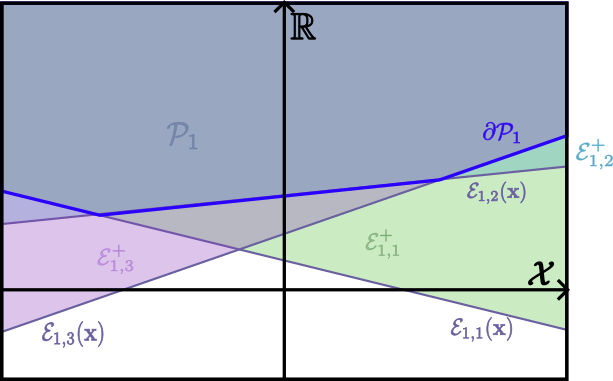
\includegraphics[width=0.75\linewidth]{drawings/max_affine_unit_partition.png}
    \caption{}
    \label{fig:max_affine_unit_partition}
\end{figure}

\begin{lemma}\label{maso_unit_pd}
    The vertical projection on the input space $\mathcal{X}$ of the faces of $\mathcal{P}_i$ from Proposition \ref{prop:image_mas_input_space} construct regions of a power diagram through $$\nu_i(\mathbf{x})=\mathrm{argmax}_{j=1,\dots,r}\mathcal{E}_{i,j}(\mathbf{x}).$$
\end{lemma}

\begin{tproof}
    The faces of $\mathcal{P}_i$ constitute the boundary $\partial\mathcal{P}_i$, which from Proposition \ref{prop:image_mas_input_space} are points $(\mathbf{x},y)$ where $y\geq\mathcal{E}_{i,j}(\mathbf{x})$ for every $j\in\{1,\dots,r\}$ and $y=\mathcal{E}_{i,j^\prime}(\mathbf{x})$ for $j^\prime\in\mathcal{J}\subseteq\{1,\dots,r\}$, where $\mathcal{J}\neq\emptyset$. When $\mathcal{J}=\left\{j^\prime\right\}$, the point $(\mathbf{x},y)$ is an interior point to a face and is vertically projected, through \eqref{eq:maso_unit_operation}, to an interior point of $$\omega_{j^\prime}:=\left\{\mathbf{x}\in\mathcal{X}:\argmax_{j=1,\dots,r}\mathcal{E}_{i,j}(\mathbf{x})=j^\prime\right\}.$$Clearly, the sets $\left\{\omega_1,\dots,\omega_r\right\}$ have disjoint interior, with boundaries between them corresponding to boundaries between faces. Moreover, the set $\left\{\omega_1,\dots,\omega_r\right\}$ cover $\mathcal{X}$ and thus form a power diagram.
\end{tproof}

\begin{theorem}
    The $i^\text{th}$ max-affine unit partitions its input space according to a power diagram with $r$ centroids given by $[\mu]_{i,j}=[A]_{i,j}$ and $[\tau]_{i,j}=2[B]_{i,j}+\left\Vert[A]_{i,j,\cdot}\right\Vert^2$ for all $j\in\{1,\dots,r\}$.
\end{theorem}

\begin{tproof}
    Observe that
    \begin{align*}
        \argmax_{j=1,\dots,r}\left(\mathcal{E}_{i,j}(\mathbf{x})\right)&=\argmax_{j=1,\dots,r}\left(\left\langle[A]_{i,j,\cdot},\mathbf{x}\right\rangle+[B]_{i,j}\right)\\&=\argmax_{j=1,\dots,r}\left(2\left\langle[A]_{i,j,\cdot},\mathbf{x}\right\rangle+2[B]_{i,j}\right)\\&=\argmax_{j=1,\dots,r}\left(\left\Vert[A]_{i,j,\cdot}\right\Vert^2-\left\Vert[A]_{i,j,\cdot}\right\Vert^2+2\left\langle[A]_{i,j,\cdot},\mathbf{x}\right\rangle+\left\Vert\mathbf{x}\right\Vert^2+2[B]_{i,j}\right)\\&=\argmax_{j=1,\dots,r}\left(-\left\Vert[A]_{i,j,\cdot}-\mathbf{x}\right\Vert^2+\left\Vert[A]_{i,j,\cdot}\right\Vert^2+2[B]_{i,j}\right)\\&=\argmin_{j=1,\dots,r}\left(\left\Vert[A]_{i,j,\cdot}-\mathbf{x}\right\Vert^2-\left(\left\Vert[A]_{i,j,\cdot}\right\Vert^2+2[B]_{i,j}\right)\right).
    \end{align*}
    Therefore, we conclude using Lemma \ref{lem:maso_projection_polytope}.
\end{tproof}

\begin{corollary}
    The input space partitioning of a deep network unit is composed of convex polytopes.
\end{corollary}

\section{Max-Affine Spline Operator}

A max-affine spline operator is made by concatenating $k$ max-affine spline units. Let $$\boldsymbol{\nu}(\mathbf{x})=\left(\nu_1(\mathbf{x}),\dots,\nu_k(\mathbf{x})\right)$$and$$E^+_{\boldsymbol{\nu}}=\left\{(\mathbf{x},\mathbf{y})\in\mathcal{X}\times\mathbb{R}^k:[\mathbf{y}]_1\geq\mathcal{E}_{1,\nu_1}(\mathbf{x}),\dots,[\mathbf{y}]_k\geq\mathcal{E}_{1,\nu_k}(\mathbf{x})\right\}.$$

\begin{proposition}\label{prop:image_maso_input_space}
    The layer operator $\mathbf{z}$ maps its input space into the boundary of the $\dim(\mathcal{X})+k$ dimensional convex polytope $\mathbf{P}=\bigcap_{\boldsymbol{\nu}\in\{1,\dots,r\}^k}E_{\boldsymbol{\nu}}^+$ as $$\mathcal{X}\times\mathbf{z}(\mathcal{X})=\mathcal{X}\times [\mathbf{z}]_1(\mathcal{X})\times\dots\times[\mathbf{z}]_k(\mathcal{X})=\partial\mathbf{P}.$$
\end{proposition}

\begin{lemma}\label{lem:maso_projection_polytope}
    The vertical projection on the input space $\mathcal{X}$ of the faces of the polytope of $\mathbf{P}$ from Proposition \ref{prop:image_maso_input_space} construct regions of a power diagram through $\boldsymbol{\nu}$.
\end{lemma}

\begin{theorem}\label{thm:maso_power_diagram}
    A deep network layer partitions its input space according to a power diagram with $\{1,\dots,r\}^k$ cells, centroids $\mu_{\boldsymbol{\nu}}=\sum_{j=1}^k[A]_{j,\nu_j,\cdot}$ and radii $\tau_{\boldsymbol{\nu}}=2\left\langle\mathbf{1},B_{\boldsymbol{\nu}}\right\rangle+\left\Vert\mu_{\boldsymbol{\nu}}\right\Vert^2$.
\end{theorem}

\begin{corollary}
    The input space partitioning of a deep network layer is composed of convex polytopes.
\end{corollary}

\section{Deep Network}

The power diagram partitioning of an $L$-layer deep network can be constructed recursively; each per layer polytope subdivides the previous layer's partitioning.

\newthought{Initialization} identifies the part of the input space of interest $\mathcal{X}^{(0)}\subseteq\mathbb{R}^d$.

\newthought{Layer one} recursion subdivides $\mathcal{X}^{(0)}\subseteq\mathbb{R}^d$ into a power diagram from Theorem \ref{thm:maso_power_diagram} with parameters $A^{(1)}$ and $B^{(1)}$ to obtain $\Omega^{(1)}$.

\newthought{Layer two} recursion subdivides each cell of $\Omega^{(1)}$. Consider the cell $\omega_{\boldsymbol{\nu}^{(1)}}^{(1)}\subseteq\mathbb{R}^d$. Inputs of this cell a projected to $\mathcal{X}^{(1)}\subseteq\mathbb{R}^{d^{(1)}}$ as $$\mathrm{aff}_{\boldsymbol{\nu}^{(1)}}=\left\{A_{\boldsymbol{\nu}^{(1)}}^{(1)}\mathbf{x}+B_{\boldsymbol{\nu}^{(1)}}^{(1)}:\mathbf{x}\in\omega_{\boldsymbol{\nu}^{(1)}}^{(1)}\right\}\subseteq\mathcal{X}^{(1)},$$which is also convex.

\begin{lemma}
    The domain restricted polytope $$\mathbf{P}^{(2)}_{\boldsymbol{\nu}^{(1)}}=\mathbf{P}^{(2)}\cap\left(\mathrm{aff}_{\boldsymbol{\nu}^{(1)}}\times\mathbb{R}^{d^{(2)}}\right),$$where $\mathbf{P}^{(2)}$ is as in Proposition \ref{prop:image_maso_input_space}, can be expressed in the input space $\omega_{\boldsymbol{\nu}^{(1)}}^{(1)}\subseteq\mathcal{X}^{(0)}$ as $$\mathbf{P}_{\boldsymbol{\nu}^{(1)}}^{(1\leftarrow2)}=\bigcap_{\boldsymbol{\nu}^{(2)}}\left\{(\mathbf{x},\mathbf{y})\in\omega_{\boldsymbol{\nu}^{(1)}}^{(1)}\times\mathbb{R}^{d^{(1)}}:[\mathbf{y}]_1\geq\mathcal{E}^{(1\leftarrow 2)}_{1,\nu^{(2)}_1}(\mathbf{x}),\dots,[\mathbf{y}]_{d^{(1)}}\geq\mathcal{E}^{(1\leftarrow 2)}_{d^{(1)},\nu^{(2)}_{d^{(1)}}}(\mathbf{x})\right\},$$with $\mathcal{E}^{(1\leftarrow 2)}_{i,\left[\boldsymbol{\nu}^{(1)}\right]_i}$ the hyperplane with slope $\left(A_{\boldsymbol{\nu}^{(1)}}^{(1)}\right)^\top A_{\mathbf{r}^{(2)}}^{(2)}$ and bias $\left\langle\left[A^{(2)}_{\boldsymbol{\nu}^{(2)}}\right]_{i,j},B_{\boldsymbol{\nu}^{(1)}}\right\rangle+B_{\boldsymbol{\nu}^{(2)}}^{(2)}$ for $j\in\left\{1,\dots,d^{(1)}\right\}$.
\end{lemma}

From Lemma \ref{lem:maso_projection_polytope}, $\mathbf{P}^{(1\leftarrow 2)}_{\boldsymbol{\nu}^{(1)}}$ induces a power diagram on $\omega_{\boldsymbol{\nu}^{(1)}}^{(1)}$, say $\mathrm{PD}^{(1\leftarrow 2)}_{\boldsymbol{\nu}^{(1)}}$ with centroids $$\mu^{(1\leftarrow 2)}_{\boldsymbol{\nu}^{(1)},\boldsymbol{\nu}^{(2)}}=\left(A_{\boldsymbol{\nu}^{(1)}}^{(1)}\right)^\top\mu_{\boldsymbol{\nu}^{(2)}}^{(1\leftarrow 2)}$$ and radii $$\tau_{\boldsymbol{\nu}^{(1)},\boldsymbol{\nu}^{(2)}}^{(1\leftarrow 2)}=\left\Vert\mu_{\boldsymbol{\nu}^{(1)},\boldsymbol{\nu}^{(2)}}^{(1\leftarrow 2)}\right\Vert^2+2\left\langle\mu_{\boldsymbol{\nu}^{(2)}}^{(2)},B_{\boldsymbol{\nu}^{(1)}}^{(1)}\right\rangle+2\left\langle\mathbf{1},B_{\boldsymbol{\nu}^{(2)}}^{(2)}\right\rangle$$for every $\boldsymbol{\nu}^{(2)}\in\{1,\dots,r\}^{d^{(2)}}$. Repeating this for every cell of $\Omega^{(1)}$ leads to $$\Omega^{(1,2)}=\bigcup_{\boldsymbol{\nu}^{(1)}}\mathrm{PD}^{(1\leftarrow 2)}_{\boldsymbol{\nu}^{(1)}}.$$

\begin{figure}
    \centering
    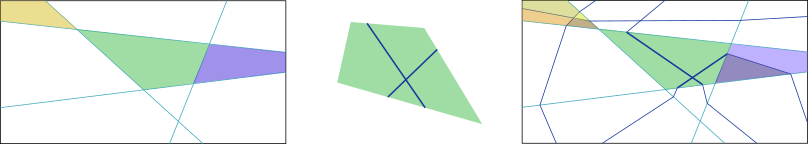
\includegraphics[width=\linewidth]{drawings/iterative_partitioning_procedure.png}
    \caption{\textbf{Left:} The bounding box represents $\mathcal{X}^{(0)}$, with each line representing the partition boundary induced by a unit of layer one. A few regions of $\Omega^{(1)}$ are highlighted, suppose that the green region corresponds to $\omega_{\boldsymbol{v}^{(1)}}^{(1)}$. \textbf{Centre:} Represents $\mathrm{aff}_{\boldsymbol{v}^{(1)}}$ with the blue lines representing the power diagram induces by the vertical projection of $\mathbf{P}^{(2)}_{\boldsymbol{v}^{(1)}}$. \textbf{Right:} Represents the power diagram $\mathrm{PD}^{(1\leftarrow 2)}_{\boldsymbol{v}^{(1)}}$ along with the other power diagrams for the other cells of $\Omega^{(1)}$. Altogether they constitute $\Omega^{(1,2)}$.}
    \label{fig:iterative_partitioning_procedure}
\end{figure}

\newthought{Layer $\ell$} recursion subdivides each cell of $\Omega^{(1,\dots,\ell-1)}$ from the previous recursion steps, forming the power diagram $$\Omega^{(1,\dots,\ell)}=\bigcup_{\boldsymbol{\nu}^{(1\leftarrow\ell-1)}}\mathrm{PD}_{\boldsymbol{\nu}^{(1\leftarrow\ell-1)}}.$$

\begin{theorem}
    Each cell $\omega_{\boldsymbol{\nu}^{(1\leftarrow\ell-1}}^{(1\leftarrow\ell-1)}\in\Omega^{(1\leftarrow\ell-1)}$ is subdivided into $\mathrm{PD}^{(1\leftarrow\ell)}_{\boldsymbol{\nu}^{(1\leftarrow\ell-1)}}$, a power diagram with domain $\omega_{\boldsymbol{\nu}^{(1\leftarrow\ell-1)}}^{(1\leftarrow\ell-1)}\in\Omega^{(1\leftarrow\ell-1)}$, centroids $$\mu_{\boldsymbol{\nu}^{(1\leftarrow\ell)}}^{(1\leftarrow\ell)}=\left(A_{\boldsymbol{\nu}^{(1\leftarrow\ell-1)}}^{(1\leftarrow\ell-1)}\right)^\top\mu_{\boldsymbol{\nu}^{(\ell)}}^{(\ell)}$$and radii $$\tau_{\boldsymbol{\nu}^{(1\leftarrow\ell)}}^{(1\leftarrow\ell)}=-\left\Vert\mu_{\boldsymbol{\nu}^{(1\leftarrow\ell)}}^{(1\leftarrow\ell)}\right\Vert^2-2\left\langle\mu_{\boldsymbol{\nu}^{(\ell)}}^{(\ell)},B_{\boldsymbol{\nu}^{(1\leftarrow\ell-1)}}^{(1\leftarrow\ell-1)}\right\rangle-2\left\langle\mathbf{1},B_{\boldsymbol{\nu}^{(\ell)}}^{(\ell)}\right\rangle,$$for every $\boldsymbol{\nu}^{(i)}\in\{1,\dots,r\}^{d^{(i)}}$ with $$B^{(1\leftarrow\ell-1)}=\sum_{\ell^\prime=1}^{\ell-1}\left(\prod_{i=\ell-1}^{\ell^\prime}A_{\boldsymbol{\nu}^{(i)}}^{(i)}\right)B_{\boldsymbol{\nu}^{\left(\ell^\prime\right)}}^{\left(\ell^\prime\right)}$$forming $\Omega^{(1\leftarrow\ell)}$.
\end{theorem}

\begin{corollary}\label{cor:deep_network_layer_convex_polytopes}
    The input space partitioning of a deep network is composed of convex polygons.
\end{corollary}

\section{Decision Boundary}

Consider the case of $r=2$ nonlinear activation operators. 

\begin{definition}
    The edges of a polytope $\mathcal{P}_i^{(\ell)}$ in a space $\mathcal{X}^{\left(\ell^\prime\right)}$, for $\ell^\prime<\ell$, are $$\mathrm{edge}_{\mathcal{X}^{\left(\ell^\prime\right)}}(i,\ell)=\left\{\mathbf{x}\in\mathcal{X}^{\left(\ell^\prime\right)}:\mathcal{E}_{i,2}^{(\ell-1)}\left(\mathbf{z}^{\left(\ell^\prime\to\ell-1\right)}(\mathbf{x})\right)=0\right\},$$where $\mathbf{z}^{\left(\ell^\prime\to\ell-1\right)}=\mathbf{z}^{(\ell-1)}\circ\dots\circ\mathbf{z}^{\left(\ell^\prime\right)}$.\footnote{Note how it is sufficient to only consider $\mathcal{E}_{i,2}^{(\ell-1)}$, due our construction Example \ref{eg:maso_activation_operators}, the piecewise continuity of the operators and the fact that $r=2$.}
\end{definition}

That is, edges are the level set curve of the unit in $\mathcal{X}^{\left(\ell^\prime\right)}$. Let $$\mathrm{Pol}^{(\ell)}(\mathbf{x})=\prod_{i=1}^{d^{(\ell)}}\left(\left[\mathbf{z}^{(\ell)}\right]_i\circ\mathbf{z}^{(\ell-1)}\circ\dots\circ\mathbf{z}^{(1)}\right)(\mathbf{x}).$$

\begin{theorem}
    The polynomial $\mathrm{Pol}^{(\ell)}$ is of order $\prod_{\ell^\prime=1}^{\ell}d^{\left(\ell^\prime\right)}$, with roots corresponding to the partitioning boundaries $$\partial\Omega^{(1\leftarrow\ell)}=\bigcup_{\ell^\prime=1}^{\ell}\bigcup_{i=1}^{d^{\left(\ell^\prime\right)}}\mathrm{edge}_{\mathcal{X}^{(0)}}\left(i,\ell^\prime\right)=\left\{\mathbf{x}\in\mathcal{X}^{(0)}:\prod_{\ell^\prime=1}^{\ell}\mathrm{Pol}^{\left(\ell^\prime\right)}(\mathbf{x})=0\right\}.$$In particular, the root order gives the dimension of the boundary.
\end{theorem}

\begin{corollary}
    The decision boundary of an $L$ layer deep network with $d^{(L)}=1$ is the edge of the last layer polytope $\mathbf{P}^{(L)}$ expressed in $\mathcal{X}^{(0)}$. Namely, $$\mathrm{DB}=\left\{\mathbf{x}\in\mathcal{X}^0:f(\mathbf{x})=0\right\}=\mathrm{edge}_{\mathcal{X}^{(0)}}(1,L)\subseteq\partial\Omega^{(1,\dots,L)}.$$
\end{corollary}

\section{References}

Results in Chapter \ref{ch:partition_geometry} from \citet{balestrieroGeometryDeepNetworks2019}.

\chapter{Initialisation and Regularisation}

\section{Introduction}

Having developed an understanding of how the parameters of a deep network effect the underlying geometry of the deep network, we can start investigating the precise effects of operators on the functional geometry of a deep network and how this translates into properties of the deep network. Specifically, we focus on the normalisation operations and how they initialise and regularise deep networks.

\section{Batch Normalisation}\label{sec:batch_norm}

For a batch normalised layer, let $$\left[\mathbf{h}^{(\ell)}\right]_i=\frac{\left\langle\left[W^{(\ell)}\right]_{i,\cdot},\mathbf{z}^{(\ell-1)}\right\rangle-\left[\mu^{(\ell)}\right]_i}{\left[\sigma^{(\ell)}\right]_i},$$so that $\mathbf{h}^{(\ell)}$ is the pre-activation\footnote{This is well-defined provided $\left\Vert\left[W^{(\ell)}\right]_{i,\cdot}\right\Vert_2^2>0$ and the inputs of the batch are not orthogonal to $\left[W^{(\ell)}\right]_{i,\cdot}$.} of layer $\ell$ and $\mathbf{z}^{(\ell)}=\sigma_{\text{act}}\left(\mathbf{h}^{(\ell)}\right)$.

The separation of regimes induced by the affine components of $\sigma_{\text{act}}$\footnote{In this analysis we are assuming that $\sigma_{\text{act}}$ consists of two affined components joining at the origin.} is governed by the hyperplane arrangement $$\partial\Omega^{(\ell)}=\bigcup_{i=1}^{d^{(\ell)}}\mathcal{H}^{(\ell)}_i$$where $$\mathcal{H}^{(\ell)}_i=\left\{\mathbf{z}^{(\ell-1)}\in\mathbb{R}^{d^{(\ell-1)}}:\left[\mathbf{h}^{(\ell)}\right]_i=0\right\}$$is a $d^{(\ell)}$-dimensional hyperplane.\footnote{Note that $\mathcal{H}^{(\ell)}_i$ is independent of $\left[\sigma^{(\ell)}\right]_i$.}

\subsection{Single Layer Analysis}\label{subsec:single_layer_analysis}

\begin{lemma}\label{lem:distance_to_hyperplane}
    The Euclidean distance from a point $\mathbf{v}$ in layer $\ell$'s input space and $\mathcal{H}^{(\ell)}_i$ is $$d\left(\mathbf{v},\mathcal{H}^{(\ell)}_i\right)=\frac{\left\vert\left\langle\left[W^{(\ell)}\right]_{i,\cdot},\mathbf{v}\right\rangle-\left[\mu^{(\ell)}\right]_i\right\vert}{\left\Vert\left[W^{(\ell)}\right]_{i,\cdot}\right\Vert_2},$$when $\left\Vert\left[W^{(\ell)}\right]_{i,\cdot}\right\Vert_2>0$.\footnote{For a proof refer to \citet{alexanderschrijverTheoryLinearInteger1998}.}
\end{lemma}

Let $\mathcal{V}$ be a collection of points in $\ell$'s input space. From Lemma \ref{lem:distance_to_hyperplane}, it follows that the unit least squares distance is 
\begin{equation}\label{eq:unit_least_squares}
    \mathcal{L}_i\left(\left[\mu^{(\ell)}\right]_i;\mathcal{V}\right)=\frac{1}{\vert\mathcal{V}\vert}\sum_{\mathbf{v}\in\mathcal{V}}d\left(\mathbf{v},\mathcal{H}^{(\ell)}_i\right)^2:=\frac{\left[\sigma^{(\ell)}\right]_{\ell,i}}{\left\Vert\left[W^{(\ell)}\right]_{i,\cdot}\right\Vert_2^2}
\end{equation}
for $i=1,\dots,d^{(\ell)}$ where the total least squares distance is $$\mathcal{L}\left(\mu^{(\ell)};\mathcal{V}\right)=\sum_{i=1}^{d^{(\ell)}}\mathcal{L}_i\left(\left[\mu^{(\ell)}\right]_i;\mathcal{V}\right).$$

\begin{theorem}\label{thm:minimising_tls}
    Consider a deep network layer $\ell$ equipped with batch normalisation. Let $\mathcal{B}^{(\ell)}\subseteq\mathcal{X}^{(\ell)}$ be a mini-batch. Then $\mu^{(\ell)}$ as given by \eqref{eq:bn_parameters} is the unique minimiser of $\mathcal{L}\left(\mu^{(\ell)};\mathcal{B}^{(\ell)}\right)$.
\end{theorem}

\begin{tproof}
    Consider the optimisation problem $$\min_{\mu\in\mathbb{R}^{d^{(\ell)}}}\mathcal{L}\left(\mu;\mathcal{Z}\right).$$Since the problem is unconstrained and the sum is separable, we can focus on $[\mu]_i$, yielding the optimisation problem $$\min_{[\mu]_i\in\mathbb{R}}\sum_{\mathbf{z}\in\mathcal{Z}}\frac{\left\vert\left\langle\left[W^{(\ell)}\right]_{i,\cdot},\mathbf{z}\right\rangle-[\mu]_i\right\vert^2}{\left\Vert\left[W^{(\ell)}\right]_{i,\cdot}\right\Vert_2^2}.$$Observe that, 
    \begin{align*}
        \partial\left(\sum_{\mathbf{z}\in\mathcal{Z}}\frac{\left\vert\left\langle\left[W^{(\ell)}\right]_{i,\cdot},\mathbf{z}\right\rangle-[\mu]_i\right\vert^2}{\left\Vert\left[W^{(\ell)}\right]_{i,\cdot}\right\Vert_2^2}\right)&=-2\sum_{\mathbf{z}\in\mathcal{Z}}\frac{\left\langle\left[W^{(\ell)}\right]_{i,\cdot},\mathbf{z}\right\rangle}{\left\Vert\left[W^{(\ell)}\right]_{i,\cdot}\right\Vert_2^2}\\&\quad+2\vert\mathcal{Z}\vert\frac{[\mu]_i}{\left\Vert\left[W^{(\ell)}\right]_{i,\cdot}\right\Vert_2^2}.
    \end{align*}
    It follows that the first derivative is zero if and only if $$[\mu]_i=\frac{1}{\vert\mathcal{Z}\vert}\sum_{\mathbf{z}\in\mathcal{Z}}\left\langle\left[W^{(\ell)}\right]_{i,\cdot},\mathbf{z}\right\rangle.$$Second derivative calculations confirm that this turning point is a minimum. By aggregating these across each of the $d^{(\ell)}$ dimensions, we deduce the desired result.
\end{tproof}

\begin{remark}
    For concreteness we note that by taking $\mathcal{B}^{(\ell)}=\mathcal{X}^{(\ell)}$ in Theorem \ref{thm:minimising_tls} we deduce that $\bar{\mu}^{(\ell)}$ is the unique minimiser of $\mathcal{L}\left(\mu^{(\ell)};\mathcal{X}^{(\ell)}\right)$.
\end{remark}

\begin{definition}
    A collection of hyperplanes $\mathcal{H}$ is central if $$\bigcap_{H\in\mathcal{H}}H\neq\emptyset.$$
\end{definition}

\begin{corollary}
    On $\mathcal{Z}\subseteq\mathcal{X}$, the induced arrangement of hyperplanes $\partial\Omega^{(\ell)}$ is central.
\end{corollary}

\begin{tproof}
    Let $\bar{\mathbf{z}}$ be the centroid of $\mathcal{Z}$. For $i\in\left\{1,\dots,d^{(\ell)}\right\}$ observe that
    \begin{align*}
        \left\langle\left[W^{(\ell)}\right]_{i,\cdot},\bar{\mathbf{z}}\right\rangle&=\left\langle\left[W^{(\ell)}\right]_{i,\cdot},\frac{1}{\vert\mathcal{Z}\vert}\sum_{\mathbf{z}\in\mathcal{Z}}\mathbf{z}\right\rangle\\&=\frac{1}{\vert\mathcal{Z}\vert}\sum_{\mathbf{z}\in\mathcal{Z}}\left\langle\left[W^{(\ell)}\right]_{i,\cdot},\mathbf{z}\right\rangle\\&\overset{\eqref{eq:bn_parameters}}{=}\left[\mu^{(\ell)}\right]_i.
    \end{align*}
    Therefore, $\bar{\mathbf{z}}\in\mathcal{H}^{(\ell)}_i$. Since, $i$ was arbitrary it follows that $$\bar{\mathbf{z}}\in\bigcap_{i=1}^{d^{(\ell)}}\mathcal{H}^{(\ell)}_i,$$meaning the arrangement $\partial\Omega^{(\ell)}$ is central.
\end{tproof}

In this analysis, we see that $\mu^{(\ell)}$ has a direct influence on the partitioning of a deep network layer's input space. The effect of the parameter $\sigma^{(\ell)}$ are introduced when composing deep network layers.

\subsection{Multilayer Analysis}

Similarly to Section \ref{subsec:single_layer_analysis}, we have $$\partial\Omega^{(1,\dots,\ell)}=\bigcup_{j=1}^{\ell}\bigcup_{i=1}^{d^{(j)}}\left\{\mathbf{x}\in\mathbb{R}^{d^{(1)}}:\left[\mathbf{h}^{(j)}\right]_i=0\right\}=:\bigcup_{j=1}^{\ell}\bigcup_{i=1}^{d^{(j)}}\mathcal{F}^{(j)}_{i,\omega}.$$In this scenario, the hyperplanes $\mathcal{H}^{(j)}_i$ are folded through the preceding layers to form facets $$\mathcal{F}^{(j)}_{i,\omega}=\left\{\mathbf{x}\in\omega:\left[\mathbf{h}^{(j)}\right]_i=0\right\}$$for $\omega\in\Omega^{(1,\dots,j)}$.\footnote{We can characterise the facets using the regions of $\Omega^{(1,\dots,j)}$, since the folds only happen at the boundaries of these regions as within the regions the transformation is affine.}With $\mathcal{F}^{(j)}_{i}:=\bigcup_{\omega\in\Omega^{(1,\dots,j)}}\mathcal{F}^{(j)}_{i,\omega}$ we can write $$\partial\Omega^{(1,\dots,\ell)}=\bigcup_{j=1}^{\ell}\bigcup_{i=1}^{d^{(j)}}\mathcal{F}^{(j)}_{i}.$$

\paragraph{The Effect of $\mu^{(\ell)}$.}

\begin{theorem}\label{thm:effect_mean_bn_multilayer}
    Consider a deep network layer $\ell>1$ equipped with batch normalisation. Suppose that layers $1,\dots,\ell-1$ have fixed batch normalisation parameters. Let $\mu^{(\ell)}$ and $\tilde{\mu}^{(\ell)}$ yield hyperplanes $\mathcal{H}^{(\ell)}_i$ and $\tilde{\mathcal{H}}^{(\ell)}_i$ which are folded into $\mathcal{F}^{(\ell)}_i$ and $\tilde{\mathcal{F}}^{(\ell)}_i$ respectively. Then, $d\left(\mathbf{z}^{(\ell)}(\mathbf{x}),\mathcal{H}^{(\ell)}_i\right)<d\left(\mathbf{z}^{(\ell)}(\mathbf{x}),\tilde{\mathcal{H}}^{(\ell)}_i\right)$ implies that $d\left(\mathbf{x},\mathcal{F}^{(\ell)}_i\right)<d\left(\mathbf{x},\tilde{\mathcal{F}}^{(\ell)}_i\right)$.\footnote{Here, $d\left(\mathbf{x},\mathcal{F}^{(\ell)}_{i}\right)=\min_{\mathbf{x}^\prime\in\mathcal{F}^{(\ell)}_{i}}\left\Vert\mathbf{x}-\mathbf{x}^\prime\right\Vert^2$.}
\end{theorem}

\begin{tproof}
    Let $$\mathbf{x}^*=\argmin_{\mathbf{u}\in\mathcal{F}_{\ell,i}}\left\Vert\mathbf{x}-\mathbf{u}\right\Vert_2.$$Let $l:[0,1]\to\mathbb{R}^d$ be given by $$l(\theta)=\mathbf{x}^*\theta+(1-\theta)\mathbf{x}.$$In the input space of layer $\ell$, the line $l$ becomes the piecewise affine parametric line $$\mathbf{z}^{(\ell-1)}(\theta)=\left(f_{\ell-1}\circ\dots\circ f_1\right)(l(\theta)).$$Now if there exists $\theta^\prime<1$ such that $\mathbf{z}^{(\ell-1)}\left(\theta^\prime\right)\in\mathcal{H}^{(\ell)}_i$ then there exists $\theta<1$ such that $l(\theta)\in\mathcal{F}^{(\ell)}_i$, Figure \ref{fig:multilayer_analysis_batchnorm_proof}.
    \begin{figure}
        \centering
        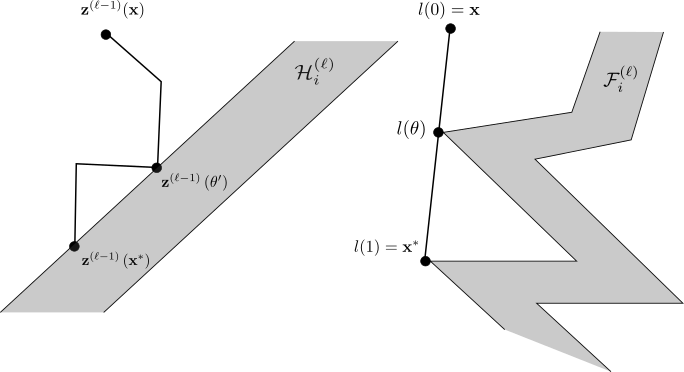
\includegraphics[width=0.75\linewidth]{drawings/multilayer_analysis_batchnorm_proof.png}
        \caption{}
        \label{fig:multilayer_analysis_batchnorm_proof}
    \end{figure}
    In other words, if the hyperplane $\mathcal{H}^{(\ell)}_i$ is bought closer to $\mathbf{z}^{(\ell-1)}(\mathbf{x})$ within the input space of layer $\ell$, then $\mathcal{F}^{(\ell)}_i$ is bought closer to $\mathbf{x}$. 
\end{tproof}

That is, translating hyperplanes closer to $\mathbf{z}^{(\ell)}$ in the input space of layer $\ell$, moves the folded hyperplane closer to $\mathbf{x}$ in the input space of the deep network.

\begin{corollary}
    Consider the setting of Theorem \ref{thm:effect_mean_bn_multilayer}. Then $\mathbf{z}^{(\ell)}(\mathbf{x})$ lies on the hyperplane $\mathcal{H}^{(\ell)}_i$ for some $i$ if and only if $\mathbf{x}$ lies on the corresponding folder hyperplane $\mathcal{F}^{(\ell)}_i$ in the input space of the deep network.
\end{corollary}

\paragraph{The Effect of $\sigma^{(\ell)}$.}

The parameter $\sigma^{(\ell)}$ optimises the dihedral angles between adjacent facets of the folded hyperplanes, to direct them toward the training data. For an input $\mathbf{z}$, let $Q^{(\ell)}$ be the square diagonal matrix with entries $$\left[Q^{(\ell)}\right]_{i,i}=\begin{cases}\frac{\alpha}{\left[\sigma^{(\ell)}\right]_i}&\left[\mathbf{h}^{(\ell)}\right]_i<0\\\frac{1}{\left[\sigma^{(\ell)}\right]_i}&\left[\mathbf{h}^{(\ell)}\right]_i\geq0,\end{cases}$$where $\mathbf{h}^{(\ell)}$ is the pre-activation of $\mathbf{z}$, and $\alpha$ is a parameter dependent on the activation function operating on layer $\ell$.\footnote{For ReLU we set $\alpha=0$, for leaky ReLU we set $\alpha=-1$, for absolute value we set $\alpha=-1$.}

The matrix $Q^{(\ell)}$ is constant across each region $\omega\in\Omega^{(\ell)}$. We will note this dependency with $Q^{(\ell)}(\omega)$.

\begin{theorem}\label{thm:effect_std_bn_multilayer}
    Consider a two-layer batch normalised equipped deep network employing a leaky-ReLU or absolute value activation function. Let $\omega,\omega^\prime\in\Omega$ be adjacent regions whose boundaries contain the facets $\mathcal{F}_{2,i,\omega}$ and $\mathcal{F}_{2,i,\omega^\prime}$, which are created from folding across the shared hyperplane boundary $\mathcal{H}^{(1)}_i$. The dihedral angles between these hyperplanes are $$\begin{cases}\theta\left(\mathcal{F}^{(2)}_{i,\omega},\mathcal{H}^{(1)}_j\right)=\arccos\left(\frac{\left\vert\left[W^{(2)}\right]_{i,\cdot}^\top Q^{(1)}(\omega)W^{(1)}\left[W^{(1)}\right]_{j,\cdot}\right\vert}{\left\Vert\left[W^{(2)}\right]_{i,\cdot}^\top Q^{(1)}(\omega)W^{(1)}\right\Vert\left\Vert\left[W^{(1)}\right]_{j,\cdot}\right\Vert}\right)\\\theta\left(\mathcal{F}^{(2)}_{i,\omega^\prime},\mathcal{H}^{(1)}_j\right)=\arccos\left(\frac{\left\vert\left[W^{(2)}\right]_{i,\cdot}^\top Q^{(1)}(\omega^\prime)W^{(1)}\left[W^{(1)}\right]_{j,\cdot}\right\vert}{\left\Vert\left[W^{(2)}\right]_{i,\cdot}^\top Q^{(1)}\left(\omega^\prime\right)W^{(1)}\right\Vert\left\Vert\left[W^{(1)}\right]_{j,\cdot}\right\Vert}\right)\\\theta\left(\mathcal{F}^{(2)}_{i,\omega},\mathcal{F}^{(2)}_{i,\omega^\prime}\right)=\arccos\left(\frac{\left\vert\left[W^{(2)}\right]_{i,\cdot}^\top Q^{(1)}(\omega)W^{(1)}\left(W^{(1)}\right)^\top Q^{(1)}\left(\omega^\prime\right)\left[W^{(2)}\right]_{i,\cdot}\right\vert}{\left\Vert\left[W^{(2)}\right]_{i,\cdot}^\top Q^{(1)}(\omega)W^{(1)}\right\Vert\left\Vert\left[W^{(2)}\right]_{i,\cdot}^\top Q^{(1)}\left(\omega^\prime\right)W^{(1)}\right\Vert}\right).\end{cases}$$
\end{theorem}

\begin{remark}
    Note that $Q^{(1)}(\omega)$ and $Q^{(1)}\left(\omega^\prime\right)$ differ only in the $(i,i)$ entry where one takes the value $\frac{1}{\left[\sigma^{(1)}\right]}$ and the other $\frac{\alpha}{\left[\sigma^{(1)}\right]}$. Furthermore, recall that from \eqref{eq:unit_least_squares} we have $\left[\sigma^{(\ell)}\right]_i^2\propto\min_{\mu^{(\ell)},i}\mathcal{L}\left(\left[\mu^{(\ell)}\right]_i;\mathcal{B}^{(\ell)}\right)$. Therefore, using Theorem \ref{thm:effect_std_bn_multilayer} we yield the following insights.
    \begin{itemize}
        \item If $\mathcal{H}^{(1)}_i$ is well-aligned with the training data $\mathcal{B}^{(1)}$, then the total least squares error, and hence $\left[\sigma^{(1)}\right]_i^2$, will be small. For the absolute value activation function it follows that $\theta\left(\mathcal{F}^{(2)}_{i,\omega},\mathcal{H}^{(1)}_i\right)\approx0$ and $\theta\left(\mathcal{F}^{(2)}_{i,\omega^\prime},\mathcal{H}^{(1)}_i\right)\approx0$, meaning $\mathcal{F}^{(2)}_{i,\omega}$ and $\mathcal{F}^{(2)}_{i,\omega^\prime}$ are folded to closely align with $\mathcal{H}^{(1)}_i$ and thus the data.
        \item If $\mathcal{H}^{(1)}_i$ is not well-aligned with the training data $\mathcal{B}^{(1)}$, then the total least squares error, and hence $\left[\sigma^{(1)}\right]_i^2$, will be large. Forcing $Q^{(1)}(\omega)\approx Q^{(1)}\left(\omega^\prime\right)$, making $\theta\left(\mathcal{F}^{(2)}_{i,\omega},\mathcal{F}^{(2)}_{i,\omega^\prime}\right)\approx\pi$, meaning that $\mathcal{H}^{(1)}_i$ will not appreciably fold intersection the layer two facets.
    \end{itemize}
\end{remark}

\subsection{Initialization Scheme}

In the case of binary classification, we can concretely intuit on the effect of batch normalisation.

\begin{proposition}\label{prop:initialisation_bn_binary_classification}
    Consider a $L$-layer deep network configured as a binary classifier on training data $\mathcal{X}$ using a leaky ReLU activation function at each layer, arbitrary weights $W^{(\ell)}$ at each layer, batch normalisation at layers $\ell=1,\dots,L-1$, and layer $L$ an affine layer with zero bias. Then for any training mini-batch from $\mathcal{X}$, there will be at least one data point on either side of the decision boundary.
\end{proposition}

\begin{tproof}
    Each mini-batch input to the last layer will have one input whose entries contain positive and negative values. Hence each dimension will have at least one negative value with the other being positive, or vice-versa. Since the last layer has zero bias, the decision boundary is the hyperplanes of zero level sets of each output unit. Since being on one side of the decision boundary in the deep network's input space is equivalent to being on one side of the linear decision boundary in the last layer's input space, there has to be at least one sample on one side of the decision boundary compared to the other samples.
\end{tproof}

In the setting of Proposition \ref{prop:initialisation_bn_binary_classification}, batch normalisation primes learning through stochastic gradient descent by ensuring the decision boundary passes through every mini-batch.

\subsection{Jitter}

The parameters $\mu^{(\ell)}$ and $\sigma^{(\ell)}$ can be thought of as stochastic estimators to $\bar{\mu}^{(\ell)}$ and $\bar{\sigma}^{(\ell)}$ respectively.

\begin{proposition}\label{prop:jitter_bn}
    Consider layer $\ell>1$ of a batch normalised deep network. Assume that inputs $\mathbf{z}^{(\ell-1)}$ are independent and identically distributed, with the distribution having zero mean and covariance matrix $\mathrm{diag}(\mathbf{m}\rho)$. Then $$\mathrm{var}\left(\left[\mu^{(\ell)}\right]_i\right)=\frac{\left\langle\left[W^{(\ell)}\right]_{i,\cdot}^2,\mathbf{m}\rho\right\rangle}{\left\vert\mathcal{B}^{(\ell)}\right\vert}$$and$$\mathrm{var}\left(\left[\sigma^{(\ell)}\right]_i^2\right)=\frac{1}{\left\vert\mathcal{B}^{(\ell)}\right\vert}\left(\left[\phi^{(\ell)}\right]_i-\frac{\left\langle\left[W^{(\ell)}\right]_i^2,\mathbf{m}\rho\right\rangle\left(\left\vert\mathcal{B}^{(\ell)}\right\vert-3\right)}{\left\vert\mathcal{B}^{(\ell)}\right\vert-1}\right),$$where $\left[W^{(\ell)}\right]_i^2$ is coordinate-wise and $\left[\phi^{(\ell)}\right]_i$ is the fourth-order central moment of $\left\langle\left[W^{(\ell)}\right]_i,\mathbf{z}^{(\ell)}\right\rangle$.
\end{proposition}

Proposition \ref{prop:jitter_bn} formalises the intuition that batch normalisation introduces noise into the learning process. 

\section{Layer Normalisation}

\section{References}

Section \ref{sec:batch_norm} from \citet{balestrieroBatchNormalizationExplained2022}.

\chapter{Optimization}

\section{Introduction}

In this chapter we seek to understand how the learning process of deep networks effects the functional geometry of the deep network.

\chapter{Data Distribution}

\section{Introduction}

From previous chapters, we have developed a sense of how the training data of a deep network can influence its underlying functional geometry, either through normalisation operators or the optimization procedure. In this chapter we aim to develop this question further by exploring what can be inferred about the data distribution of a training set from the geometry of the deep network. More specifically, we investigate the geometries necessary for capturing certain distributional features in a training set.

\part{The Practical Implications}

\chapter{Visualisation}\label{ch:visualisation}

\section{Introduction}

In this chapter we develop the necessary results to construct methods for exactly computing visualisations of a deep network's geometry. Ultimately, we arrive at a computational algorithm for exactly depicting the induced partition of a deep network on a two-dimensional slice of its input domain.  

\section{Exact Computation of Partition Boundaries}

Throughout these sections we are assuming that the piecewise affine non-linearity of the deep network is either ReLU, leaky ReLU or absolute value. 

Recall Proposition \ref{prop:expanding_dn_parameters_with_layer_parameters}, Proposition \ref{prop:characterising_region_maps_relu_deep_networks}, and the notation outlined in statement 3 of Remark \ref{rem:characterising_region_maps_relu_deep_networks}, so that for a deep network $f$ we have $A_{\omega}^{(\ell)}$ and $b^{(\ell)}$ as 
\begin{equation}\label{eq:mapping_on_regions_using_gradients}
    \begin{cases}
        A_{\omega}^{(1\leftarrow\ell)}=\prod_{i=1}^{\ell}Q^{(i)}[\omega]W^{(i)}\\b_{\omega}^{(1\leftarrow\ell)}=Q^{(\ell)}[\omega]b^{(\ell)}+\sum_{i=1}^{\ell-1}\left(\prod_{j=i+1}^{\ell}Q^{(j)}[\omega]W^{(j)}\right)Q^{(i)}[\omega]b^{(i)},
    \end{cases}
\end{equation}
where $q_{\omega}^{(\ell)}$, in this setting, is the point-wise derivative of $\sigma$ at the pre-activation $W^{(\ell)}\mathbf{z}^{(\ell-1)}+b^{(\ell)}$ for $\omega\in\Omega$.

Furthermore, recall that at layer $\ell$ of a deep network, we let $$\mathcal{H}^{(\ell)}_i=\left\{\mathbf{z}^{(\ell-1)}\in\mathbb{R}^{d^{(\ell-1)}}:\left\langle[W^{(\ell)}]_{i,\cdot},\mathbf{z}^{(\ell-1)}\right\rangle+\left[b^{(\ell)}\right]_i=0\right\}.$$

\begin{lemma}\label{lem:projection_hyperplane_to_input_space}
    The hyperplane $\mathcal{H}^{(\ell)}_i\subseteq\mathbb{R}^{d^{(\ell-1)}}$ can be projected onto the tangent space of a region $\omega\in\Omega\subseteq\mathbb{R}^d$ as $$\mathrm{proj}_{\omega}\left(\mathcal{H}^{(\ell)}_i\right)=\left\{\mathbf{x}\in\mathbb{R}^d:\left\langle\left[W^{(\ell)}\right]_{i,\cdot},A^{(\ell-1)}_{\omega}\mathbf{x}+b^{(\ell-1)}_{\omega}\right\rangle+\left[b^{(\ell)}\right]_i=0\right\}$$
\end{lemma}

\begin{tproof}
    This follows as $$\mathbf{z}^{(\ell-1)}=A^{(\ell-1)}_{\omega}\mathbf{x}+b^{(\ell-1)}_{\omega}$$ for $\mathbf{x}\in\omega$.
\end{tproof}

\begin{theorem}
    Consider a binary classification deep network, that is $d^{(L)}=1$. In $\mathbb{R}^{d^{(L-1)}}$, the decision boundary is the hyperplane $\mathcal{H}^{(L)}_i$. Therefore, in $\mathbb{R}^d$ the decision boundary is $$\bigcup_{\omega\in\Omega}\mathrm{proj}_{\omega}\left(\mathcal{H}^{(L)}_i\right)\cap\omega.$$
\end{theorem}

\begin{tproof}
    This follows by applying Lemma \ref{lem:projection_hyperplane_to_input_space} to each $\omega\in\Omega$.
\end{tproof}

\section{SplineCam}\label{sec:splinecam}

SplineCam is an algorithm to perform that exact computation of the partition boundary of a deep network on two-dimensional subspaces of the input space.

Recall that $\Omega^{(1\leftarrow\ell)}$ is the partition of the input space induced by the layers $1,\dots,\ell$ of a deep network. The SplineCam constitutes Algorithm \ref{alg:partitions} and Algorithm \ref{alg:cycles}, and can be summarised as follows.
\begin{itemize}
    \item Determine a two-polytope subspace $P\subseteq\mathbb{R}^d$.
    \item Using Algorithm \ref{alg:partitions}, partition $P$ into $\Omega^{(1)}$ using the hyperplanes $\mathcal{H}^{(1)}_i$.
    \item For each $\omega\in\Omega^{(1)}$, use Lemma \ref{eq:mapping_on_regions_using_gradients} and then Lemma \ref{lem:projection_hyperplane_to_input_space} to obtain $\mathrm{proj}_{\omega}\left(\mathcal{H}^{(2)}_i\right)$.
    \item Using Algorithm \ref{alg:partitions}, partition each $\omega\in\Omega^{(1)}$ through the hyperplanes $\mathrm{proj}_{\omega}\left(\mathcal{H}^{(2)}_i\right)$ to arrive at $\Omega^{(1\leftarrow2)}$.
    \item Repeat for all layers up to $\ell=L$ to obtain the final partition.
\end{itemize}

\begin{algorithm}
\caption{Find the partitions of a two-polytope induced by the hyperplanes $\mathcal{H}$.}\label{alg:partitions}
\begin{algorithmic}
\Require $P$, $\mathcal{H}$.
\State Solve for $$N=\left\{H_i\cap\left(H_j\cup P_e\right):H_i,H_j\in\mathcal{H}\text{ with }i\neq j\right\},$$where $P_e$ are the edges of $P$.
\State For each $H_i$, sort $N$ and connect in a sequence to obtain edges $E$.
\State Obtain set of cycles $C$ from the undirected graph $G=(E,N)$ using Algorithm \ref{alg:cycles}.
\end{algorithmic}
\end{algorithm}

\begin{algorithm}
\caption{Compute the cycles in an undirected graph $G=(E,N)$.}\label{alg:cycles}
\begin{algorithmic}
\Require $G=(E,N)$, $P_e\subseteq E$, $e_s\subseteq P_e$.
\State Initialise $C=\emptyset$ and $E_q=\emptyset$.
\State $G^\prime\leftarrow\text{bidirectional}(G)$.
\State Append $e_s$ to $E_q$.
\State Remove $e_s$ from $G^\prime$.
\While{$E_q\neq\emptyset$}
\State Pop $e$ from $E_q$.
\State Remove $e^\prime$ from $G^\prime$.\Comment{$e^\prime$ is $e$ with reversed direction.}
\State $E_c\leftarrow\mathrm{bfs}\left(G^\prime,v_e,v_s\right)$.\Comment{$v_s$, $v_e$ are start, end vertices of $e$.}
\State Append $e^\prime_c$ to $E_q$ for all $e_c\in E_c$ if $e_c\not\in P_e$.
\State Remove $e_c$ from $G^\prime$ for all $e_c\in E_c$.
\State Remove $e_c^\prime$ from $G^\prime$ for all $e_c\in E_c$ such that $e_c\subseteq P_e$.
\State Append $e^\prime$ to $E_c$
\State Append $E_c$ to $C$
\EndWhile
\end{algorithmic}
\end{algorithm}

\begin{figure}
    \centering
    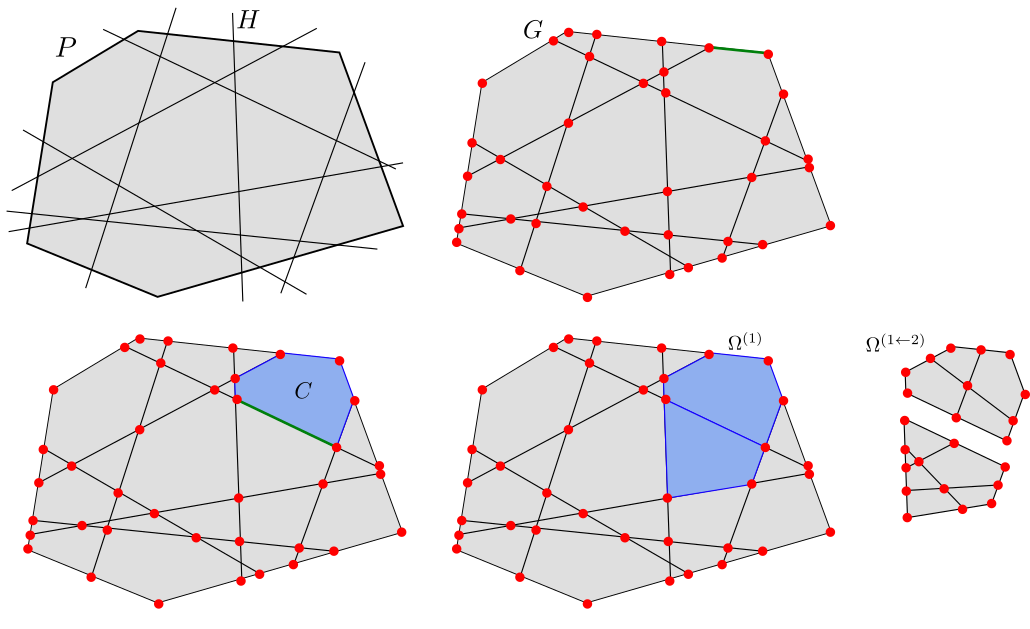
\includegraphics[width=0.8\linewidth]{drawings/splinecam_algorithm.png}
    \caption{The SplineCam visualisation procedure starts by identifying a two-dimensional region of interest $P$ and intersecting it with hyperplanes $H$, \textbf{upper left}. Then a graph $G$ is constructed using the points of intersection as nodes and the hyperplanes and region of interest as edges; an edge is then selected, \textbf{upper right}. A cycle from the selected edge is generated using a breadth first search to identify edges which are then connected in an order; one of the identified edges is then selected, \text{lower left}. With the selected edge, another cycled is formed as before to continue the formation of $\Omega^{(1)}$, \textbf{lower middle}. Once all cycles are identified, the regions are considered individually and intersected with the hyperplanes from the second layer, and the process repeats, \textbf{lower right}.}
    \label{fig:splinecam_algorithm}
\end{figure}

\begin{proposition}\label{prop:complexity_splinecam}
    Given a set of $n$ intersecting hyperplanes and a two-polytope $P$, Algorithm \ref{alg:cycles} has an average case complexity of $O\left(n^2\right)$.
\end{proposition}

\begin{tproof}
    The number of intersections and cycles induces by intersecting a polytope and hyperplanes is on the order less than or equal to $O\left(n^2\right)$. Therefore, the average case complexity of Algorithm \ref{alg:cycles} is also of the order $O\left(n^2\right)$.
\end{tproof}

\section{References}

Chapter \ref{ch:visualisation} from \cite{humayunSplineCamExactVisualization2023}.

\chapter{Complexity Measures}

\section{Introduction}

Deep networks can become highly over-parameterized, in the classical sense, and thus can approximate even randomly generated training data. Despite this capacity, they are typically arrive at solutions that generalise to unseen data in a way that cannot be accounted for by memorising the training. The development of complexity measures aims at investigating this phenomena in computationally tractable ways; with the intention on illuminating deep network training beyond loss curves, or providing tools the regularise the training process. In this chapter we explore how the tools of Part \ref{part:theoretical_foundations} can be utilised to construct complexity measures for deep networks.

\section{Local Complexity}\label{sec:local_complexity}

Let $V=\left(\mathbf{v}_1,\dots,\mathbf{v}_p\right)^\top$ be a matrix of vertices in a deep network's input space. Let $\mathcal{V}=\mathrm{conv}(V)$. Recall that the partition of the input space of layer $\ell$ can be expressed as the set of hyperplanes $$\partial\Omega=\bigcup_{i=1}^{d^{(\ell)}}\mathcal{H}^{(\ell)}_i,$$where $$\mathcal{H}^{(\ell)}_i=\left\{\mathbf{z}\in\mathbb{R}^{d^{(\ell-1)}}:\left\langle\left[W^{(\ell)}\right]_i,\mathbf{z}\right\rangle+\left[b^{(\ell)}\right]_i=0\right\}.$$One gauge the local complexity of $\mathcal{V}$ induced by layer $\ell$ by counting the number of regions in $$\mathcal{V}^{(\ell)}\cap\partial\Omega=\bigcup_{i=1}^{d^{(\ell)}}\mathcal{V}^{(\ell)}\cap\mathcal{H}^{(\ell)}_i,$$where $\mathcal{V}^{(\ell)}$ is the embedded representation of $\mathcal{V}$ after layer $\ell-1$ of the deep network. In particular, this will be on the order of $\mathcal{N}^{d^{(\ell-1)}}$, where $$\mathcal{N}=\left\vert\left\{i:i=1,\dots,d^{(\ell)}\text{ and }\mathcal{H}^{(\ell)}_i\cap\mathcal{V}^{(\ell)}\neq\emptyset\right\}\right\vert,$$which can thus be used as a proxy for the local complexity of $\mathcal{V}^{(\ell-1)}$. For practical tractability it is convenient to work with the convex hull of $V^{(\ell)}$\footnote{The matrix $\left(\mathbf{v}^{(1)},\dots,\mathbf{v}^{(p)}\right)^\top$, where $\mathbf{v}^{(\ell)}_i$ is the embedded representation of $\mathbf{v}_i$ after layer $\ell-1$ of the deep network.} which we will denote $\hat{\mathcal{V}}^{(\ell)}$.

\section{Absolute Deviation}\label{sec:absolute_deviation}

\subsection{Adaptive Linear Region Discovery}

For a hyperplane $\mathcal{H}^{(\ell)}_i\subseteq\mathbb{R}^{d^{(\ell-1)}}$, suppose that $\mathbf{z}^{(\ell-1)}(\mathbf{x})$ lies on its negative side.\footnote{If $\mathbf{z}^{(\ell-1)}(\mathbf{x})$ is on the positive side, flip the inequality and sign of $\lambda^{(\ell)}_j$ in \eqref{eq:adaptive_linear_region_min_problem}.}Then the smallest displacement $\lambda^{(\ell)}_j$ along a direction $\mathbf{d}\in\mathbb{R}^{d}$, that is non-zero and not lying in $\mathcal{H}^{(\ell)}_j$, required to cross $\mathcal{H}^{(\ell)}_j$ is
\begin{align}\label{eq:adaptive_linear_region_min_problem}
    \lambda^{(\ell)}_j&=\min_{\lambda\in\mathbb{R}}\left(\left[W^{(\ell)}\right]_{j,\cdot}^\top\left(\mathbf{z}^{(\ell-1)}+\lambda\mathbf{d}^{(\ell)}\right)+\left[b^{(\ell)}\right]_j>0\right)\nonumber\\&=\min_{\lambda\in\mathbb{R}}\left(\lambda>\frac{-\left[W^{(\ell)}\right]_{j,\cdot}^\top\mathbf{z}^{(\ell-1)}-\left[b^{(\ell)}\right]_j}{\left[W^{(\ell)}\right]_{j,\cdot}^\top\mathbf{d}^{(\ell)}}\right),
\end{align}
where $\mathbf{d}^{(\ell)}\in\mathbb{R}^{d^{(\ell-1)}}$ is the direction $\mathbf{d}$ in the input space of layer $\ell$, namely $\mathbf{d}^{(\ell)}=A_{\omega_{\mathbf{s}^{(1\leftarrow\ell)}\left(\mathbf{x}\right)}}^{(1\leftarrow\ell)}\mathbf{d}$.

In practice, the condition $\vert\lambda\vert>\tau$ for a sensitivity parameter $0<\tau\ll1$ is added to \eqref{eq:adaptive_linear_region_min_problem}, to ensure that a sufficient step is taken along $\mathbf{d}$ to traverse the boundary.

\begin{algorithm}
\caption{Minimum displacement finder.}\label{alg:min_displacement_finder}
\begin{algorithmic}
\Require $\mathbf{x}$, $\mathbf{d}$
\For{$\ell=1,\dots,L$}
\State $\lambda\leftarrow\infty$.
\State $\text{lambdas}\leftarrow\emptyset$.
\State $\text{lambdas}\leftarrow\frac{-b^{(\ell)}-W^{(\ell)}\mathbf{x}}{W^{(\ell)}\mathbf{d}}$. \Comment{Division is element-wise.}
\If{$\min(\text{lambdas})<\lambda$}
\State $\lambda\leftarrow\min(\text{lambdas})$.
\EndIf
\State $\mathbf{x}\leftarrow A^{(\ell)}_{\omega_{\mathbf{s}^{(\ell)}\left(\mathbf{x}\right)}}\mathbf{x}+b^{(\ell)}_{\omega_{\mathbf{s}^{(\ell)}\left(\mathbf{x}\right)}}$.
\State $\mathbf{d}\leftarrow A^{(\ell)}_{\omega_{\mathbf{s}^{(\ell)}\left(\mathbf{x}\right)}}\mathbf{d}$.
\EndFor
\State \Return $\text{lambdas}$.
\end{algorithmic}
\end{algorithm}

Given a $\mathbf{x}\in\mathbb{R}^d$ and a direction $\mathbf{d}$, the smallest displacement $\lambda$ in direction $\mathbf{d}$ to a region is given by iteratively solving \eqref{eq:adaptive_linear_region_min_problem} for each layer, namely $$\lambda=\min_{1\leq\ell\leq L,1\leq j\leq d^{(\ell-1)}}\lambda_j^{(\ell)},$$as summarised in Algorithm \ref{alg:min_displacement_finder}.

Iterating this procedure, it is possible to discover all regions along a path $\boldsymbol{\pi}:[0,1]\to\mathbb{R}^d$ given by $\boldsymbol{\pi}(t)=\mathbf{x}+t\mathbf{d}$. Since by the convexity of the regions, they induce a partition 
\begin{equation}\label{eq:path_region_partition}
    \mathcal{P}=\left\{t\in[0,1]:0=t_0<\dots<t_n=1\right\}.
\end{equation}
Letting $\mathcal{J}_i=\left[t_i,t_{i+1}\right]$, it follows that with $\tau<\min_{i=1,\dots,n}\left\vert\mathcal{J}_i\right\vert$ Algorithm \ref{alg:alrd_one_d} recovers all the regions, otherwise it recovers the regions with size larger than $\tau$.

\begin{algorithm}
\caption{Adaptive linear region discovery on compact one-dimensional domains.}\label{alg:alrd_one_d}
\begin{algorithmic}
\Require $\mathbf{x}_0$, $\mathbf{x}_1$, $\tau$
\State $\mathbf{c}\leftarrow\mathbf{s}\left(f\left(\mathbf{x}_0\right)\right)$.\Comment{Computed element-wise.}
\State $\mathbf{c}_1\leftarrow\mathbf{s}\left(f\left(\mathbf{x}_1\right)\right)$.
\State $\mathbf{d}\leftarrow\frac{\mathbf{x}_1-\mathbf{x}_0}{\left\Vert\mathbf{x}_1-\mathbf{x}_0\right\Vert_2}$.
\State $\mathcal{P}\leftarrow\emptyset$.
\While{$\mathbf{c}\neq\mathbf{c}_1$}
\State $\lambda\leftarrow$ Algorithm \ref{alg:min_displacement_finder}$(\mathbf{x},\mathbf{d})$.
\State $\mathcal{P}\leftarrow\mathcal{P}\cup\{\lambda\}$.
\If{$\lambda=\infty$}
\State \textbf{break}
\EndIf
\State $\mathbf{x}\leftarrow\mathbf{x}+\lambda\mathbf{d}$.
\If{$\left\Vert\mathbf{x}_0-\mathbf{x}_1\right\Vert_2<\left\Vert\mathbf{x}-\mathbf{x}_0\right\Vert_2$}
\State \textbf{break}
\EndIf
\State $\mathbf{c}\leftarrow\mathbf{s}(f(\mathbf{x}))$.
\EndWhile
\State \Return $\mathcal{P}$.
\end{algorithmic}
\end{algorithm}

\subsection{Quantifying Nonlinearity}

For distinct points $\mathbf{x}_0,\mathbf{x}_1\in\mathbb{R}^d$ let $g$ be an interpolation of $f_{\omega_{\mathbf{s}\left(\mathbf{x}_0\right)}}$ and $f_{\omega_{\mathbf{s}\left(\mathbf{x}_1\right)}}$ such that $$g\left(\mathbf{x}_0+t\left(\mathbf{x}_1-\mathbf{x}_0\right)\right)=f\left(\mathbf{x}_0\right)+t\left(f\left(\mathbf{x}_1\right)-f\left(\mathbf{x}_0\right)\right).$$

\begin{definition}
    The absolute deviation between distinct points $\mathbf{x}_0,\mathbf{x}_1\in\mathbb{R}^d$ is $$\mathbf{a}\left(\mathbf{x}_0,\mathbf{x}_1\right)=\int_{\pi}\left\vert f(\mathbf{x})-g(\mathbf{x})\right\vert\,\mathrm{d}\mathbf{x},$$where $\boldsymbol{\pi}:[0,1]\to\mathbb{R}^d$ is given by $\boldsymbol{\pi}(t)=\mathbf{x}_0+t\left(\mathbf{x}_1-\mathbf{x}_0\right)$.\footnote{In practice, often the $\ell_2$ norm of $\mathbf{a}\left(\mathbf{x}_0,\mathbf{x}_1\right)$ is considered instead as a scalar score.} 
\end{definition}

\begin{figure}
    \centering
    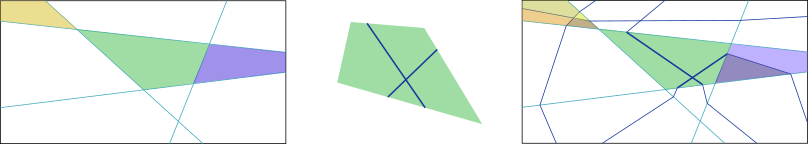
\includegraphics[width=0.75\linewidth]{drawings/iterative_partitioning_procedure.png}
    \caption{An illustration of what our notation for absolute deviation means in the context deep networks with a one-dimensional input domain. The region shaded in green represents the absolute deviation.}
    \label{fig:absolute_deviation}
\end{figure}

\begin{proposition}
    Recall that a deep network's regions induces a partition on $[0,1]$ \eqref{eq:path_region_partition}. For $j=1,\dots,d^{(L)}$ we have
    \begin{align*}
        \int_{\boldsymbol{\pi}}\left\vert\left[f(\mathbf{x})\right]_j-\left[\mathbf{a}(\mathbf{x})\right]_j\right\vert\,\mathrm{d}\mathbf{x}=\Vert\mathbf{d}\Vert\Bigg(\sum_{i=0}^{n-1}&\left(t_{\star}-t_i\right)\left\vert\left[f_{\omega_i}\left(\mathbf{x}_0\right)\right]_j-\left[f_{\omega_0}\left(\mathbf{x}_0\right)\right]_j\right\vert\\+&\left(t_{i+1}-t_{\star}\right)\left\vert\left[f_{\omega_i}\left(\mathbf{x}_0\right)\right]_j-\left[f_{\omega_0}\left(\mathbf{x}_0\right)\right]_j\right\vert\\+&\frac{t_{\star}^2-t_i^2}{2}\left\vert\left[f_{\omega_i}\left(\mathbf{x}_1\right)\right]_j-\left[f_{\omega_i}\left(\mathbf{x}_0\right)\right]_j-\left[f_{\omega_1}\left(\mathbf{x}_1\right)\right]_j+\left[f_{\omega_0}\left(\mathbf{x}_0\right)\right]_j\right\vert\\+&\frac{t_{i+1}^2-t_{\star}^2}{2}\left\vert\left[f_{\omega_i}\left(\mathbf{x}_1\right)\right]_j-\left[f_{\omega_i}\left(\mathbf{x}_0\right)\right]_j-\left[f_{\omega_1}\left(\mathbf{x}_1\right)\right]_j+\left[f_{\omega_0}\left(\mathbf{x}_0\right)\right]_j\right\vert\Bigg),
    \end{align*}
    where $t_{\star}=\max\left(t_i,\min\left(z_i,t_{i+1}\right)\right)$ for $$z_i=\frac{\left[f_{\omega_0}\left(\mathbf{x}_0\right)\right]_j-\left[f_{\omega_i}\left(\mathbf{x}_0\right)\right]_j}{\left[f_{\omega_i}\left(\mathbf{x}_1\right)\right]_j-\left[f_{\omega_i}\left(\mathbf{x}_0\right)\right]_j-\left[f_{\omega_1}\left(\mathbf{x}_1\right)\right]_j-\left[f_{\omega_0}\left(\mathbf{x}_0\right)\right]_j},$$and where $f_{\omega_i}$ denotes the affine function of the deep network operating on the region corresponding to $t_i$ in $\mathcal{P}$.
\end{proposition}

\begin{tproof}
    Initially, we obtain that
    \begin{align*}
        \int_{\boldsymbol{\pi}}&\left\vert\left[f(\mathbf{x})\right]_j-\left[\mathbf{a}(\mathbf{x})\right]_j\right\vert\,\mathrm{d}\mathbf{x}\\&=\sum_{i=0}^{n-1}\int_{t_i}^{t_{i+1}}\left\vert\left[f(\boldsymbol{\pi}(t))\right]_j-\left[\mathbf{a}(\boldsymbol{\pi}(t))\right]_j\right\vert\left\Vert\dot{\boldsymbol{\pi}}(t)\right\Vert\,\mathrm{d}t\\&=\sum_{i=0}^{n-1}\int_{t_i}^{t_{i+1}}\left\vert\left[f\left(\mathbf{x}_0+t\mathbf{d}\right)\right]_j-\left[\mathbf{a}\left(\mathbf{x}_0+t\mathbf{d}\right)\right]_j\right\vert\Vert\mathbf{d}\Vert\,\mathrm{d}t\\&=\Vert\mathbf{d}\Vert\sum_{i=0}^{n-1}\int_{t_i}^{t_{i+1}}\left\vert\left[f_{\omega_i}\left(\mathbf{x}_0\right)\right]_j-\left[f_{\omega_0}\left(\mathbf{x}_0\right)\right]_j+t\left(\left[f_{\omega_i}\left(\mathbf{x}_1\right)\right]_j-\left[f_{\omega_i}\left(\mathbf{x}_0\right)\right]_j-\left[f_{\omega_1}\left(\mathbf{x}_1\right)\right]_j+\left[f_{\omega_0}\left(\mathbf{x}_0\right)\right]_j\right)\right\vert\,\mathrm{d}t.
    \end{align*}
    Now the integrand is not necessarily monotonic, in particular, on $\omega_i$ the functions $\left[f\right]_j$ and $\left[\mathbf{a}\right]$ may intersect at $$z_i=\frac{\left[f_{\omega_0}\left(\mathbf{x}_0\right)\right]_j-\left[f_{\omega_i}\left(\mathbf{x}_0\right)\right]_j}{\left[f_{\omega_i}\left(\mathbf{x}_1\right)\right]_j-\left[f_{\omega_i}\left(\mathbf{x}_0\right)\right]_j-\left[f_{\omega_1}\left(\mathbf{x}_1\right)\right]_j-\left[f_{\omega_0}\left(\mathbf{x}_0\right)\right]_j}.$$If $z_i\not\in\left(t_i,t_{i+1}\right)$, then we need not worry about this intersection for the computation of the integral, otherwise we can separate the integral across the domains $\left[t_i,z_i\right]$ and $\left[z_i,t_{i+1}\right]$. In any case, we can take $t_{\star}=\max\left(t_i,\min\left(z_i,t_{i+1}\right)\right)$ and consider the integral over the domains $\left[t_i,t_{\star}\right]$ and $\left[t_{\star},t_{i+1}\right]$ on which our integrand will be affine. Therefore,
    \begin{align*}
        \int_{\boldsymbol{\pi}}&\left\vert\left[f(\mathbf{x})\right]_j-\left[\mathbf{a}(\mathbf{x})\right]_j\right\vert\,\mathrm{d}\mathbf{x}\\&=\Vert\mathbf{d}\Vert\sum_{i=0}^{n-1}\int_{t_i}^{t_{\star}}\left\vert\left[f_{\omega_i}\left(\mathbf{x}_0\right)\right]_j-\left[f_{\omega_0}\left(\mathbf{x}_0\right)\right]_j+t\left(\left[f_{\omega_i}\left(\mathbf{x}_1\right)\right]_j-\left[f_{\omega_i}\left(\mathbf{x}_0\right)\right]_j-\left[f_{\omega_1}\left(\mathbf{x}_1\right)\right]_j+\left[f_{\omega_0}\left(\mathbf{x}_0\right)\right]_j\right)\right\vert\,\mathrm{d}t\\&+\Vert\mathbf{d}\Vert\sum_{i=0}^{n-1}\int_{t_{\star}}^{t_{i+1}}\left\vert\left[f_{\omega_i}\left(\mathbf{x}_0\right)\right]_j-\left[f_{\omega_0}\left(\mathbf{x}_0\right)\right]_j+t\left(\left[f_{\omega_i}\left(\mathbf{x}_1\right)\right]_j-\left[f_{\omega_i}\left(\mathbf{x}_0\right)\right]_j-\left[f_{\omega_1}\left(\mathbf{x}_1\right)\right]_j+\left[f_{\omega_0}\left(\mathbf{x}_0\right)\right]_j\right)\right\vert\,\mathrm{d}t,
    \end{align*}
    which simplifies to the desired expression.
\end{tproof}

\section{Hessian Based Rugosity Measure}\label{sec:hessian_rugosity}

Throughout this section we'll be consider a deep network $f:\mathbb{R}^d\to\mathbb{R}$ and a set of training data $\left\{\left(\mathbf{x}_i,y_i\right)\right\}_{i=1}^n$ where $\mathbf{x}_i\in\mathbb{R}^d$ and $y_i\in\mathbb{R}$ for $i=1,\dots,n$. In particular, we assume that the points $\left\{\mathbf{x}_i\right\}_{i=1}^n$ lie close to an $m$-dimensional manifold $\mathcal{M}\subseteq\mathbb{R}^d$.

\subsection{Smooth Activation Deep Networks}

Suppose that $f$ employs smooth activation operators. For $p\geq1$ let $$C_p(f):=\left(\int_{\mathcal{M}}\left\Vert\nabla^2_{\text{tan}}f(\mathbf{x})\right\Vert^p_F\,\mathrm{d}\mathbf{x}\right)^{\frac{1}{p}},$$where $\nabla^2_{\text{tan}}f(\mathbf{x})$ is the Hessian of $f$ at $\mathbf{x}$ in the coordinates of the $m$-dimensional affine space tangent to the manifold at $\mathbf{x}\in\mathcal{M}$.

The quantity $C_p(f)$ measure the average \emph{curviness} of $f$ over $\mathcal{M}$. More specifically, it is zero if and only if $f$ is an affine function on $\mathcal{M}$.

As $f$ is smooth, we have $$\nabla^2f(\mathbf{x})\mathbf{u}=\lim_{\epsilon\to0}\left(\frac{\nabla f(\mathbf{x}+\epsilon\mathbf{u})-\nabla f(\mathbf{x})}{\epsilon}\right).$$Moreover, for $\mathbf{u}\in\mathbb{R}^d$ chosen uniformly at random on the unit sphere, we have $$\mathbb{E}\left(\left\Vert A\mathbf{u}\right\Vert_2^2\right)=\mathbb{E}\left(\sum_{i,j=1,\dots,d}[\mathbf{u}]_i[\mathbf{u}]_j\left[A^\top A\right]_{ij}\right)=\frac{\Vert A\Vert_F^2}{d},$$for any $A\in\mathbb{R}^{d\times d}$. Therefore, we can obtain a Monte Carlo approximation for $C_p(f)$ on the training data as $$\tilde{C}_{p,\epsilon}(f)=\left(\frac{d^{\frac{p}{2}}}{n\epsilon^p\hat{n}^{\frac{p}{2}}}\sum_{i=1}^n\left(\sum_{j=1}^{\hat{n}}\left\Vert\nabla f\left(\mathbf{x}_i+\epsilon\mathbf{u}_j\right)-\nabla f\left(\mathbf{x}_i\right)\right\Vert_2^2\right)\right)^{\frac{1}{p}},$$where $\epsilon>0$ is small and the $\mathbf{u}_j$ are uniform samples of unit vectors on the $m$-dimensional subspace tangent to $\mathcal{M}$ at $\mathbf{x}$. This just follows from the observation that $$$$

\subsection{Continuous Piecewise Affine Deep Networks}

For $f$ employing piecewise affine activation operators, it can be characterised as a continuous piecewise affine operator. In particular, recall the notation convention from statement 2 of Remark \ref{rem:affine_spline}, we have that $f(\mathbf{x})=A[\mathbf{x}]\mathbf{x}+b[\mathbf{x}]$, where $A[\mathbf{x}]$ and $b[\mathbf{x}]$ are the parameters for the affine function on the region encompassing $\mathbf{x}$.

The Hessian for $f$ is not well-defined, however, we can extend a definition of the Hessian to encompass this case. Let $\epsilon>0$. Then for $\mathbf{x}\in\mathbb{R}^d$ not on the boundary of a partition and a unit vector $\mathbf{u}$, let $$H^{\epsilon}_{\mathbf{u}}(\mathbf{x})=\begin{cases}\frac{A\left[\mathbf{x}+\epsilon\mathbf{u}\right]-A[\mathbf{x}]}{\epsilon}&\mathbf{u}\text{ in tangent manifold of }\mathcal{M}\text{ at }\mathbf{x}\\\mathbf{0}&\text{otherwise}.\end{cases}$$With this, for $p\geq1$, let $$C_{p,\epsilon}:=\sqrt{d}\left(\int_{\mathcal{M}}\left(\mathbb{E}_{\mathbf{u}}\left(\left\Vert H_{\mathbf{u}}^{\epsilon}(\mathbf{x})\right\Vert_2^2\right)\right)^{\frac{p}{2}}\right)^{\frac{1}{p}},$$where $\mathbf{u}$ is uniform over the unit sphere.

A Monte Carlo approximation for $C_{p,\epsilon}(f)$ on the training data can be obtained as 
\begin{equation}\label{eq:monte_carlo_rugosity_cpa}
    \tilde{C}_{p,\epsilon}(f)=\left(\frac{d^{\frac{p}{2}}}{n\epsilon^p\hat{n}^{\frac{p}{2}}}\sum_{i=1}^n\left(\sum_{j=1}^{\hat{n}}\left\Vert A\left[\mathbf{x}_i+\epsilon\mathbf{u}_j\right]-A\left[\mathbf{x}_i\right]\right\Vert_2^2\right)\right)^{\frac{1}{p}},
\end{equation}
where the $\mathbf{u}_j$ are uniform samples of unit vectors on the $m$-dimensional subspace tangent to $\mathcal{M}$ at $\mathbf{x}$.

\subsection{Connection to Data Augmentation}

The process of data augmentation takes the original dataset $\left\{\left(\mathbf{x}_i,y_i\right)\right\}_{i=1}^n$ and generates the augmented dataset $\left\{\left\{\left(\mathbf{x}_i+\mathbf{u}_{ij},y_i\right)\right\}_{j=0}^{\hat{n}}\right\}_{i=1}^n$ by applying transformations to the points $\mathbf{x}_i$ such that they continue to lie on $\mathcal{M}$. In this case, we are using $\mathbf{u}_{i0}$ to represent the identity transformation on $\mathbf{x}_i$. Training $f$ on the original dataset involves minimizing a loss $$\mathcal{L}:=\sum_{i=1}^\ell\left(f\left(\mathbf{x}_i\right),y_i\right),$$where we are assuming $\ell$ is convex. On the augmented dataset the corresponding loss is $$\mathcal{L}_{\text{aug}}:=\frac{1}{\hat{n}+1}\sum_{i=1}^n\left(\ell\left(f\left(\mathbf{x}_i\right),y_i\right)+\sum_{j=1}^{\hat{n}}\ell\left(f\left(\mathbf{x}_i+\mathbf{u}_{ij}\right),y_i\right)\right).$$

\begin{theorem}
    Let $f$ be a deep network that is a continuous piecewise affine operator. Assume that $\left\Vert\mathbf{x}_i\right\Vert_2\leq R$, that $f$ has Lipschitz constant $K_1$, and that $\ell$ has Lipschitz constant $K_2$. Then for $\left\Vert\mathbf{u}_{ij}\right\Vert_2\leq\epsilon$ we have 
    \begin{align}
        \mathcal{L}_{\text{aug}}\leq\mathcal{L}&+\frac{RK_2}{\hat{n}+1}\underbrace{\sum_{i=1}^n\sum_{j=1}^{\hat{n}}\left\Vert A\left[\mathbf{x}_i+u_{ij}\right]-A\left[\mathbf{x}_i\right]\right\Vert_2}_{\hat{C}(f)}\nonumber\\&+\frac{K_2}{\hat{n}+1}\sum_{i=1}^n\sum_{j=1}^{\hat{n}}\left\vert b\left[\mathbf{x}_i+\mathbf{u}_{ij}\right]-b\left[\mathbf{x}_i\right]\right\vert\nonumber\\&+\frac{K_1K_2\hat{n}n\epsilon}{\hat{n}+1}+o(\epsilon).
    \end{align}
\end{theorem}

\begin{tproof}
    Observe that
    \begin{align*}
        \ell\left(f\left(\mathbf{x}_i+\mathbf{u}_{ij}\right),y_i\right)&=\ell\left(A\left[\mathbf{x}_i+\mathbf{u}_{ij}\right]\left(\mathbf{x}_i+\mathbf{u}_{ij}\right)+b\left[\mathbf{x}_i+\mathbf{u}_{ij}\right],y_i\right)\\&=\ell\big(A\left[\mathbf{x}_i\right]\mathbf{x}_i+b\left[\mathbf{x}_i\right]+\left(A\left[\mathbf{x}_i+\mathbf{u}_{ij}\right]-A\left[\mathbf{x}_i\right]\right)\mathbf{x}_i\\&\qquad+\left(b\left[\mathbf{x}_i+\mathbf{u}_{ij}\right]-b\left[\mathbf{x}_i\right]\right)+A\left[\mathbf{x}_i+\mathbf{u}_{ij}\right]\mathbf{u}_{ij},y_i\big).
    \end{align*}
    Therefore, the first-order approximation of $\ell\left(f\left(\mathbf{x}_i+\mathbf{u}_{ij}\right),y_i\right)$ around $\ell\left(f\left(\mathbf{x}_ir\right),y_i\right)$ is 
    \begin{align*}
        \tilde{\ell}\left(f\left(\mathbf{x}_i+\mathbf{u}_{ij}\right),y_i\right)=&\ell\left(f\left(\mathbf{x}_ir\right),y_i\right)\\&+\big(\left(A\left[\mathbf{x}_i+\mathbf{u}_{ij}\right]-A\left[\mathbf{x}_i\right]\right)\mathbf{x}_i\\&\qquad+\left(b\left[\mathbf{x}_i+\mathbf{u}_{ij}\right]-b\left[\mathbf{x}_i\right]\right)+A\left[\mathbf{x}_i+\mathbf{u}_{ij}\right]\mathbf{u}_{ij}\big)^\top\nabla_{f\left(\mathbf{x}_i\right)}\ell\left(f\left(\mathbf{x}_i\right),y_i\right).
    \end{align*}
    Hence, 
    \begin{align*}
        \tilde{\ell}\left(f\left(\mathbf{x}_i+\mathbf{u}_{ij}\right),y_i\right)\leq&\ell\left(f\left(\mathbf{x}_ir\right),y_i\right)+RK_2\left\Vert A\left[\mathbf{x}_i+\mathbf{u}_{ij}\right]-A\left[\mathbf{x}_i\right]\right\Vert_2\\&+K_2\left\vert b\left[\mathbf{x}_i+\mathbf{u}_{ij}\right]-b\left[\mathbf{x}_i\right]\right\vert+\epsilon K_1K_2.
    \end{align*}
    Therefore, 
    \begin{align*}
        \tilde{\mathcal{L}}_{\text{aug}}&=\frac{1}{\hat{n}+1}\sum_{i=1}^n\left(\ell\left(f\left(\mathbf{x}_ir\right),y_i\right)+\sum_{j=1}^{\hat{n}}\tilde{\ell}\left(f\left(\mathbf{x}_i+\mathbf{u}_{ij}\right),y_i\right)\right)\\&\leq\mathcal{L}+\frac{RK_2}{\hat{n}+1}\sum_{i=1}^n\sum_{j=1}^{\hat{n}}\left\Vert A\left[\mathbf{x}_i+\mathbf{u}_{ij}\right]-A\left[\mathbf{x}_i\right]\right\Vert_2\\&\quad+\frac{K_2}{\hat{n}+1}\sum_{i=1}^n\sum_{j=1}^{\hat{n}}\left\vert b\left[\mathbf{x}_i+\mathbf{u}_{ij}\right]-b\left[\mathbf{x}_i\right]\right\vert+\frac{K_1K_2n\hat{n}\epsilon}{\hat{n}+1},
    \end{align*}
    completing the proof.
\end{tproof}

\begin{remark}
    Note how for $p=1$, \eqref{eq:monte_carlo_rugosity_cpa} is very similar to $\hat{C}(f)$, up to a normalisation constant. Moreover, the data augmentations methods are such that $\mathbf{x}_i+\mathbf{u}_{ij}\in\mathcal{M}$. Thus, a sufficiently rich set of small augmentations will have similar distribution and support to the uniform distribution over unit vectors on the subspace tangent to the manifold, as is the case in \eqref{eq:monte_carlo_rugosity_cpa}. Therefore, the Hessian-based rugosity measure \eqref{eq:monte_carlo_rugosity_cpa} could act as an explicit regularisation term in training that yields similar benefits as data augmentation, namely minimising $\mathcal{L}_{\text{aug}}$.
\end{remark}

\section{References}

Section \ref{sec:local_complexity} from \citet{humayunDeepNetworksAlways2024}. Section \ref{sec:absolute_deviation} from \citet{gambaAreAllLinear2022}. Section \ref{sec:hessian_rugosity} from \citet{lejeuneImplicitRugosityRegularization2019}.

\chapter{Constraining Optimization}\label{ch:constraining_optimization}

\section{Introduction}

By understanding the functional geometry of deep networks and how this relates to their properties we can impose certain properties on deep networks by intervening on this geometry. More specifically, by imposing constraints in the optimization process, one can provide guarantees on the behaviour of a trained network by guaranteeing its functional geometry. Here we explore how this is done in practice and its application to ensuring the robustness of deep networks around training points.

\section{POLICE}\label{sec:police}

Deep networks struggle on optimization problems involving exact constraints, such as $$\begin{cases}\min_{\theta}\left\Vert f_{\theta}-f^*\right\Vert+\lambda\mathcal{R}(\theta)\\f_{\theta}(\mathbf{x})\text{ affine on }R.\end{cases}$$

Let $V=\left(\mathbf{v}_1,\dots,\mathbf{v}_p\right)^\top$ be a matrix of $p$ vertices, such that 
\begin{equation}\label{eq:region_approx_convex_hull}
    R\approx\left\{V^\top\alpha:\alpha_j\geq0\,\text{ for all }j\,\text{ and }\alpha^\top\mathbf{1}=1\right\}.
\end{equation}
Let $\mathbf{v}_j^{(\ell)}$ be the mapping of the $j^{\text{th}}$ vertex through layers $1$ through $\ell-1$, similarly for $V^{(\ell)}$ and with $\mathbf{v}_j$ corresponding to $\ell=1$.

Henceforth, for simplicity, we will assume that \eqref{eq:region_approx_convex_hull} holds exactly.

\begin{theorem}\label{thm:nec_suf_to_stay_affine}
    A necessary and sufficient condition for a continuous-piecewise affine spline deep network to stay affine within a region $R$, is to have the same pre-activation sign patterns between the vertices $\mathbf{v}_j$ for every $j=1,\dots,p$ and each layer.
\end{theorem}

\begin{proof}
    If $\mathrm{sign}\left(f^{(1)}(\mathbf{v}_i)\right)=\mathrm{sign}\left(f^{(1)}(\mathbf{v}_j)\right)$ for all $i,j\in\{1,\dots,p\}$, then the vertices all lie within the same partition region of $\Omega^{(1)}$. That is, there exists $\omega^*\in\Omega^{(1)}$ such that $v_j\in\omega^*$ for all $j\in\{1,\dots,P\}$. Since, $\omega^*$ is convex due to  Corollary \ref{cor:deep_network_layer_convex_polytopes}, and $R$ is convex by construction, it follows that $R\subseteq\omega^*$. Repeating this for each layer, we arrive at the conclusion that the input-output mapping of the deep network as affine within $R$.
\end{proof}

\begin{proposition}
    A sufficient condition for layer $\ell$ to be linear within the input space region given by $R$ is
    \begin{equation}\label{eq:condition_to_ensure_nec_suf}
        0\leq\min_{(i,j)\in[p]\times\left[d^{(\ell)}\right]}H_{i,j}s_j,
    \end{equation}
    where $H=V^{(\ell)}\left(W^{(\ell)}\right)^\top+\mathbf{1}\left(b^{(\ell)}\right)^\top$ and $$s_j=\begin{cases}\left\vert\left\{i:H_{i,j}>0\right\}\right\vert\geq\frac{p}{2}\\-1&\text{otherwise.}\end{cases}$$
\end{proposition}

\begin{tproof}
    The matrix $H\in\mathbb{R}^{[p]\times d^{(\ell)}}$ is simply the pre-activation of layer $\ell$ given input $V^{(\ell)}$. Therefore, by Theorem \ref{thm:nec_suf_to_stay_affine}, it is sufficient to ensure that the rows of $H$ have the same sign pattern. Clearly enforcing \eqref{eq:condition_to_ensure_nec_suf} ensures this, with the construction of $s_j$ meaning that we are enforcing the sign based on majority.
\end{tproof}

Algorithm \ref{alg:police_train_time}, known as POLICE, implements condition \eqref{eq:condition_to_ensure_nec_suf} at train time to satisfy the condition of Theorem \ref{thm:nec_suf_to_stay_affine} which ensures the affinity of the input-output mapping on $R$. One can similarly implement the condition at test time using Algorithm \ref{alg:police_test_time}.

\begin{algorithm}
\caption{Provably Optimal Linear Constraint Enforcement. Train time.}\label{alg:police_train_time}
\begin{algorithmic}
\Require $X\in\mathbb{R}^{n\times d}$, $V\in\mathbb{R}^{m\times d}$
\State $V^{(1)}\leftarrow V$.
\State $X\leftarrow X$.
\For{$\ell=1,\dots,L$}
\State $H\leftarrow V^{(\ell)}\left(W^{(\ell)}\right)^\top+\mathbf{1}\left(b^{(\ell)}\right)^\top$.
\State $s=\text{MajorityVote}\left(\mathrm{sign}(H),\text{axis}=0\right)$
\State $c=\mathrm{ReLU}\left(-H\mathrm{diag}(s)\right).\max(\text{axis}=0)\odot s$.
\State $X^{(\ell+1)}\leftarrow\sigma\left(X^{(\ell)}\left(W^{(\ell)}\right)^\top+\mathbf{1}\left(b^{(\ell)}+c\right)^\top\right)$.
\State $V^{(\ell+1)}\leftarrow\sigma\left(V^{(\ell)}\left(W^{(\ell)}\right)^\top+\mathbf{1}\left(b^{(\ell)}+c\right)^\top\right)$.
\EndFor
\end{algorithmic}
\end{algorithm}

\begin{algorithm}
\caption{Provably Optimal Linear Constraint Enforcement. Test time.}\label{alg:police_test_time}
\begin{algorithmic}
\Require $V\in\mathbb{R}^{m\times d}$
\State $V^{(1)}\leftarrow V$.
\For{$\ell=1,\dots,L$}
\State $H\leftarrow V^{(\ell)}\left(W^{(\ell)}\right)^\top+\mathbf{1}\left(b^{(\ell)}\right)^\top$.
\State $s=\text{MajorityVote}\left(\mathrm{sign}(H),\text{axis}=0\right)$
\State $c=\mathrm{ReLU}\left(-H\mathrm{diag}(s)\right).\max(\text{axis}=0)\odot s$.
\State $V^{(\ell+1)}\leftarrow\sigma\left(V^{(\ell)}\left(W^{(\ell)}\right)^\top+\mathbf{1}\left(b^{(\ell)}+c\right)^\top\right)$.
\State $b^{(\ell)}\leftarrow b^{(\ell)}+c$.
\EndFor
\end{algorithmic}
\end{algorithm}

\section{Instance Robustness}\label{sec:instance_robustness}

\begin{definition}\label{def:robust}
    A binary classifier deep network $f$ is $\epsilon$-robust at $\mathbf{x}\in\mathbb{R}^d$ if $$\left\{\mathbf{x}^\prime\in B_{\epsilon}(\mathbf{x}):f\left(\mathbf{x}^\prime\right)\neq f(\mathbf{x})\right\}=\emptyset.$$
\end{definition}

\begin{remark}
    \begin{enumerate}
        \item[]
        \item Definition \ref{def:robust} is formally saying that the minimum distance of $\mathbf{x}$ from the decision boundary of $f$ is lower bounded in $\ell_2$ norm by $\epsilon$.
        \item Recall that $$B_{\epsilon}(\mathbf{x})=\left\{\mathbf{x}^\prime:\left\Vert\mathbf{x}^\prime-\mathbf{x}\right\Vert\leq\epsilon\right\}.$$Note that the norm $\Vert\cdot\Vert$ in this instance is unspecified.
    \end{enumerate} 
\end{remark}

\begin{theorem}\label{thm:provable_instance_constraint}
    Consider a binary classifier $f$. For $\mathbf{x}\in\mathbb{R}^d$, if there exists a $d$-polytope containing $\mathbf{x}$ with $p\geq d$ vertices $V=\{\mathbf{v}_j\}_{j=1}^p$ of which $d$ form a basis, such that $\left\Vert\mathbf{v}_j-\mathbf{x}\right\Vert_1>\epsilon$ for each $\mathbf{v}_j\in V$ and 
    \begin{equation}\label{eq:condition_crop}
        \left\vert\sum_{j=1}^p\mathrm{sign}\left(\left\langle\left[W^{(L)}\right]_{1,\cdot},f^{(\ell-1)}(\mathbf{v}_j)\right\rangle+\left[b^{(L)}\right]_1\right)\right\vert=p,
    \end{equation}
    then $f$ is $\epsilon$-robust in $\ell_1$ norm at $\mathbf{x}$.
\end{theorem}

\begin{tproof}
    By construction $B_{\epsilon}(\mathbf{x})\subseteq\mathrm{conv}(V)$. Moreover, \eqref{eq:condition_crop} ensures that the pre-activation pattern between the vertices are the same, so by Theorem \ref{thm:nec_suf_to_stay_affine} we have that the output of the vertices, and in particular $\mathrm{conv}(V)$, are on the same side of the decision boundary. Meaning that the decision $B_{\epsilon}(\mathbf{x})$ remains on the same side of the decision boundary through the mapping, and hence the deep network is $\epsilon$ robust in $\ell_1$ norm.
\end{tproof}

From Theorem \ref{thm:provable_instance_constraint} its follows that one can use Algorithm \ref{alg:police_train_time} to train a deep network to be $\epsilon$-robust at a particular instance $\mathbf{x}\in\mathbb{R}^d$. By applying constraints to multiple samples and ensuring that the signs off all the constraints are the same, one can train a deep network to be $\epsilon$-robust at multiple samples.

\section{References}

Section \ref{sec:police} from \cite{balestrieroPoliceProvablyOptimal2023}. Section \ref{sec:instance_robustness} from \cite{humayunProvableInstanceSpecific2023}.

\chapter{Formal Verification}

\section{Introduction}

In Chapter \ref{ch:constraining_optimization} we looked at enforcing properties of deep networks by constraining the optimization process. In this chapter we focus on the similar problem of deriving guarantees on the properties of deep networks by analysing the optimized artefact. For example, just as we previously ensured the predictions of deep networks in convex hulls around training points in Section \ref{sec:instance_robustness}, in this chapter we will show how to guarantee predictions in regions of the input space. This broad field of guaranteeing deep network behaviour through mathematical arguments is known as formal verification.

\section{Predictions}

\begin{theorem}\label{thm:prediction_verification}
    Consider a binary classifier $f$ and let $\omega\in\Omega$ have vertices $\left\{\mathbf{v}_1,\dots,\mathbf{v}_p\right\}$. Then if $$\left\vert\sum_{j=1}^p\mathrm{sign}\left(\left\langle\left[W^{(L)}\right]_{1,\cdot},f^{(\ell-1)}\left(\mathbf{v}_j\right)\right\rangle+\left[b^{(L)}\right]_1\right)\right\vert=p,$$then $f$ makes the same classification prediction for every $\mathbf{x}\in\omega$. 
\end{theorem}

\begin{tproof}
    \TODO
\end{tproof}

\begin{remark}
    \begin{enumerate}
        \item[]
        \item Note the similarity between Theorem \ref{thm:prediction_verification} and Theorem \ref{thm:provable_instance_constraint}.
        \item From Theorem \ref{thm:prediction_verification}, it follows that it suffices to understand the predictions of the deep network at the vertices of a given region to make inferences on the predictions it will make for all points within the region $\omega$.
    \end{enumerate}
\end{remark}

\TODO
\begin{figure}
    \centering
    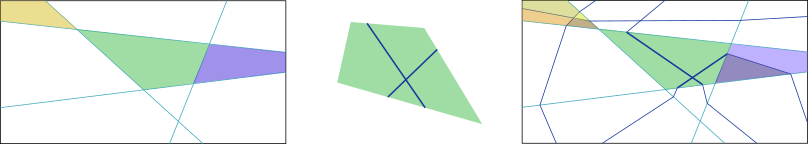
\includegraphics[width=0.8\linewidth]{drawings/iterative_partitioning_procedure.png}
    \caption{The training data is depicted as scatter points, colour-coded according to the class that they belong too. The highlighted regions correspond to regions for which it can be guaranteed that the deep network predicts the class associated to that colour.}
    \label{fig:prediction_verification}
\end{figure}

Typically, regions $\omega\in\Omega$ induced by $f:\mathbb{R}^d\to\mathbb{R}$ are bounded by on the order of $d$ vertices. Although it seems as though we can guarantee the behaviour of a deep network by only checking its behaviour on a relatively few number of determinable points, computing the points is computationally expensive. However, as shown in Section \ref{sec:splinecam}, this computations are tractable when we restrict ourselves to a two-dimensional slice of the input domain. If the input domain is two-dimensional, then we would be able to make statements such as the robustness of instances in our input domain.

\begin{example}
    Suppose that we have a deep network $f:\mathbb{R}^2\to\mathbb{R}$ comprising of four fully connected operators composed with ReLU non-linearities. We can train this deep network to perform two-class classification on a set of training data. Since $f$ is a continuous affine spline, it induces a partition of the input space. Let $P$ be a two-dimensional polytope encompassing the training data. Then using Algorithm \ref{alg:cycles} we can obtain the partition and thus the vertices bounding the regions of $\Omega$ intersecting $P$. We can then use Theorem \ref{thm:prediction_verification} to identify regions on which we can guarantee the predictions of our deep network, Figure \ref{fig:prediction_verification}. Of course, we can make $P$ arbitrarily larger to improve the strength of the inferred guarantees. However, this comes with additional computational costs as more regions $\omega$ would intersect $P$, resulting in the effects outlined in Proposition \ref{prop:complexity_splinecam}. For practical purposes, formal verification only really needs to be able to provide guarantees on likely inputs to our deep network. Clearly from observing the data in Figure \ref{fig:prediction_verification}, it is clear that $P$, and the verified region, captures a significant proportion of training data distribution.
\end{example}

In the case where our input domain has more than two-dimensions all is not lost, as certain properties of the input domain lie on two-dimensional subspaces; meaning we can verify predictions for specific properties in the input domain.

\begin{example}
    \begin{enumerate}
        \item[]
        \item Suppose that our deep network is receiving flattened images as its input. Then for an image $\mathbf{x}$, verifying predictions in the two-dimensional subspace spanned by $\mathbf{v}_1:=\frac{\mathbf{x}}{\Vert\mathbf{x}\Vert}$ and $\mathbf{v}_2=\text{gramschmidtvector}$ corresponds to verifying the predictions of the deep network as the brightness of the image $\mathbf{x}$ is varied.
        \item It has been shown that features of a deep network can correspond directions in input space of deep networks, Section \ref{sec:directions_as_units}. Therefore, verifying predictions in the two-dimensional spanned by these directions and an orthogonal direction corresponds to verifying the predictions of the deep network for inputs expressing this feature to various degrees.
    \end{enumerate}
\end{example}

\section{References}

\chapter{Pruning}\label{ch:pruning}

\section{Introduction}

In the classical statical sense deep networks are over-parametrised, and thus their optimisation should lead to degenerate solutions to the task at hand. However, it is observed in practice that deep networks arrive at remarkably generalisable solutions, despite having the capacity to memorise their training. This suggests that their in some redundancy in their capacity. Using our developed theory we can reason about how to judiciously reduce, or prune, parameters of the deep network in a manner that maintains its performance. Initially we formulate autoencoders to introduce the framework in which generative models operate in; then we focus on the generative component.

\section{Characterisation of Techniques}

Consider the $\ell^\text{th}$ layer of a deep network $$f^{(\ell)}(\mathbf{x})=\sigma\left(W^{(\ell)}+b^{(\ell)}\right),$$where $\sigma$ is a leaky ReLU with parameter $\eta$. Recall the induced a partition $\Omega^{(\ell)}$ of $\mathbb{R}^{d^{(\ell-1)}}$ given by  \eqref{eq:layer_partition_relu}, along with the functional decomposition of the layer operator \eqref{eq:functional_decomposition_layer_operator}.

A pruning strategy is equivalent to applying a mask onto the layer's parameters, $$\left(W^{(\ell)},b^{(\ell)}\right)\mapsto\left(M^{(\ell)}\odot W^{(\ell)},m^{(\ell)}\odot b^{(\ell)}\right),$$where $M^{(\ell)}\in\{0,1\}^{d^{(\ell)}\times d^{(\ell-1)}}$ and $m^{(\ell)}\in\{0,1\}^{d^{(\ell)}}$.

\begin{example}
    \begin{enumerate}
        \item[]
        \item Unit pruning would employ $M^{(\ell)}=\tilde{m}^{(\ell)}\mathbf{1}^\top$ and $m^{(\ell)}=\tilde{m}^{(\ell)}$.
        \item Parameter pruning would treat each entry of $M^{(\ell)}$ and $m^{(\ell)}$ independently.
    \end{enumerate}
\end{example}

\section{Impact on Partition}

\begin{proposition}
    Setting any entry of $M^{(\ell)}$ or $m^{(\ell)}$ to zero impacts the per-region affine mappings $A^{(\ell)}_{\omega}$ and $b^{(\ell)}_{\omega}$, as well as the input space partition $\Omega$.
\end{proposition}

\begin{tproof}
    This follows from the dependency of $A^{(\ell)}_{\omega}$, $b^{(\ell)}_{\omega}$ and $\Omega^{(\ell)}$ on $W^{(\ell)}$ and $b^{(\ell)}$ highlighted in \eqref{eq:layer_partition_relu} and \eqref{eq:functional_decomposition_layer_operator}.
\end{tproof}

Let $\left\vert\Omega^{(\ell)};W^{(\ell)},b^{(\ell)}\right\vert$ denote the number of regions in $\Omega^{(\ell)}$ when the layer is parametrized by $W^{(\ell)}$ and $b^{(\ell)}$.

\begin{theorem}
    We have $$\left\vert\Omega^{(\ell)};M^{(\ell)}\odot W^{(\ell)},m^{(\ell)}\odot b^{(\ell)}\right\vert\leq\left\vert\Omega^{(\ell)};W^{(\ell)},b^{(\ell)}\right\vert-\sum_{k=1}^{d^{(\ell)}}\mathbf{1}\left(\left\langle\left[M^{(\ell)}\right]_{k,\cdot},\mathbf{1}\right\rangle=0\right).$$In particular, for unit pruning we have $$\max_{W,b}\left\vert\Omega^{(\ell)};M^{(\ell)}\odot W,m^{(\ell)}\odot b\right\vert=2^{d^{(\ell)}-\left\langle m^{(\ell)},\mathbf{1}\right\rangle}.$$
\end{theorem}

\begin{tproof}
    \textcolor{Red}{struggling with the proof here, is the statement of the theorem correct?}
\end{tproof}

\section{References}

Chapter \ref{ch:pruning} from \cite{you2022maxaffine}.

\chapter{Fine-tuning}\label{ch:finetuning}

\section{Introduction}

Parameter fine-tuning is either done through additive, selective, re-parametrized or hybrid methods. The first involves introducing additional parameters to the model which are then trained, the second identifies a selection of parameters to retrain, the third decomposes the parameters into a low-rank representation which is then trained, and the fourth involves a combination of the previous. By utilising the fine-control of the parameterisation of deep network through the spline theory, deep network tuning can be done architecturally in proposed method named curvature tuning.

\section{Smoothing Out Region Assignment}

Recall that region assignment in a deep network operators according to an operation of the form 
\begin{equation}\label{eq:region_assignment}
    \left[\mathbf{t}^{(\ell)}\right]_i=\argmax_{j=1,\dots,r^{(\ell)}}\left(\left\langle\left[A^{(\ell)}\right]_{i,j\cdot},\mathbf{z}^{(\ell-1)}\right\rangle+\left[B\right]_{i,j}\right),
\end{equation}
which in Section \ref{sec:vector_quantization} we viewed as vector quantization. This lead to the $\beta$-VQ inference formulation, which showed that region assignment can be probabilistically relaxed to smooth out the non-linearity of deep networks
\begin{equation}\label{eq:vq_curvature_tuning}
    \left[\mathbf{t}_{\beta}^{(\ell)}\right]_i=\frac{\exp\left(\frac{\left[\beta^{(\ell)}\right]_i}{1-\left[\beta^{(\ell)}\right]_i}\left(\left\langle\left[A^{(\ell)}\right]_{i,j,\cdot},\mathbf{z}^{(\ell-1)}\right\rangle+\left[B^{(\ell)}\right]_{i,j}\right)\right)}{\sum_{t=1}^{r^{(\ell)}}\exp\left(\frac{\left[\beta^{(\ell)}\right]_i}{1-\left[\beta^{(\ell)}\right]_i}\left(\left\langle\left[A^{(\ell)}\right]_{i,t,\cdot},\mathbf{z}^{(\ell-1)}\right\rangle+\left[B^{(\ell)}\right]_{i,t}\right)\right)}.
\end{equation}
In particular, recall Proposition \ref{prop:relu_beta_vq} which shows how we can manoeuvrer from the linear regime, to the ReLU activation operator and then to the sigmoid gated linear activation operator simply by varying the parameter $\beta^{(\ell)}$ from zero to one. This has the effect of smoothing out the non-linearity of the deep network.

However, there is an alternative perspective we can take to induce a similar smoothing effective. More specifically, we can use a smooth the maximum operation in \eqref{eq:region_assignment} with
\begin{equation}\label{eq:max_curvature_tuning}
    \left[\tilde{\mathbf{t}}_{\beta}^{(\ell)}\right]_i=\left(1-\beta^{(\ell)}\right)\log\left(\sum_{j=1}^{r^{(\ell)}}\exp\left(\frac{1}{1-\beta^{(\ell)}}\left(\left\langle\left[A^{(\ell)}\right]_{i,j,\cdot},\mathbf{z}^{(\ell-1)}\right\rangle\right)+\left[B^{(\ell)}\right]_{i,j}\right)\right).
\end{equation}
In this case, as $\beta^{(\ell)}$ goes from zero to one we manoeuvrer from the linear regime to the ReLU activation operator.

\section{Curvature Tuning}

Given a trained deep network, we can parametrise its behaviour with the parameter $\beta^{(\ell)}$ using \eqref{eq:vq_curvature_tuning} or \eqref{eq:max_curvature_tuning}. In particular, note that regardless of which parameterisation we utilise, changing the value of $\beta^{(\ell)}$ will cause the decision boundary to shift. For tuning the deep network, this behaviour is undesirable. However, using an average of these parameterisation negates these shifts.

Curvature tuning utilises this and proposes to replace the ReLU activation operators of a trained deep network with $$\sigma_{\beta}(x)=\frac{\sigma_{\text{sig}}\left(\frac{\beta x}{1-\beta}\right)x}{2}+\frac{\log\left(1+\exp\left(\frac{x}{1-\beta}\right)\right)(1-\beta)}{2},$$and then tune the parameter $\beta$ using a forward passes on the deep network and a test set.

\subsection{References}

Chapter \ref{ch:finetuning} from \citet{huCurvatureTuningProvable2025}.

\chapter{Generative Modelling}

\section{Introduction}

Deep networks can be utilised for various tasks, including classification and regression. Typically, this involves receiving an input and outputting a prediction. In this chapter we investigate deep networks used for generative applications, namely given an input the deep network generates a response.

\section{Continuous Piecewise Affine Autoencoders}\label{sec:cpa_autoencoders}

Generative models typically have an encoder and generator component. The encoder is responsible for extracting features and reducing the dimensionality of the input, the generator reconstructs a response from an \emph{embedding}.

\begin{definition}
    An autoencoder $f$ comprises non-linear components, namely the encoder $E:\mathbb{R}^d\to\mathbb{R}^{d^{\left(L_E\right)}}$ and generator $G:\mathbb{R}^{d^{\left(L_E\right)}}\to\mathbb{R}^{d^{\left(L_E+L_G\right)}}$, such that $f=G\circ E$. In particular, $E$ is a deep network with $L_E$ layers, and $G$ is a deep network with $L_G$ layers.
\end{definition}

\begin{remark}
    Usually $d^{\left(L_E\right)}<d$ so that the deep network is encouraged to extract the most salient features for reconstruction.
\end{remark}

Under the assumption that the encoder and generator utilise affine and piece-wise affine operators, we can utilise the notation convention from statement 2 of Remark \ref{rem:affine_spline} to write
\begin{align*}
    f(\mathbf{x})&=(G\circ E)(\mathbf{x})\\&=A^G[E(\mathbf{x})]E(\mathbf{x})+b^G[E(\mathbf{x})]\\&=\tilde{A}^G[\mathbf{x}]\left(A^E[\mathbf{x}]\mathbf{x}+b^E[\mathbf{x}]\right)+\tilde{b}^G[\mathbf{x}]\\&=\tilde{A}^G[\mathbf{x}]A^E[\mathbf{x}]\mathbf{x}+\tilde{A}^G[\mathbf{x}]b^E[\mathbf{x}]+\tilde{b}^G[\mathbf{x}],
\end{align*}
where $A^E\in\mathbb{R}^{d^{\left(L_E\right)}\times d}$, $B^E\in\mathbb{R}^{d^{\left(L_E\right)}}$, $\tilde{A}^G\in\mathbb{R}^{d^{\left(L_E+L_G\right)}\times d^{\left(L_E\right)}}$ and $\tilde{B}^G\in\mathbb{R}^{d^{\left(L_E+L_G\right)}}$. Equivalently, 
\begin{equation}\label{eq:interpretation_autoencoder}
    f(\mathbf{x})=\sum_{j=1}^{d^{\left(L_E\right)}}\left\langle\left[A^E[\mathbf{x}]\right]_{j,\cdot},\mathbf{x}\right\rangle\left[\tilde{A}^G[\mathbf{x}]\right]_{\cdot,j}+b^{E,D}[\mathbf{x}],
\end{equation}
where $b^{E,D}[\mathbf{x}]:=\tilde{A}^G[\mathbf{x}]b^E[\mathbf{x}]+\tilde{b}^G[\mathbf{x}]$. Then for samples in a region $\omega\in\Omega\subseteq\mathbb{R}^d$, \eqref{eq:interpretation_autoencoder} tells us that the samples are expressed in the basis given by $\tilde{A}^G$ in a representation induced by $A^E$, these expression are then shifted according to both encoder and generator parameters.

\subsection{Reconstruction Guarantees}

Reconstruction models are parametrised such that $d=d^{\left(L_E+L_G\right)}$. The deep network is then trained to reconstruct inputs given a bottleneck constraint, namely having $d^{\left(L_E\right)}<d$.

With our continuous piecewise affine perspective on autoencoder networks, we can derive guarantees on their reconstruction abilities. In particular, we consider zero-bias autoencoders, which are autoencoders where $b^{d^{(\ell)}}=\mathbf{0}$ for every $\ell\in\left\{1,\dots,L_E+L_G\right\}$.

\begin{proposition}\label{prop:necessary_condition_reconstruct_ae}
    A necessary condition for a zero-bias autoencoder to reconstruct a piecewise linear data surface it to be bi-orthogonal, namely for every $\mathbf{x}\in\omega$ if $f(\mathbf{x})=\mathbf{x}$ then $\left\langle\left[\tilde{A}^G[\mathbf{x}]\right]_{\cdot,j},\left[A^E[\mathbf{x}]\right]_{j^\prime,\cdot}\right\rangle=\delta_{jj^\prime}$ for every $j,j^\prime\in\left\{1,\dots,d^{\left(L_E\right)}\right\}$.\footnote{We are using Kronecker delta notation.}
\end{proposition}

\begin{tproof}
    Reconstruction implies that for every $\mathbf{x}\in\mathbb{R}^d$ we have $$\mathbf{x}=\sum_{j=1}^{d^{\left(L_E\right)}}\left\langle\left[A^E[\mathbf{x}]\right]_{j,\cdot},\mathbf{x}\right\rangle\left[\tilde{A}^G[\mathbf{x}]\right]_{\cdot,j}.$$Therefore, 
    \begin{align*}
        \sum_{j^\prime=1}^{d^{\left(L_E\right)}}\left\langle\left[A^E[\mathbf{x}]\right]_{j^\prime,\cdot},\mathbf{x}\right\rangle\left[\tilde{A}^G[\mathbf{x}]\right]_{\cdot,j^\prime}&=\sum_{j^\prime=1}^{d^{\left(L_E\right)}}\left\langle\left[A^E[\mathbf{x}]\right]_{j^\prime,\cdot},\sum_{j=1}^{d^{\left(L_E\right)}}\left\langle\left[A^E[\mathbf{x}]\right]_{j,\cdot},\mathbf{x}\right\rangle\left[\tilde{A}^G[\mathbf{x}]\right]_{\cdot,j}\right\rangle\left[\tilde{A}^G[\mathbf{x}]\right]_{\cdot,j^\prime}\\&=\sum_{j^\prime=1}^{d^{\left(L_E\right)}}\sum_{j=1}^{d^{\left(L_E\right)}}\left\langle\left[A^E[\mathbf{x}]\right]_{j,\cdot},\mathbf{x}\right\rangle\left\langle\left[A^E[\mathbf{x}]\right]_{j^\prime,\cdot},\left[\tilde{A}^G[\mathbf{x}]\right]_{\cdot,j}\right\rangle\left[\tilde{A}^G[\mathbf{x}]\right]_{\cdot,j^\prime}.
    \end{align*}
    Hence, as reconstruction implies that $\tilde{A}^G[\mathbf{x}]A^E[\mathbf{x}]$ is injective on the region $\omega$ encompassing $\mathbf{x}$, it follows that $$\left\langle\left[A^E[\mathbf{x}]\right]_{j^\prime,\cdot},\left[\tilde{A}^G[\mathbf{x}]\right]_{\cdot,j}\right\rangle=\delta_{jj^\prime}$$for every $j,j^\prime\in\left\{1,\dots,d^{\left(L_E\right)}\right\}$.
\end{tproof}

\begin{remark}
    What Proposition \ref{prop:necessary_condition_reconstruct_ae} is requiring is that the map obtained by applying the encoder and then generator is the identity map.
\end{remark}

\begin{corollary}
    Let $L_E=L_P=1$ and suppose $E$ and $G$ employ ReLU activation operations. Let $W^{(1)}\in\mathbb{R}^{d^{(1)}\times d}$ and $W^{(2)}\in\mathbb{R}^{d\times d^{(1)}}$ be the encoders and generators weight matrices respectively. Then for every $\mathbf{x}\in\mathbb{R}^d$ and $j,j^\prime\in\left\{1,\dots,d^{(1)}\right\}$ distinct, a necessary condition for bi-orthogonality is that one of the following statements is satisfied.
    \begin{enumerate}
        \item $\left\langle\left[W^{(1)}\right]_{j,\cdot},\mathbf{x}\right\rangle\leq0$.
        \item $\left\langle\left[W^{(2)}\right]_{i,\cdot},E(\mathbf{x})\right\rangle\leq0$ for every $i=1,\dots,d$.
        \item $\left\langle\left[W^{(2)}\right]_{i,\cdot},E(\mathbf{x})\right\rangle>0$ and $\left\langle\left[W^{(2)}\right]_{\cdot,j^\prime},\left[W^{(1)}\right]_{j,\cdot}\right\rangle=0$ for every $i=1,\dots,d$.
        \item $\sum_{i=1}^d\left[W^{(2)}\right]_{i,j^\prime}\left[W^{(1)}\right]_{j,i}\mathbf{1}_{\left\{\left\langle\left[W^{(2)}\right]_{i,\cdot},E(\mathbf{x})\right\rangle>0\right\}}=0$.
    \end{enumerate}
\end{corollary}

\begin{tproof}
    In this setting, 
    \begin{align*}
        \left[A^E[\mathbf{x}]\right]_{j,\cdot}&=\left[Q^{(1)}[\mathbf{x}]W^{(1)}\right]_{j,\cdot}\\&=\left[Q^{(1)}[\mathbf{x}]\right]_{j,\cdot}W^{(1)}\\&=\mathbf{1}_{\left\{\left\langle\left[W^{(1)}\right]_{j,\cdot},\mathbf{x}\right\rangle>0\right\}}\left[W^{(1)}\right]_{j,\cdot}
    \end{align*}
    and
    \begin{align*}
        \left[\tilde{A}^D[\mathbf{x}]\right]_{\cdot,j}&=\left[Q^{(2)}[\mathbf{x}]W^{(2)}\right]_{\cdot,j}\\&=Q^{(2)}[\mathbf{x}]\left[W^{(2)}\right]_{\cdot,j}\\&=\mathrm{diag}\left(\begin{pmatrix}\mathbf{1}_{\left\{\left\langle\left[W^{(2)}\right]_{1,\cdots},E(\mathbf{x})\right\rangle>0\right\}}\\\vdots\\\mathbf{1}_{\left\{\left\langle\left[W^{(2)}\right]_{d,\cdots},E(\mathbf{x})\right\rangle>0\right\}}\end{pmatrix}\right)\left[W^{(2)}\right]_{\cdot,j},
    \end{align*}
    where we are utilising Prop \ref{prop:characterising_region_maps_relu_deep_networks} and the notation of statement 3 Remark \ref{rem:characterising_region_maps_relu_deep_networks}. From Proposition \ref{prop:necessary_condition_reconstruct_ae}, we know that under the assumption of reconstruction and $j,j^\prime$ distinct, we have 
    \begin{equation}\label{eq:bi_orthogonality_nec_condition}
        \left\langle\left[A^E[\mathbf{x}]\right]_{j^\prime,\cdot},\left[\tilde{A}^G[\mathbf{x}]\right]_{\cdot,j}\right\rangle=0.
    \end{equation}
    With the expansion $$\left\langle\left[A^E[\mathbf{x}]\right]_{j^\prime,\cdot},\left[\tilde{A}^G[\mathbf{x}]\right]_{\cdot,j}\right\rangle=\mathbf{1}_{\left\{\left\langle\left[W^{(1)}\right]_{j,\cdot},\mathbf{x}\right\rangle>0\right\}}\left\langle\left[W^{(1)}\right]_{j,\cdot},Q^{(2)}[\mathbf{x}]\left[W^{(2)}\right]_{\cdot,j}\right\rangle,$$we get statement 1 by setting $\mathbf{1}_{\left\{\left\langle\left[W^{(1)}\right]_{j,\cdot},\mathbf{x}\right\rangle>0\right\}}=0$ and statement 2 by setting $Q^{(2)}[\mathbf{x}]=0$. From the expansion $$\left\langle\left[A^E[\mathbf{x}]\right]_{j^\prime,\cdot},\left[\tilde{A}^G[\mathbf{x}]\right]_{\cdot,j}\right\rangle=\mathbf{1}_{\left\{\left\langle\left[W^{(1)}\right]_{j,\cdot},\mathbf{x}\right\rangle>0\right\}}\left\langle\left[W^{(2)}\right]_{\cdot,j},Q^{(2)}[\mathbf{x}]\left[W^{(1)}\right]_{j,\cdot}\right\rangle,$$we get the possibility that $Q^{(2)}[\mathbf{x}]\left[W^{(1)}\right]_{j,\cdot}=0$ which gives statement 3. Similarly, the expansion $$\left\langle\left[A^E[\mathbf{x}]\right]_{j^\prime,\cdot},\left[\tilde{A}^G[\mathbf{x}]\right]_{\cdot,j}\right\rangle=\mathbf{1}_{\left\{\left\langle\left[W^{(1)}\right]_{j,\cdot},\mathbf{x}\right\rangle>0\right\}}\sum_{i=1}^d\left[W^{(2)}\right]_{i,j^\prime}\left[W^{(1)}\right]_{j,i}\mathbf{1}_{\left\{\left\langle\left[W^{(2)}\right]_{i,\cdot},E(\mathbf{x})\right\rangle>0\right\}}$$gives the possibility that $\sum_{i=1}^d\left[W^{(2)}\right]_{i,j^\prime}\left[W^{(1)}\right]_{j,i}\mathbf{1}_{\left\{\left\langle\left[W^{(2)}\right]_{i,\cdot},E(\mathbf{x})\right\rangle>0\right\}}=0$ which is statement 4. With the understanding that none of the rows or columns of $W^{(1)}$ and $W^{(2)}$ can be zero, this entertains all possibilities for satisfying \eqref{eq:bi_orthogonality_nec_condition}, therefore, the proof is complete.
\end{tproof}

\begin{remark}
    \begin{enumerate}
        \item[]
        \item Statement 1 corresponds to the case where the input of the $j^\text{th}$ unit in the bottleneck layer is negative.
        \item Statement 2 corresponds to the case where the input of all output units is negative.
        \item Statement 3 corresponds to the case of a linear generator and orthogonality in the weights.
        \item Statement 4 corresponds to an orthogonality condition between the $\left(j^\prime\right)^\text{th}$ column of the generator weights and the $j^\text{th}$ row of the encoder weights, modulo the activations of the generator layer.
        \item Note that if statement 2 and 3 hold for multiple regions, then the generator is linear with respect to the coordinate space and forms a linear manifold.
    \end{enumerate}
\end{remark}

\subsection{Autoencoder Jacobian}

The continuous piecewise affine perspective of autoencoders also allows us to reason about their Jacobians. 

\begin{proposition}
    For an autoencoder $f=G\circ E$, we have $$J_f(\mathbf{x})=\tilde{A}^G[\mathbf{x}]A^E[\mathbf{x}],$$provided $\mathbf{x}$ is in the interior of its corresponding region $\omega$.
\end{proposition}

\begin{tproof}
    Recall that $\left[J_f(\mathbf{x})\right]_{i,j}=\frac{\partial[f]_i}{\partial[\mathbf{x}]_j}$. Therefore,
    \begin{align*}
        \frac{\partial[f]_i}{\partial[\mathbf{x}]_j}&=\lim_{\epsilon\to0}\left(\frac{\left[f\left(\mathbf{x}+\epsilon\mathbf{e}_j\right)\right]_i-\left[f(\mathbf{x})\right]_i}{\epsilon}\right)\\&\overset{(1)}{=}\lim_{\epsilon\to0}\left(\frac{\left[\tilde{A}^G[\mathbf{x}]A^E[\mathbf{x}]\left(\mathbf{x}+\epsilon\mathbf{e}_j\right)\right]_i-\left[\tilde{A}^G[\mathbf{x}]A^E[\mathbf{x}]\right]_i}{\epsilon}\right)\\&=\left[\tilde{A}^G[\mathbf{x}]A^E[\mathbf{x}]\mathbf{e}_j\right]_i\\&=\left[\tilde{A}^G[\mathbf{x}]A^E[\mathbf{x}]\right]_{i,j},
    \end{align*}
    where in $(1)$ we are assuming $\epsilon$ is sufficiently small so that $\mathbf{x}+\epsilon\mathbf{e}_j\in\omega$ which can be done since $\mathbf{x}$ is in the interior of $\omega$. It follows that $J_f(\mathbf{x})=\tilde{A}^G[\mathbf{x}]A^E[\mathbf{x}]$.
\end{tproof}

Similarly, one can obtain the Jacobian of the generator block on the embedding space of the autoencoder model as $$J_{G}(\mathbf{z})=A^G[\mathbf{z}],$$where $\mathbf{z}\in\mathbb{R}^{d^{\left(L_E\right)}}$. Note that $J_G(\mathbf{z})$ is constant for all $\mathbf{z}\in\omega$, where $\omega\in\Omega^G$ is a region in $\mathbb{R}^{d^{\left(L_E\right)}}$ induced by $G$. Consequently, we'll adopt the notation $J_G(\omega)$ to denote $J_G(\mathbf{z})$ for $\mathbf{z}\in\omega$. This allows for a characterisation of the curvature of the induced data manifold using the per-region Hessian, $$\left\Vert H_{\omega}\right\Vert_F=\sum_{\omega^\prime\in\mathcal{N}(\omega)}\left\Vert J_G(\omega)-J_G\left(\omega^\prime\right)\right\Vert_F,$$where $\Vert\cdot\Vert_F$ is the Frobenius norm, and $\mathcal{N}(\omega)$ is the set of neighbours of the region $\omega$.

\section{Continuous Piecewise Affine Variational Autoencoders}\label{sec:cpa_vaes}

\subsection{Variational Bayes}\label{sec:variational_bayes}

Suppose we have some dataset $\left\{\mathbf{x}_i\right\}_{i=1}^n$, that is an independent and identically distributed sample from some discrete variable $\mathbf{x}$. In particular, suppose that the data is generated by a random process governed by a continuous unobserved random variable $\mathbf{z}$. That is, for each observation $\mathbf{x}_i$ a value $\mathbf{z}_i$ was generated and then used to generate $\mathbf{x}_i$. As is the case with most problems in deep learning, we are looking for a characterisation of the distribution of our dataset. Formally, we suppose the $\mathbf{z}_i$ are generated from $p_{\theta^*}(\mathbf{z})$, the observations are then generated from $p_{\theta^*}(\mathbf{x}\vert\mathbf{z})$, so that $$p(\mathbf{x})=\int p_{\theta^*}(\mathbf{x}\vert\mathbf{z})p_{\theta^*}(\mathbf{z})\,\mathrm{d}\mathbf{z}.$$Typically, we suppose that we can model these distributions from a parametric family of distributions $p_{\theta}(\mathbf{z})$ and $p_{\theta}(\mathbf{x}\vert\mathbf{z})$, whose probability density functions are differentiable almost everywhere, allowing for learning. In particular, the log-likelihood is given by $$\log\left(p_{\theta}(\mathbf{x})\right)=\sum_{i=1}^n\log\left(p_{\theta}(\mathbf{x}_i)\right)=\sum_{i=1}^n\log\left(\int p_{\theta}(\mathbf{x}_i\vert\mathbf{z})p_{\theta}(\mathbf{z})\,\mathrm{d}\mathbf{z}\right).$$The Expectation-Maximization algorithm (citation) works in stages to perform this learning. The E-step infers the latent variables associated with respect to the observations by taking the expectation of the log-likelihood, and then this is maximized in the M-step with respect to the parameters $\theta$. This process is predicated on the posterior $p_{\theta}(\mathbf{z}\vert\mathbf{x})$ being tractable, which is rarely the case. Instead, we introduce a variational distribution $q_{\gamma}(\mathbf{z})$ to approximate the posterior. Then observe that
\begin{align*}
    \log\left(p_{\theta}\left(\mathbf{x}_i\right)\right)&=\mathrm{KL}\left(q_{\gamma}(\mathbf{z});p_{\theta}\left(\mathbf{z}\vert\mathbf{x}_i\right)\right)\\&\quad+\underbrace{\mathbb{E}_{q_{\gamma}(\mathbf{z})}\left(-\log\left(q_{\gamma}(\mathbf{z})\right)\right)+\mathbb{E}_{q_{\gamma}(\mathbf{z})}\left(p_{\theta}\left(\mathbf{x}_i\vert\mathbf{z}\right)\right)}_{\text{evidence lower bound}}.
\end{align*}
The intractability of the posterior means the first term of the right-hand side is still intractable; however, since it is non-negative, the evidence lower bound is a lower bound on the log-likelihood. Thus an alternative strategy is to apply the Expectation-Maximization algorithm to maximize the evidence lower bound, which can be shown to indirectly minimize the discrepancy between the variational distribution and the posterior. More specifically, maximizing the evidence lower bound with respect to $\gamma$ goes toward ensuring the variational distribution approximates the true posterior, a variational E-step. Then, maximizing the evidence lower bound with respect to $\theta$ goes toward fitting our model to the data; depending on the tightness of this lower bound, which is dependent on the suitability of $q_{\gamma}(\mathbf{z})$ at approximating the posterior, this is an analogous M-step.  

\subsection{Variational Autoencoders}

In a variational autoencoder, the conditional distribution is taken to be $$p_{\theta}(\mathbf{x}\vert\mathbf{z})=\phi\left(\mathbf{x};G_{\theta}(\mathbf{z}),\sigma_{\mathbf{x}}\right),$$and the prior is taken to be $$p(\mathbf{z})=\phi\left(\mathbf{z};0,\sigma_{\mathbf{z}}\right),$$where $G_{\theta}$ is a deep generative model, and $\phi$ is the multivariate Gaussian density function with given mean and variance.\footnote{These seemingly strong assumptions are reasonable since any distribution can be sufficiently transformed by a sufficiently complex function into a normal distribution.}When considering the deep generative network to be a continuous affine spline, we can obtain analytic expressions for the conditional, marginal and posterior distributions.

\subsection{Conditional, Posterior and Marginal Distributions}

\begin{lemma}
    If $G_{\theta}$ is a continuous piecewise affine spline, then $$p(\mathbf{x}\vert\mathbf{z})=\sum_{\omega\in\Omega}\phi\left(\mathbf{x};A_{\omega}\mathbf{z}+b_{\omega},\sigma_{\mathbf{x}}\right)\mathbf{1}_{\left\{\mathbf{z}\in\omega\right\}}.$$
\end{lemma}

\begin{tproof}
    Observe that
    \begin{align*}
        p(\mathbf{x}\vert\mathbf{z})&=\frac{1}{(2\pi)^{\frac{d}{2}}\sqrt{\left\vert\det\left(\sigma_{\mathbf{x}}\right)\right\vert}}\exp\left(-\frac{1}{2}\left(\mathbf{x}-G_{\theta}(\mathbf{x})\right)^\top\sigma_{\mathbf{x}}^{-1}\left(\mathbf{x}-G_{\theta}(\mathbf{x})\right)\right)\\&=\frac{1}{(2\pi)^{\frac{d}{2}}\sqrt{\left\vert\det\left(\sigma_{\mathbf{x}}\right)\right\vert}}\exp\left(-\frac{1}{2}\left(\mathbf{x}-(A[\mathbf{z}]\mathbf{z}+b[\mathbf{z}])\right)^\top\sigma_{\mathbf{x}}^{-1}\left(x-(A[\mathbf{z}]\mathbf{z}+b[\mathbf{z}])\right)\right)\\&=\frac{1}{(2\pi)^{\frac{d}{2}}\sqrt{\left\vert\det\left(\sigma_{\mathbf{x}}\right)\right\vert}}\exp\left(-\frac{1}{2}\left(\sum_{\omega\in\Omega}\mathbf{1}_{\{\mathbf{z}\in\omega\}}\left(\mathbf{x}-\left(A_{\omega}\mathbf{z}+b_{\omega}\mathbf{z}\right)\right)^\top\sigma_{\mathbf{x}}^{-1}\left(\mathbf{x}-\left(A_{\omega}\mathbf{z}+b_{\omega}\right)\right)\right)\right)\\&=\sum_{\omega\in\Omega}\mathbf{1}_{\{\mathbf{z}\in\omega\}}\frac{1}{(2\pi)^{\frac{d}{2}}\sqrt{\left\vert\det\left(\sigma_{\mathbf{x}}\right)\right\vert}}\exp\left(-\frac{1}{2}\left(\left(\mathbf{x}-\left(A_{\omega}\mathbf{z}+b_{\omega}\right)\right)^\top\sigma_{\mathbf{x}}^{-1}\left(\mathbf{x}-\left(A_{\omega}\mathbf{z}+b_{\omega}\right)\right)\right)\right)\\&=\sum_{\omega\in\Omega}\phi\left(\mathbf{x};A_{\omega}\mathbf{z}+b_{\omega},\sigma_{\mathbf{x}}\right)\mathbf{1}_{\{\mathbf{z}\in\omega\}}.
    \end{align*}
\end{tproof}

\begin{theorem}\label{thm:analytic_marginal_posterior}
    If $G_{\theta}$ is a continuous piecewise affine spline, then $$\begin{cases}p(\mathbf{x})=\sum_{\omega\in\Omega}\phi\left(\mathbf{x};b_{\omega},\sigma_{\mathbf{x}}+A_{\omega}\sigma_{\mathbf{z}}A_{\omega}^\top\right)\Phi_{\omega}\left(\mu_{\omega}(\mathbf{x}),\sigma_{\omega}\right)\\p(\mathbf{z}\vert\mathbf{x})=p(\mathbf{x})^{-1}\sum_{\omega\in\Omega}\phi\left(\mathbf{x};b_{\omega},\sigma_{\mathbf{x}}+A_{\omega}\sigma_{\mathbf{z}}A_{\omega}^\top\right)\phi\left(\mathbf{z};\mu_{\omega}(\mathbf{x}),\sigma_{\omega}\right),\end{cases}$$where $\Phi_{\omega}\left(\mu_{\omega}(\mathbf{x}),\sigma_{\omega}\right)$ denotes the integral of the Gaussian with parameters $\mu_{\omega}(\mathbf{x})$ and $\sigma_{\omega}$ on the domain $\omega$, with $$\begin{cases}\mu_{\omega}(\mathbf{x})=\sigma_{\omega}\left(A_{\omega}^\top\sigma_{\mathbf{x}}^{-1}\left(\mathbf{x}-b_{\omega}\right)\right)\\\sigma_{\omega}=\left(\sigma_{\mathbf{z}}^{-1}+A_{\omega}^\top\sigma_{\mathbf{x}}^{-1}A_{\omega}\right)^{-1}.\end{cases}$$
\end{theorem}

\begin{tproof}
    Refer to \S F.3 \citet{balestrieroAnalyticalProbabilityDistributions2020}.
\end{tproof}

\begin{corollary}\label{cor:truncated_gaussians}
    The posterior of a deep generative network is a mixture of $\vert\Omega\vert$ truncated Gaussians.
\end{corollary}

\begin{remark}
    Corollary \ref{cor:truncated_gaussians} has implications on the form of the variational distribution $q_{\gamma}(\mathbf{z})$ used to model the posterior. In particular, practitioners should favour forms able to approximate multimodal data; thus using a Gaussian distribution is perhaps not ideal.
\end{remark}

\subsection{Gaussian Integration on Partitions}

From Theorem \ref{thm:analytic_marginal_posterior}, it is necessary to compute the Gaussian integral over regions $\omega$. To do so, one can leverage known forms of the Gaussian integral by decomposing $\omega$. More specifically, we utilise the Delaunay triangulation $$T(\omega)=\left\{\Delta_1,\dots,\Delta_m\right\},$$where $$\begin{cases}\bigcup_{i=1}^m\Delta_i=\omega\\\Delta_i\cap\Delta_j=\emptyset&i\neq j,\end{cases}$$and each $\Delta_i$ is a simplex given by half-spaces $\Delta_i=\bigcap_{s=1}^{d^{\left(L_E\right)}+1}H_{i,s}$.

\begin{lemma}\label{lem:integral_over_simplices}
    For any integrable function $g$, on a polytopal region $\omega$ we have $$\int_{\omega}g(\mathbf{z})\,\mathrm{d}\mathbf{z}=\sum_{\Delta\in T(\omega)}\sum_{(s,V)\in H(\Delta)}s\int_Vg(\mathbf{z})\,\mathrm{d}\mathbf{z},$$where $$H\left(\Delta_i\right):=\left\{\left((-1)^{\vert J\vert+d^{\left(L_E\right)}},\cap_{j\in J}H_{i,j}\right):J\subseteq\left\{1,\dots,d^{\left(L_E\right)}+1\right\},\,\vert J\vert\leq d^{\left(L_E\right)}\right\}.$$
\end{lemma}

\begin{tproof}
    Refer to \S F.7 \citet{balestrieroAnalyticalProbabilityDistributions2020}.
\end{tproof}

We can then use known results of the Gaussian integral over simplices in conjunction with Lemma \ref{lem:integral_over_simplices} to compute the Gaussian integral over polytopal regions $\omega$, as required for Theorem \ref{thm:analytic_marginal_posterior}

\subsection{Expectation-Maximization Learning}

With analytic derivations of the posterior distribution, that are computable, one can effectively implement Expectation-Maximization learning to the probabilistic modelling problem at hand.

\paragraph{Expectation Step}

\begin{proposition}\label{prop:analytic_e_step}
    With $\mathbf{e}_{\omega}^{(0)}(\mathbf{x}):=\mathbb{E}_{p(\mathbf{z}\vert\mathbf{x})}\left(\mathbf{1}_{\{\mathbf{z}\in\omega\}}\right)$, $\mathbf{e}_{\omega}^{(1)}(\mathbf{x}):=\mathbb{E}\left(\mathbf{z}\mathbf{1}_{\{\mathbf{z}\in\omega\}}\right)$ and $\mathbf{e}_{\omega}^{(2)}(\mathbf{x}):=\mathbb{E}_{p(\mathbf{z}\vert\mathbf{x})}\left(\mathbf{z}\mathbf{z}^\top\mathbf{1}_{\{\mathbf{z}\in\omega\}}\right)$ we have 
    \begin{align*}
        \mathbb{E}_{p(\mathbf{z}\vert\mathbf{x})}\left(\log(p(\mathbf{x}\vert\mathbf{z})p(\mathbf{z}))\right)=&-\frac{1}{2}\left((2\pi)^{d^{(L_E)}+d}\left\vert\det\left(\sigma_{\mathbf{x}}\right)\right\vert\left\vert\det\left(\sigma_{\mathbf{z}}\right)\right\vert\right)\\&-\frac{1}{2}\mathrm{tr}\left(\sigma_{\mathbf{z}}^{-1}\mathbf{e}^{(2)}(\mathbf{x})\right)\\&-\frac{1}{2}\Bigg(\mathbf{x}^\top\sigma_{\mathbf{x}}^{-1}\mathbf{x}-2\mathbf{x}^\top\sigma_{\mathbf{x}}^{-1}\left(\sum_{\omega}A_{\omega}\mathbf{e}_{\omega}^{(1)}(\mathbf{x})+b_{\omega}\mathbf{e}_{\omega}^{(0)}(\mathbf{x})\right))\\&+\sum_{\omega}\left(\mathrm{tr}\left(A_{\omega}^\top\sigma_{\mathbf{x}}^{-1}A_{\omega}\mathbf{e}_{\omega}^{(2)}(\mathbf{x})\right)+\left(\mathbf{e}_{\omega}^{(0)}(\mathbf{x})b_{\omega}+2A_{\omega}\mathbf{e}_{\omega}^{(1)}(\mathbf{x})\right)^\top\sigma_{\mathbf{x}}^{-1}b_{\omega}\right)\Bigg).
    \end{align*}
\end{proposition}

\begin{tproof}
    Refer to \S G.1 \citet{balestrieroAnalyticalProbabilityDistributions2020}.
\end{tproof}

\paragraph{Maximization Step}

Given Proposition \ref{prop:analytic_e_step} and the Gaussian parameterization, one can perform the maximization step analytically in a gradient-free manner.

\begin{proposition}
    Let $A_{\omega}^{(L\rightarrow i)}:=\left(A_{\omega}^{(i\leftarrow L)}\right)^\top$ be the back-propagation matrix to layer $i$, let $$r_{\omega}^{(\ell)}(\mathbf{x}):=\left(\mathbf{x}\mathbf{e}^{(0)}_{\omega}(\mathbf{x})-\left(A_{\omega}\mathbf{e}_{\omega}^{(1)}(\mathbf{x})+\sum_{i\neq\ell}\mathbf{e}_{\omega}^{(0)}(\mathbf{x})A_{\omega}^{(i+1\rightarrow L)}Q_{\omega}^{(i)}b^{(i)}\right)\right)$$be the expected residual without $b^{(\ell)}$, and $$\hat{\mathbf{z}}_{\omega}^{(\ell)}:=Q_{\omega}^{(\ell-1)}\left(A^{(1\rightarrow\ell-1)}_{\omega}\mathbf{e}^{(1)}_{\omega}(\mathbf{x})+b_{\omega}^{(1\rightarrow\ell-1)}\mathbf{e}_{\omega}^{(0)}\right),$$be the expected feature map of layer $\ell$. Then, the maximizing variance parameter is $$\sigma_{\mathbf{x}}^*=\frac{1}{N}\sum_{i=1}^n\left(\mathbf{x}_i\mathbf{x}_i^\top+\sum_{\omega\in\Omega}b_{\omega}\left(b_{\omega}\mathbf{e}^{(0)}\left(\mathbf{x}_i\right)+2A_{\omega}\mathbf{e}_{\omega}^{(1)}\left(\mathbf{x}_i\right)\right)^\top-2\mathbf{x}_i\left(\hat{\mathbf{z}}_{\omega}\left(\mathbf{x}_i\right)\right)^\top+A_{\omega}\mathbf{e}_{\omega}^{(2)}\left(\mathbf{x}_i\right)A_{\omega}^\top\right),$$the maximizing bias parameter is $$\left(b^{(\ell)}\right)^*=\left(\sum_{i=1}^n\sum_{\omega\in\Omega}Q_{\omega}^{(\ell)}A_{\omega}^{(L\rightarrow\ell+1)}\sigma_{\mathbf{x}_i}^{-1}A_{\omega}^{(\ell+1\to L)}Q_{\omega}^{(\ell)}\right)^{-1}\left(\sum_{i=1}^n\sum_{\omega\in\Omega}Q_{\omega}^{(\ell)}A_{\omega}^{(L\rightarrow\ell+1)}\sigma_{\mathbf{x}_i}^{-1}r_{\omega}^{(\ell)}\left(\mathbf{x}_i\right)\right),$$and the maximizing weight parameter is $$\mathrm{vect}\left(\left(W^{(\ell)}\right)^*\right)=U_{\omega}^{-1}\mathrm{vect}\left(\sum_{i=1}^n\sum_{\omega\in\Omega}Q_{\omega}^{(\ell)}A^{(L\rightarrow\ell+1)}\sigma_{\mathbf{x}_i}^{-1}\left(\mathbf{x}_i-\sum_{j=\ell}^LA_{\omega}^{(j+1\to L)}Q_{\omega}^{(j)}b^{(j)}\right)\left(\hat{\mathbf{z}}_{\omega}^{(\ell)}\left(\mathbf{x}_i\right)\right)^\top\right),$$where $U_{\omega}=$\TODO.
\end{proposition}

\begin{tproof}
    Refer to \S G.2 \citet{balestrieroAnalyticalProbabilityDistributions2020}.
\end{tproof}

\section{Density of Generated Manifold}\label{sec:density_generated_manifold}

In this section, Section \ref{sec:polarity_sampling}, and Section \ref{sec:scales} we'll focus on the generator component of a generative model. We'll update our notation with Definition \ref{def:generator}.

\begin{definition}\label{def:generator}
    A deep generative network is a non-linear operator $G_{\theta}$ with parameters $\theta$, mapping a latent input $\mathbf{z}\in\mathbb{R}^d$ to an observation $\mathbf{y}\in\mathbb{R}^{d^{(L)}}$ by composing $L$ layers.
\end{definition}

\begin{remark}
    Just as in the case of deep networks utilising piecewise affine non-linearities, a deep generative network utilising piecewise affine non-linearities can be considered a continuous piecewise affine spline.
\end{remark}

Suppose $d\leq d^{(\ell)}$, then the image of $G_{\theta}$ is a continuous piecewise affine manifold of dimension at most $d$. In particular, $$\mathrm{Im}\left(G_{\theta}\right):=\left\{G_{\theta}(\mathbf{z}):\mathbf{z}\in\mathbb{R}^d\right\}=\bigcup_{\omega\in\Omega}\mathrm{aff}_{\omega},$$where $\mathrm{aff}_{\omega}=\left\{A_{\omega}\mathbf{z}+b_{\omega}:\mathbf{z}\in\omega\right\}$.

Henceforth, we will denote the volume of a region $\omega\in\Omega$ as $\mu(\omega)$. Moreover, we assume that the operator $G_{\theta}$ is bijective from its domain to its image, that is, each $A_{\omega}$ is full rank.

\begin{lemma}
    We have $$\frac{\mu\left(\mathrm{aff}_{\omega}\right)}{\mu(\omega)}=\sqrt{\det\left(A^{\top}_{\omega}A_{\omega}\right)}.$$
\end{lemma}

\begin{tproof}
    The per-region affine mapping, $M(\mathbf{z})=A_{\omega}\mathbf{z}+b_{\omega}$ produces an affine subspace embedded in the Euclidean space of dimension $d^{(L)}$. The metric tensor is given by $g=A_{\omega}^\top A_{\omega}$, Theorem 3.14 (Sard's) \citet{spivakCalculusManifoldsModern1965}. Leading to
    \begin{align*}
        \mu\left(\mathrm{aff}_{\omega}\right)&=\int_{\mathrm{aff}_{\omega}}\,\mathrm{d}\mathbf{x}\\&=\frac{1}{\sqrt{\det\left(A_{\omega}^\top A_{\omega}\right)}}\int_{\omega}\,\mathrm{d}\mathbf{z}\\&=\frac{\mu(\omega)}{\sqrt{\det\left(A_{\omega}^\top A_{\omega}\right)}}.
    \end{align*}
\end{tproof}

\begin{theorem}\label{thm:density_generated_manifold}
    The probability density $p_{G_{\theta}}(\mathbf{y})$ generated by $G_{\theta}$ for latent space distribution $p_{\mathbf{z}}$ is given by $$p_{G_{\theta}}(\mathbf{y})=\sum_{\omega\in\Omega}\frac{p_{\mathbf{z}}\left(\left(A_{\omega}^\top A_{\omega}\right)^{-1}A_{\omega}^\top\left(\mathbf{y}-b_{\omega}\right)\right)}{\sqrt{\det\left(A_{\omega}^\top A_{\omega}\right)}}\mathbf{1}_{\left\{\mathbf{y}\in\mathrm{aff}_{\omega}\right\}},$$where $A_{\omega}^{\dagger}:=\left(A_{\omega}^\top A_{\omega}\right)^{-1}A_{\omega}^\top$.\footnote{This is also known as the Moore-Penrose inverse.}
\end{theorem}

\begin{tproof}

    Let $\varrho_i(\cdot)$ denote the $i^\text{th}$ singular value of a matrix.

    \begin{plemma}\label{lem:det_gram_matrix}
        Let $A$ be a matrix, then $$\sqrt{\det\left(A^\top A\right)}=\prod_{i:\varrho_i(A)\neq0}\varrho_i(A).$$
    \end{plemma}

    \begin{pproof}
        Let $A$ have singular value decomposition $USV^\top$. Then
        \begin{align*}
            \sqrt{\det\left(A^\top A\right)}&=\sqrt{\det\left(\left(USV^\top\right)^\top\left(USV^\top\right)\right)}\\&=\sqrt{\det\left(VS^\top U^\top USV^\top\right)}\\&=\sqrt{\det\left(VS^\top SV^\top\right)}\\&=\sqrt{\det\left(S^\top S\right)}\\&=\prod_{i:\varrho_i(A)\neq0}\varrho_i(A).
        \end{align*}
    \end{pproof}

    \begin{plemma}\label{lem:singular_values_plus_matrix}
        We have $$\varrho_i\left(A^{\dagger}\right)=\varrho_i(A)^{-1}.$$
    \end{plemma}

    \begin{pproof}
        Let $A$ have singular value decomposition $USV^\top$. Then
        \begin{align*}
            A^{\dagger}&=\left(A^\top A\right)^{-1}A^\top\\&=\left(\left(USV^\top\right)^\top\left(USV^\top\right)\right)^{-1}\left(USV^\top\right)^\top\\&=\left(VS^\top U^\top USV^\top\right)^{-1}\left(USV^\top\right)^\top\\&=\left(VS^\top SV^\top\right)^{-1}VS^\top U^\top\\&=V\left(S^\top S\right)^{-1}S^\top U^\top,
        \end{align*}
        which is a singular value decomposition of $A^{\dagger}$. In particular, the singular values of $A^{\dagger}$ are given by the diagonal values of $\left(S^\top S\right)^{-1}S^\top$. Therefore, $$\varrho_i\left(A^{\dagger}\right)=\frac{1}{\varrho_i(A)^2}\varrho_i(A)=\varrho_i(A)^{-1}.$$
    \end{pproof}

    Note that $J_{G_{\theta}^{-1}}(\mathbf{y})=A^{\dagger}_{\omega}$. Due to the full rank assumptions, $$p_{G_{\theta}(\mathbf{z})}(\mathbf{y}\in\upsilon)=p_{\mathbf{z}}\left(\mathbf{z}\in G_{\theta}^{-1}(\upsilon)\right)=\int_{G^{-1}(\upsilon)}p_{\mathbf{z}}(\mathbf{z})\,\mathrm{d}\mathbf{z}.$$Therefore,
    \begin{align*}
        p_{G_{\theta}}(\mathbf{y}\in\upsilon)&=\sum_{\omega\in\Omega}\int_{\omega\cap\upsilon}p_{\mathbf{z}}\left(G_{\theta}^{-1}(\mathbf{y})\right)\sqrt{\det\left(J_{G_{\theta}^{-1}}(\mathbf{y})^\top J_{G_{\theta}^{-1}}(\mathbf{y})\right)}\,\mathrm{d}\mathbf{y}\\&=\sum_{\omega\in\Omega}\int_{\omega\cap\upsilon}p_{\mathbf{z}}\left(G_{\theta}^{-1}(\mathbf{y})\right)\sqrt{\det\left(\left(A_{\omega}\right)^\top A_{\omega}^{\dagger}\right)}\,\mathrm{d}\mathbf{y}\\&\overset{\text{Lem }\ref{lem:det_gram_matrix}}{=}\sum_{\omega\in\Omega}\int_{\omega\cap\upsilon}p_{\mathbf{z}}\left(G_{\theta}^{-1}(\mathbf{y})\right)\left(\prod_{i:\varrho_i\left(A_{\omega}^+\right)>0}\varrho_i\left(A_{\omega}^{\dagger}\right)\right)\,\mathrm{d}\mathbf{y}\\&\overset{\text{Lem }\ref{lem:singular_values_plus_matrix}}{=}\sum_{\omega\in\Omega}\int_{\omega\cap\upsilon}p_{\mathbf{z}}\left(G_{\theta}^{-1}(\mathbf{y})\right)\left(\prod_{i:\varrho_i\left(A_{\omega}\right)>0}\varrho_i\left(A_{\omega}^{\dagger}\right)\right)^{-1}\,\mathrm{d}\mathbf{y}\\&\overset{\text{Lem }\ref{lem:det_gram_matrix}}{=}\sum_{\omega\in\Omega}\int_{\omega\cap\upsilon}p_{\mathbf{z}}\left(G_{\theta}^{-1}(\mathbf{y})\right)\frac{1}{\sqrt{\det\left(A_{\omega}^\top A_{\omega}\right)}}\,\mathrm{d}\mathbf{y}\\&=\sum_{\omega\in\Omega}\int_{\omega\cap\upsilon}p_{\mathbf{z}}\left(\left(A_{\omega}^\top A_{\omega}\right)^{-1}A_{\omega}^\top\left(\mathbf{y}-b_{\omega}\right)\right)\frac{1}{\sqrt{\det\left(A_{\omega}^\top A_{\omega}\right)}}\,\mathrm{d}\mathbf{y}
    \end{align*}
    as required.
\end{tproof}

\begin{corollary}\label{cor:uniform_latents_generated_distribution}
    In the setting of Theorem \ref{thm:density_generated_manifold}, when the density of the latent distribution is uniform on a bounded domain $\mathcal{D}$, $\mathbf{z}\sim U(\mathcal{D})$, we have $$p_{G_{\theta}}(\mathbf{y})\propto\sum_{\omega\in\Omega}\frac{1}{\sqrt{\det\left(A_{\omega}^\top A_{\omega}\right)}}\mathbf{1}_{\{\mathbf{y}\in\mathrm{aff}_{\omega\cap\mathcal{D}}\}}.$$
\end{corollary}

\begin{tproof}
    Follows directly from Theorem \ref{thm:density_generated_manifold} and the fact that $$p_{\mathbf{z}}(\mathbf{z})=\frac{1}{\mu(\mathcal{D})}.$$
\end{tproof}

\section{Polarity Sampling}\label{sec:polarity_sampling}

From Corollary \ref{cor:uniform_latents_generated_distribution} we can directly parametrise $p_{\mathbf{z}}$ to control the distribution of samples on the generated manifold.

\begin{example}\label{eg:mode_samplings}
    \begin{enumerate}
        \item[]
        \item With $\mathbf{z}\sim U(\bar{\omega})$, where $\bar{\omega}=\argmin_{\omega\in\Omega}\left(\det\left(A^\top_{\omega}A_{\omega}\right)\right)$, we sample from the mode of the deep generative models generated distribution.
        \item With $\mathbf{z}\sim U(\bar{\omega})$, where $\bar{\omega}=\argmax_{\omega\in\Omega}\left(\det\left(A^\top_{\omega}A_{\omega}\right)\right)$, we sample from the anti-mode of the deep generative models generated distribution.
    \end{enumerate}
\end{example}

\begin{corollary}\label{cor:polarity_sampling}
    The latent distribution $$p_{\rho}(\mathbf{z})\propto\sum_{\omega\in\Omega}\det\left(A_{\omega}^\top A_{\omega}\right)^{\frac{\rho}{2}}\mathbf{1}_{\{\mathbf{z}\in\omega\}},$$on the domain $\mathcal{D}$, where $\rho$ is the so-called polarity parameter, ensures that the output distribution of the deep generative model is such that $$p_{G_{\theta}}(\mathbf{y})\propto\sum_{\omega\in\Omega}\det\left(A_{\omega}^\top A_{\omega}\right)^{\frac{\rho-1}{2}}\mathbf{1}_{\left\{\mathbf{y}\in\mathrm{aff}_{\omega\cap\mathcal{D}}\right\}}.$$
\end{corollary}

\begin{tproof}
    Follows directly from Theorem \ref{thm:density_generated_manifold}.
\end{tproof}

\begin{remark}
    In Corollary \ref{cor:polarity_sampling}, with $\rho=0$ in we sample from the standard deep generative network distribution, with $\rho\to-\infty$ we recover mode sampling from statement 1 of Example \ref{eg:mode_samplings}, and with $\rho\to\infty$ we recover anti-mode sampling from statement 2 of Example \ref{eg:mode_samplings}. 
\end{remark}

\subsection{Practical Implementation}

From Corollary \ref{cor:polarity_sampling}, it is clear that we need to determine the regions $\omega$ in the domain $\mathcal{D}$, the corresponding $A_{\omega}$ and then $\det\left(A^\top_{\omega}A_{\omega}\right)$.

\paragraph{Computing $A_{\omega}$.} Given a $\mathbf{z}\in\omega$, this can be done using \ref{eq:mapping_on_regions_using_gradients} as $A_{\omega}=J_{G_{\theta}}\left(G_{\theta}(\mathbf{z})\right)$.

\paragraph{Discovering regions $\omega\in\Omega$.} For state-of-the-art deep generative network this is challenging due to the exponential nature of the regions. As an approximation one can form a large sample $n$ of latents $\mathbf{z}\sim U(\mathcal{D})$ and compute the corresponding $A_{\omega(\mathbf{z})}$ as above, in an attempt to account for all the regions.

\paragraph{Computing $\det\left(A_{\omega}^\top A_{\omega}\right)$.} Due to a support lemma of Theorem \ref{thm:density_generated_manifold}, this computation reduces to computing the singular values of $A_{\omega}$, for which there are known computational algorithms that can be done in $O\left(\min\left(d,d^{(\ell)}\right)^3\right)$ operations. In practice, only the top-$k$ singular values are relevant, speeding up computations to $O\left(dk^2\right)$.

\begin{algorithm}
\caption{Polarity sampling.}\label{alg:polarity}
\begin{algorithmic}
\Require $d^{(\ell)}$, $d$, $n\gg d$, $G_{\theta}$, $\mathcal{D}$, $\rho$.
\State $\mathcal{Z}\leftarrow[]$.
\State $\mathcal{S}\leftarrow[]$.
\State $\mathcal{R}\leftarrow[]$.
\For{$i=1,\dots,n$}
\State $\mathbf{z}\sim U(\mathcal{D})$.
\State $\varrho=\text{SingularValues}\left(J_{\mathbf{z}}G_{\theta}(\mathbf{z})\right)$\Comment{Ordered in a decreasing manner.}
\State Append $\mathbf{z}$ to $\mathcal{Z}$.
\State Append $\rho\sum_{j=1}^{d^{(\ell)}}\log\left(\varrho_j+\epsilon\right)$
\EndFor
\For{$i=1,\dots,d$}
\State $j\sim\text{Cat}(\mathrm{softmax}(\mathcal{S}))$.
\State Append $\mathcal{Z}_j$ to $\mathcal{R}$
\EndFor
\State \Return $\mathcal{R}$.
\end{algorithmic}
\end{algorithm}

\section{ScaLES}\label{sec:scales}

\subsection{Latent Space Optimisation}

Let $\mathcal{V}\subseteq\{0,1\}^{l\times c}$ be a discrete and structured space, where each instance of $\mathcal{V}$ can be thought of as a sequence of $l$ $c$-dimensional one-hot vectors representing categorical variables.

Let $\mathcal{M}:\mathcal{V}\to\mathbb{R}$ be the objective function. Then latent space optimisation is the problem $$\argmax_{\mathbf{v}\in\mathcal{V}}\mathcal{M}(\mathbf{v}).$$In particular, a continuous representation of the problem is learned, and then optimisation techniques are applied in the continuous space before being decoded back to the discrete space.

Let $E_{\theta}$ be a deep encoder model, let $G_{\theta}$ be a deep generative model, and let $\mathcal{D}=\left\{\mathbf{v}_i,y_i\right\}_{i=1}^n$ be an initial set of labelled data which is encoded into the latent space as $\mathcal{D}^{\mathbf{z}}=\left\{\mathbf{z}_i=E_{\theta}\left(\mathbf{v}_i\right),y_i\right\}_{i=1}^n$.

Typically evaluations on $\mathcal{M}$ are expensive, thus a surrogate model $\hat{f}$ is utilised\footnote{Typically a Gaussian process.}. The acquisition function is then $$\mathcal{A}\left(\hat{f}(\mathbf{z})\right)=\mathbb{E}\left(\max\left(\hat{f}(\mathbf{z})-f^*,0\right)\right),$$where $f^*$ is the best observed objective value and the expectation is with respect to the posterior of $\hat{f}$.

\begin{algorithm}
\caption{Latent space optimisation.}\label{alg:lso}
\begin{algorithmic}
\Require $T$, $\mathcal{D}^{\mathbf{z}}$
\For{$t=1,\dots,T$}
\State Fit the surrogate model to $\mathcal{D}^{\mathbf{z}}$.
\State Generate a batch of query points $\mathbf{z}^{(\text{new})}\argmax_{\mathbf{z}}=\mathcal{A}\left(\hat{f}(\mathbf{z})\right)$.
\State Decode $\mathbf{v}^{\text{(new)}}=G_{\theta}\left(\mathbf{z}^{(\text{new})}\right)$.
\State Obtain the true objective value $y^{(\text{new})}=\mathcal{M}\left(\mathbf{v}^{\text{(new)}}\right)$.
\State Update $\mathcal{D}^\mathbf{z}$ with $\left(\mathbf{z}^{\text{(new)}},y^{\text{(new)}}\right)$.
\EndFor
\end{algorithmic}
\end{algorithm}

An issue with Algorithm \ref{alg:lso}, is that it ignores the structure of $\mathcal{V}$, a problem referred to as over-exploration.

\begin{definition}\label{def:latent_space_valid_set}
    Let $G_{\theta}:\mathcal{Z}\to\mathbb{R}^{l\times c}$ be a deep generative network, and let $\mathcal{V}\subseteq\mathbb{R}^{l\times c}$ be a set of valid sequences. The valid set of the latent space $\mathcal{Z}$ is $$\left\{\mathbf{z}:G_{\theta}(\mathbf{z})\in\mathcal{V}\right\}.$$
\end{definition}

\subsection{Scalable Latent Exploration Score}

Deep generative networks $G_{\theta}$ for discrete sequences typically output a matrix of logits, which are then transformed into normalised scores using the softmax function, $$G_{\theta}(\mathbf{z})=\mathrm{softmax}\left(L_{\theta}(\mathbf{z})\right),$$applied to every row of $L_{\theta}(\mathbf{z})$. Henceforth, we extend our notation with $$\tilde{G}_{\theta}(\mathbf{z})=\mathrm{softmax}_+\left(L_{\theta}(\mathbf{z})\right):=\left(\tilde{\mathbf{p}}_{\mathbf{z}}^{(1)},\tilde{c}_{\mathbf{z}}^{(1)},\dots,\tilde{\mathbf{p}}_{\mathbf{z}}^{(l)},\tilde{c}_{\mathbf{z}}^{(l)}\right)^\top,$$where $$\begin{cases}\tilde{\mathbf{p}}_{\mathbf{z}}^{(i)}=\mathrm{softmax}\left(L_{\theta}(\mathbf{z})\right)_{i,\cdot}\\\tilde{c}_{\mathbf{z}}^{(i)}=\sum_{j=1}^c\exp\left(L_{\theta}(\mathbf{z})_{ij}\right).\end{cases}$$

\begin{theorem}\label{thm:dgn_sequence_density}
    Assume $L_{\theta}$ is bijective and expressible as the continuous piecewise affine function $$L_{\theta}(\mathbf{z})=\sum_{\omega\in\Omega}\left(A_{\omega}\mathbf{z}+b_{\omega}\right)\mathbf{1}_{\{\mathbf{z}\in\omega\}}.$$Moreover, suppose that $\mathbf{z}\sim p_{\mathbf{z}}$. Then $$p_{\tilde{G}_{\theta}}(\mathbf{v})=p_{\mathbf{z}}\left(\tilde{G}^{-1}_{\theta}(\mathbf{v})\right)\sqrt{\det\left(\sum_{i=1}^l\left(A_i^{\dagger}\right)^\top B_i^\top B_iA_i^{\dagger}\right)},$$where $$\begin{cases}B_i=\left(\mathrm{diag}\left(\frac{1}{\left(\tilde{\mathbf{p}}^{(i)}_{\mathbf{z}}\right)_1},\dots,\frac{1}{\left(\tilde{\mathbf{p}}^{(i)}_{\mathbf{z}}\right)_d}\right),\mathbf{1}\frac{1}{\tilde{c}_{\mathbf{z}}^{(i)}}\right)^\top\\A_i^{\dagger}=\left(A_{\omega}^{(1)},\dots,A_{\omega}^{(l)}\right)^{\dagger}_{(i\cdot d):((i+1)\cdot d)}.\end{cases}$$
\end{theorem}

\begin{tproof}

    Consider the following.

    \begin{plemma}\label{lem:jac_inverse_dgn}
        In the setting of Theorem \ref{thm:dgn_sequence_density}, we have $$J\left(\tilde{G}_{\theta}^{-1}\right)(\mathbf{v})=\left(\begin{pmatrix}B_1&\dots&0\\\vdots&\ddots&\vdots\\0&\dots&B_l\end{pmatrix}A_{\omega}^{\dagger}\right)^\top.$$
    \end{plemma}

    \begin{pproof}
        Recall that $\tilde{G}_{\theta}(\mathbf{z})=\mathrm{softmax}_+\left(L_{\theta}(\mathbf{z})\right)$. Since $L_{\theta}$ is bijective and hence invertible, we have $$\left(\tilde{G}_{\theta}\right)^{-1}(\mathbf{z})=L_{\theta}^{-1}\left(\mathrm{softmax}^{-1}_+(\mathbf{z})\right).$$ In particular, $$L_{\theta}^{-1}\left(\mathrm{softmax}_+^{-1}(\mathbf{v})\right)=\left(\mathrm{softmax}^{-1}_+(\mathbf{v})-b_{\omega}\right)A_{\omega}^\top.$$Moreover, observe that 
        \begin{align*}
            \mathrm{softmax}_+&\left(\begin{pmatrix}\log\left(\tilde{\mathbf{p}}_{\mathbf{z}}^{(1)}\right)+\log\left(\tilde{c}_{\mathbf{z}}^{(1)}\right)\\\vdots\\\log\left(\tilde{\mathbf{p}}_{\mathbf{z}}^{(l)}\right)+\log\left(\tilde{c}_{\mathbf{z}}^{(l)}\right)\end{pmatrix}\right)\\&=\begin{pmatrix}\frac{1}{\hat{c}_{\mathbf{z}}^{(1)}}e^{\left(\log\left(\left[\tilde{\mathbf{p}}_{\mathbf{z}}^{(1)}\right]_1\right)+\log\left(\tilde{c}_{\mathbf{z}}^{(1)}\right)\right)}&&&&\\&\hat{c}_{\mathbf{z}}^{(1)}&&&\\&&\ddots&&\\&&&\hat{c}_{\mathbf{z}}^{(l)}&\\&&&&e^{\left(\log\left(\left[\tilde{\mathbf{p}}_{\mathbf{z}}^{(l)}\right]_c\right)+\log\left(\tilde{c}_{\mathbf{z}}^{(l)}\right)\right)}\end{pmatrix}\\&=\left(\frac{\tilde{c}_{\mathbf{z}}^{(1)}}{\hat{c}_{\mathbf{z}}^{(1)}}\mathbf{\tilde{p}}_{\mathbf{z}}^{(1)},\hat{c}_{\mathbf{z}}^{(1)},\dots,\frac{\tilde{c}_{\mathbf{z}}^{(l)}}{\hat{c}_{\mathbf{z}}^{(l)}}\mathbf{\tilde{p}}_{\mathbf{z}}^{(l)},\hat{c}_{\mathbf{z}}^{(l)}\right)^\top\\&=\left(\tilde{\mathbf{p}}_{\mathbf{z}}^{(1)},\tilde{c}_{\mathbf{z}}^{(1)},\dots,\tilde{\mathbf{p}}_{\mathbf{z}}^{(l)},\tilde{c}_{\mathbf{z}}^{(l)}\right)^\top.
        \end{align*}
        where operations are component-wise operations and $$\hat{c}_{\mathbf{z}}^{(i)}=\sum_{j=1}^ce^{\left(\log\left(\left[\tilde{\mathbf{p}}_{\mathbf{z}}^{(i)}\right]_j\right)+\log\left(\tilde{c}_{\mathbf{z}}^{(i)}\right)\right)}=\tilde{c}_{\mathbf{z}}^{(i)}\sum_{j=1}^c\left[\tilde{\mathbf{p}}^{(i)}\right]_j=\tilde{c}_{\mathbf{z}}^{(i)}.$$So that, $$\mathrm{softmax}_+^{-1}(\mathbf{v})=\left(\log\left(\tilde{\mathbf{p}}_{\mathbf{z}}^{(1)}\right)+\log\left(\tilde{c}_{\mathbf{z}}^{(1)}\right),\dots,\log\left(\tilde{\mathbf{p}}_{\mathbf{z}}^{(l)}\right)+\log\left(\tilde{c}_{\mathbf{z}}^{(l)}\right)\right)^\top.$$Therefore, $$\frac{\partial}{\partial\mathbf{v}}\mathrm{softmax}^{-1}_+(\mathbf{v})=\begin{pmatrix}B_1&\dots&0\\\vdots&\ddots&\vdots\\0&\dots&B_l\end{pmatrix}$$where$$B_i=\left(\mathrm{diag}\left(\frac{1}{\left(\tilde{\mathbf{p}}^{(i)}_{\mathbf{z}}\right)_1},\dots,\frac{1}{\left(\tilde{\mathbf{p}}^{(i)}_{\mathbf{z}}\right)_d}\right),\mathbf{1}\frac{1}{\tilde{c}_{\mathbf{z}}^{(i)}}\right)^\top,$$thus the result follows.
    \end{pproof}

    Due to invertability, we can proceed as follows,
    \begin{align*}
        \mathbb{P}(\mathbf{v}\in\upsilon)&=\left(\mathbf{v}\in\tilde{G}_{\theta}^{-1}(\upsilon)\right)\\&=\sum_{\omega\in\Omega}\mathbb{P}\left(\mathbf{z}\in\left(\tilde{G}_{\theta}^{-1}(\upsilon)\cap\omega\right)\right)\\&=\sum_{\omega\in\Omega}\int_{\tilde{G}_{\theta}^{-1}(\upsilon)\cap\omega}p_{\mathbf{z}}(\mathbf{z})\,\mathrm{d}\mathbf{z}\\&=\sum_{\omega\in\Omega}\int_{\upsilon\cap\tilde{G}_{\theta}(\omega)}p_{\mathbf{z}}\left(\tilde{G}_{\theta}^{-1}(\mathbf{v})\right)\sqrt{\det\left(J\left(\tilde{G}^{-1}_{\theta}(\mathbf{v})\right)J\left(\tilde{G}_{\theta}^{-1}(\mathbf{v})\right)^\top\right)}\\&\overset{\text{Lem }\ref{lem:jac_inverse_dgn}}{=}\int_{\upsilon}\sum_{\omega\in\Omega}p_{\mathbf{z}}\left(\tilde{G}_{\theta}^{-1}(\mathbf{v})\right)\sqrt{\det\left(\sum_{i=1}^l\left(A^{\dagger}_i\right)^\top B_i^\top B_iA_i^{\dagger}\right)}.
    \end{align*}
    
\end{tproof}

\begin{definition}
    The ScaLES with weight parameter $\rho$ is $$\mathcal{S}_{\rho}(\mathbf{z})=\log\left(p_{\mathbf{z}}(\mathbf{z})\right)+\rho\log\left(\sqrt{\det\left(\sum_{i=1}^l\left(A_i^{\dagger}\right)^\top B_i^\top B_iA_i^{\dagger}\right)}\right).$$
\end{definition}

ScaLES is theoretically and empirically verified to obtain higher scores in regions of the latent space's valid set, Definition \ref{def:latent_space_valid_set}. Therefore, it seems reasonable to utilise this score as a way to mitigate the over-exploration issue of Algorithm \ref{alg:lso}.

Moreover, the ScaLES is differentiable, making it amenable to optimisation. More specifically, one modifies Algorithm \ref{alg:lso} with $$\mathbf{z}^{(\text{new})}=\mathrm{argmax}_{\mathbf{z}}\mathcal{A}\left(\hat{f}(\mathbf{z})\right)+\lambda\mathcal{S}(\mathbf{z}).$$

\section{References}

Section \ref{sec:cpa_autoencoders} from \citet{cosentinoDeepAutoencodersUnderstanding2022}. Section \ref{sec:cpa_vaes} from \citet{balestrieroAnalyticalProbabilityDistributions2020}, with some of Section \ref{sec:variational_bayes} from \citet{kingmaAutoEncodingVariationalBayes2022}. Section \ref{sec:density_generated_manifold} from \cite{humayunMaGNETUniformSampling2022}. Section \ref{sec:polarity_sampling} from \cite{humayunPolaritySamplingQuality2022}. Section \ref{sec:scales} from \citet{ronenScaLESScalableLatent2024}.

\chapter{Applications to Language Models}\label{ch:application_llm}

\section{Introduction}

Language models commonly employ some form of transformer architecture, thus in this chapter we'll be considering these types of models. Even though some language model components employ smooth activation operators, their multi-layer perceptron components can be configured with piecewise affine activation operators, and thus are conducive to a spline orientated investigations. We use this perspective to understand how different aspects of the model's output relates to the underlying geometry of the model.

\section{The Architecture}\label{sec:architecture}

The $\ell^\text{th}$ transformer block is configured to receive as input as collection of token embeddings $\mathbf{Z}^{(\ell-1)}\in\mathbb{R}^{T\times d^{(\ell-1)}}$ and generate a similarly structure set of token embeddings $\mathbf{Z}^{(\ell)}\in\mathbb{R}^{T\times d^{(\ell)}}$. More specifically, the transformer block uses $H$ attention mechanisms on the input, which it then combines using a multi-layer perception. This is then added to the residual stream of the model to generate the required embeddings. Namely, 
\begin{equation}\label{eq:transfomer_layer}
    \begin{cases}\mathsf{HEAD}_h^{(\ell)}\left(\mathbf{Z}^{(\ell-1)}\right):=\mathrm{softmax}_{\text{causal}}\left(\mathbf{Z}^{(\ell-1)}Q_h^{(\ell)}\left(\mathbf{Z}^{(\ell-1)}K_h^{(\ell)}\right)^\top\right)\mathbf{Z}^{(\ell-1)}V_h^{(\ell)}&h=1,\dots,H\\\mathsf{MHA}^{(\ell)}\left(\mathbf{Z}^{(\ell-1)}\right):=\sum_{h=1}^H\mathsf{HEAD}_h^{(\ell)}\left(\mathbf{Z}^{(\ell-1)}\right)O_h^{(\ell)}\\\mathsf{LAYER}^{(\ell)}\left(\mathbf{Z}^{(\ell-1)}\right):=\mathsf{MLP}^{(\ell)}\left(\mathsf{LayerNorm}^{(\ell)}\left(\mathsf{MHA}^{(\ell)}\left(\mathbf{Z}^{(\ell-1)}\right)+\mathbf{Z}^{(\ell-1)}\right)\right)+\mathbf{Z}^{(\ell-1)}.\end{cases}
\end{equation}
We explicitly highlight the attention mechanism of the heads of the transformer block with\footnote{The causal subscript reflects the fact that the attention mechanism implements masking.}$$\mathsf{Attn}_h^{(\ell)}\left(\mathbf{Z}^{(\ell-1)}\right):=\mathrm{softmax}_{\text{causal}}\left(\mathbf{Z}^{(\ell-1)}Q_h^{(\ell)}\left(\mathbf{Z}^{(\ell-1)}K_h^{(\ell)}\right)^\top\right).$$For an input $\mathbf{X}\in\mathbb{R}^{T\times d}$ of token embeddings, the language model provides a similarly structure output of token embeddings $\mathbf{Y}\in\mathbb{R}^{T\times d^{(L)}}$ by composing $L$ transformer layers,\footnote{Strictly speaking the language model also involves encoder and decoder blocks to transform the tokens into embeddings and embeddings into token, however, we omit those here for simplicity.} $$\mathsf{LLM}\left(\mathbf{X}\right)=\left(\mathsf{Layer}^{(L)}\circ\dots\circ\mathsf{Layer}^{(1)}\right)(\mathbf{X}).$$

\section{The Geometry of Attention}\label{sec:geometry_of_attention}

\begin{lemma}\label{lem:geometry_attention}
    The $i^\text{th}$ row of $\mathsf{Head}_h^{(\ell)}\left(\mathbf{Z}^{(\ell-1)}\right)$ lies within the convex hull $$\mathrm{conv}\left(\left\{\left(V_h^{(\ell)}\right)^\top\left[\mathbf{Z}^{(\ell-1)}\right]_{j,\cdot}:j=1,\dots,i\right\}\right),$$and is of effective dimension at most $$\left\vert\left\{\left[\mathsf{Attn}_h^{(\ell)}\left(\mathbf{Z}^{(\ell-1)}\right)\right]_{i,j}>0:j=1,\dots,i\right\}\right\vert.$$
\end{lemma}

\begin{tproof}
    Since the causal mask hides the tokens $i+1,\dots,T$ from the attention mechanism at token $i$, and the softmax provides attention values normalised to a probability distribution, it follows that $$\left[\mathsf{Head}_h^{(\ell)}\left(\mathbf{Z}^{(\ell-1)}\right)\right]_{i,\cdot}=\sum_{j=1}^i\alpha_i\left[\mathbf{Z}^{(\ell-1)}V_h^{(\ell)}\right]_{j,\cdot},$$where $\alpha_j\geq0$ for $j=1,\dots,i$ with $\sum_{j=1,\dots,i}\alpha_j=1$. Hence, $$\left[\mathsf{Head}_h^{(\ell)}\left(\mathbf{Z}^{(\ell-1)}\right)\right]_{i,\cdot}\in\mathrm{conv}\left(\left\{\left(V_h^{(\ell)}\right)^\top\left[\mathbf{Z}^{(\ell-1)}\right]_{j,\cdot}:j=1,\dots,i\right\}\right).$$More specifically, the effective dimension is at most the number of non-zero $\alpha_j$s for $j=1,\dots,i$, thus the effective dimension is at most $$\left\vert\left\{\left[\mathsf{Attn}_h^{(\ell)}\left(\mathbf{Z}^{(\ell-1)}\right)\right]_{i,j}>0:j=1,\dots,i\right\}\right\vert.$$
\end{tproof}

Let $$\mathcal{A}_h^{(\ell)}(i):=\mathrm{conv}\left(\left\{\left(V_h^{(\ell)}O_h^{(\ell)}\right)^\top\left[\mathbf{Z}^{(\ell-1)}\right]_{j,\cdot}:j=1,\dots,i\right\}\right),$$namely the convex hull of the head mapping onto $O^{(\ell)}$.

\begin{theorem}\label{thm:geometry_multi_head_attention}
    The $i^\text{th}$ row of $\mathsf{MHA}^{(\ell)}\left(\mathbf{Z}^{(\ell-1)}\right)$ lies within the Minkowski sum\footnote{For sets $\mathcal{A}$ and $\mathcal{B}$, their Minkowski sum $\mathcal{A}+\mathcal{B}$ is $\left\{a+b:\text{for all }(a,b)\in\mathcal{A}\times\mathcal{B}\right\}$.}$\mathcal{A}_1^{(\ell)}(i)+\dots+\mathcal{A}_H^{(\ell)}(i)$, and is of effective dimension at most
    \begin{equation}\label{eq:mha_id}
        \sum_{h=1}^H\left\vert\left[\mathsf{Attn}_h^{(\ell)}\left(\mathbf{Z}^{(\ell-1)}\right)\right]_{i,j}>0:j=1,\dots,i\right\vert.
    \end{equation}
\end{theorem}

\begin{tproof}
    As noted in the proof of Lemma \ref{lem:geometry_attention}, we have $$\left[\mathsf{MHA}^{(\ell)}\left(\mathbf{Z}^{(\ell-1)}\right)\right]_{i,\cdot}=\sum_{h=1}^H\alpha^{(h)}_i\left[\mathbf{Z}^{(\ell-1)}V_h^{(\ell)}O_h^{(\ell)}\right],$$where $\alpha^{(h)}_j\geq0$ for $j=1,\dots,i$ and $\sum_{j=1,\dots,i}\alpha^{(h)}_j=1$ for each $h=1,\dots,H$. Thus, it follows that $$\left[\mathsf{MHA}^{(\ell)}\left(\mathbf{Z}^{(\ell-1)}\right)\right]_{i,\cdot}\in\mathcal{A}_1^{(\ell)}(i)+\dots+\mathcal{A}_H^{(\ell)}(i),$$with the required effective dimension due to similar arguments to those made in Lemma \ref{lem:geometry_attention}.
\end{tproof}

\begin{remark}
    From Lemma \ref{lem:geometry_attention} and Theorem \ref{thm:geometry_multi_head_attention} we observe that the effective dimension of the multi-head output for each token is upper bounded by the number of tokens proceeding multiplied by the number of heads being used. Moreover, the effective dimension of a token embedding increases with the number of non-zero attention it has with its proceeding tokens.
\end{remark}

The intrinsic dimension of an embedding space refers to the minimum number of parameters required for its characterisation whilst maintaining its structure. Theorem \ref{thm:geometry_multi_head_attention} offers a way to estimate the intrinsic dimension of the embeddings of tokens from multi-head mechanisms, namely, $$\mathrm{ID}^{(\ell)}_{\epsilon}(i):=\left\vert\left\{\left[\mathsf{Attn}_h^{(\ell)}\left(\mathbf{Z}^{(\ell-1)}\right)\right]_{i,j}>\epsilon:j=1,\dots,i\right\}\right\vert.$$That is, an estimate for the intrinsic dimension is taken to be the number of tokens that influential, beyond a threshold $\epsilon$, for the $i^\text{th}$ embedding.

\section{Expressivity}\label{sec:expressivity}

An important observation to make regarding the multi-layer perceptron component of the transformer layer presented in \eqref{eq:transfomer_layer}, is that it is applied independently on each row $\mathbf{Z}^{(\ell-1)}$. That is, $$\mathsf{MLP}^{(\ell)}\left(\mathbf{Z}^{(\ell-1)}\right)=\left(\mathsf{MLP}^{(\ell)}\left(\left[\mathbf{Z}^{(\ell-1)}\right]_{1,\cdot}\right),\dots,\mathsf{MLP}^{(\ell)}\left(\left[\mathbf{Z}^{(\ell-1)}\right]_{T,\cdot}\right)\right)^\top.$$Supposing that the multi-layer perceptron component implements piecewise-affine operators, it can be considered as a continuous piecewise affine spline, namely $$\mathsf{MLP}^{(\ell)}\left(\left[\mathbf{Z}^{(\ell-1)}\right]_{j,\cdot}\right)=\sum_{\omega\in\Omega^{(\ell)}}\left(A_{\omega}^{(\ell)}\left[\mathbf{Z}^{(\ell-1)}\right]_{j,\cdot}+b^{(\ell)}_{\omega}\right)\mathbf{1}_{\left\{\left[\mathbf{Z}^{(\ell-1)}\right]_{j,\cdot}\in\omega\right\}},$$where $\Omega^{(\ell)}$ is a partition of $\mathbb{R}^{d^{(\ell-1)}}$. The additional layer normalisation and skip-connection present in \eqref{eq:transfomer_layer} does not affect this interpretation for our analysis, since partition statistics such as the number of regions, determining whether points are in the same region, or the identification of which region an input belongs to, remains unchanged with these added operations.

Since the regions of $\Omega^{(\ell)}$ provide a measure of expressivity, with this perspective, we can understand the expressivity of these multi-layer perceptron blocks.

\begin{proposition}\label{prop:expressivity_mlp_transformer}
    The expressivity of a transformer layer's multi-layer perceptron that can be reached by the multi-head attention's output, grows exponentially with the multi-head attention's intrinsic dimension as measured by \eqref{eq:mha_id}.
\end{proposition}

\begin{tproof}
    This follows from Theorem \ref{thm:geometry_multi_head_attention} and observations from Section \ref{sec:input_space_partitioning} which identify the exponential relationship between regions and dimensions.
\end{tproof}

Proposition \ref{prop:expressivity_mlp_transformer} provides a necessary but not sufficient condition for chain-of-thought reasoning or in-context learning.

These insights can be used to derive first order geometric features to characterise prompts to language models to understand their toxicity \citet{balestrieroCharacterizingLargeLanguage2023}, or to improve their reasoning abilities \citet{cosentinoReasoningLargeLanguage2024}.

\section{References}

Chapter \ref{ch:application_llm} from \citet{balestrieroCharacterizingLargeLanguage2023}.

\chapter{Interpretability}

\section{Introduction}

Deep network interpretability is the study of reverse-engineering the process of deep networks in a contextual manner. Interpretability seeks to understanding what computations a deep network is processing to arrive at its outputs. Here we explore how the characterisation of deep network geometry using spline theory can shed light on these endeavours.

\section{Neurons as Fundamental Units}\label{sec:neurons_as_units}

Since the architecture of deep networks is a collection of neurons connected by weights, it may be reasonable to explore the behaviour of these individual neurons to get a sense of the computations that a deep network is performing when it receives an input. After all, this has been a popular doctrine for scientists to employ when investigating how neural activity in the brain correlates with the behaviour of organisms. 

Even though the architecture of a deep network would seem to favour the deep network assigning the components of its computation to neurons, there is no immediate mathematical reason as to why this should be the case\footnote{Due to this idea that the architecture of the deep network should favour computational units aligning with neurons, results in the basis spanned by neurons being called the privileged basis.}. In fact, it may even be a hindrance for these models to constrain their behaviour to the activity of individual neurons\footnote{Explore the notion of superposition and the (add lemma name) lemma to }. Furthermore, apart from collections of neurons, referred to as circuits, being identified as operating particular computational algorithms, there is limited empirical evidence that deep networks use neurons as their fundamental units of computations. What is observed is that neurons tend to fire on multiple different concepts, and thus display polysemanticity rather than monosemanticity. 

\section{Directions as Fundamental Units}\label{sec:directions_as_units}

Deep network are a series of affine transformations interspersed with non-linearities. In particular, the last layer of the deep network is an affine transformation. Therefore, it seem reasonable that the intermediate layers of a deep network are working towards linearly separating pertinent features for the intended task. Consequently, a focus of work in interpretability has been on extracting features of the deep network's computation using linear methods, that is attributing features to directions. %\cite{lime}
In particular, techniques such as sparse autoencoders \cite{hubenSparseAutoencodersFind2024} (move this reference to spline theory library) have been surprisingly successful at extracting important features from transformer based deep networks, evidenced by their utility in downstream tasks; providing evidence for the linear representation hypothesis \cite{parkLinearRepresentationHypothesis2024} (move this reference to spline theory library), which posits that the units used by the deep network for computations can be represented as direction in some underlying vector space. 

A prominent source of evidence for the linear representation hypothesis is the identification of polysemantic neurons, that is neurons that are active on various different concepts. Typically this polysemanticity occurs on semantically unrelated concepts. The explanation here would be that the network is storing these concepts with similar directions since they are unlikely to interfere and impact the behaviour of the deep network. More specifically, since the concepts are unrelated, they are unlikely to be present simultaneously and thus generally do not interfere. Moreover, any low level interference can be ablated by the non-linearities.

However, there has been some evidence suggesting that this perspective on the deep network's computation is not the full story. In particular, the fact that polysemanticity is a useful property for the deep network lies in non-linearity. Furthermore, under the linear representation hypothesis, it follows that deep networks would be invariant to scaling. However, in practice, this is observed not be the case. Therefore, there needs to be a "distribution of validity" component of the linear representation hypothesis to explain more of the deep network's behaviour. 

\section{Polytopes as Fundamental Units}\label{sec:polytopes_as_units}

The polytope lens puts partitioning of the input space as the focus for understanding the behaviour of deep networks. The appeal of this perspective is that the polytopes provide a complete characterisation of the input space of deep network's, and thus offer a way for completely characterising the behaviour of these models. 

Within each polytope the inputs are subject to the same affine transformation, thus we have an invariance within the polytopes. Moreover, the affine transformations do not differ drastically between neighbouring polytopes. This local invariance helps us reason about the semantics of the model's input.

To better consolidate these ideas we introduce the spline code of a given polytope. For this we focus on deep networks using ReLU, leaky ReLU or absolute value activation functions.

\begin{definition}
    The spline code of a polytope (region) $\omega\in\Omega$ is the vector $\mathbf{s}=\left(\mathbf{s}^{(1)},\dots,\mathbf{s}^{(L)}\right)$ which is constructed be concatenating the vectors $$\left[\mathbf{s}^{(\ell)}\left(\mathbf{z}^{(\ell-1)}(\mathbf{x})\right)\right]_{j}=\begin{cases}1&\left\langle\left[W^{(\ell)}\right]_{j,\cdot},\mathbf{z}^{(\ell-1)}(\mathbf{x})\right\rangle+\left[b^{(\ell)}\right]_j>0\\0&\text{otherwise.}\end{cases}$$
\end{definition}

\begin{remark}
    Note the similarity in notation to that develop in Section \ref{sec:input_space_partitioning}. We just update slightly the notation here for subsequent analyses.
\end{remark}

The spline codes do more than just help identify individual regions, they help elucidate their semantics. More specifically, note that neighbouring polytopes differ in splines codes by just one entry. Therefore, polytopes that are close together have \emph{close} spline codes. One can quantify the closeness of spline codes using Hamming distance.

\begin{definition}
    \TODO add Hamming distance definition.
\end{definition}

From this perspective we take features of the deep network to be a group of nearby polytopes that admit similar affine transformations. 

\paragraph{Connection to the directions hypothesis.}

The polytope lens can be seen as a slight augmentation of the linear representation hypothesis. Vectors in nearby polytopes share high similarity with those in \emph{similar} or nearby polytopes. In particular, within the same polytope the polytope lens exactly matches the features as directions hypothesis.

\paragraph{Predictions of the polytope lens.}

With the understanding that semantics is characterised by clusters of polytopes, we can make certain predictions on what this means for model behaviour.

\begin{enumerate}
    \item Polysemantic directions overlap with multiple monosemantic polytope regions.
    \item Polytope boundaries reflect semantic boundaries. More specifically, polytopes will be clustered around regions of the input space with distinct semantics.
    \item Polytopes define the distributions of when a features is associated to a particular direction. 
\end{enumerate}

\citet{blackInterpretingNeuralNetworks2022} provides evidence supporting these predictions to various extents.

\section{Mechanistic Interpretability}\label{sec:mechanistic_interpretability}

Recall in Section \ref{sec:neurons_as_units} we noted that it has been observed that there exists clusters of neurons whose activity patterns can be understood as performing algorithmic operations (add citations). This does not necessarily conform with the neurons as units perspective, since it comprises the interaction of multiple neurons. Similarly, it cannot be understood well through the directions as unit perspective, since as the feature spans multiple neurons it is necessarily non-linear due to the activation functions. However, there is an explanation that the polytopes as units perspective can provide. 

More specifically, recall that the affine transformation operation on a region $\omega$ is given by the parameters $A_{\omega}$ and $b_{\omega}$ as given by Proposition \ref{prop:expanding_dn_parameters_with_layer_parameters} and Proposition \ref{prop:characterising_region_maps_relu_deep_networks}. In particular, Proposition \ref{prop:expanding_dn_parameters_with_layer_parameters} and Proposition \ref{prop:characterising_region_maps_relu_deep_networks} highlight how the affine transformation acting on $\omega$ is a function of the activity of the other neurons in the deep network, indeed this is precisely what $\mathbf{s}$ captures.\footnote{Here we are departing from the notation of $\mathbf{s}$ introduced in Section \ref{sec:polytopes_as_units} and recalling previous notation.}More specifically, the local complexity measure introduced in Section \ref{sec:local_complexity}, can be seen as a measure of the density of unique circuits formed in a locality of the input space. 

Similarly, recall that from the polytope lens it follows that clusters of polytopes are meaningful. Therefore, since the non-linearities of individual neurons form the hyperplanes which generate these polytopes, one can see how a cluster of polytopes can be constructed from a cluster of neurons. Therefore, analysing the input space partition may facilitate circuit discovery, or help understand the nature of a circuit by identify the semantics of the inputs that arise in its corresponding cluster of polytopes.

What we see then is that spline theory elucidates the interaction between neurons and how this manifests as structure in the input space of deep networks. Consequently, we connect this structure to the behaviour of the deep network by using it to augment the established observation that directions in the input space are pertinent to the deep network's behaviour.\footnote{Throughout these discussion we have been explicitly referring to the deep network and its resulting partition on its input space. However, hopefully it is clear to see that one can equally investigate the computational units of the deep network at intermediary stages by analysing the partitions of the input space of the layers instead.}

\section{References}

Section \ref{sec:neurons_as_units}, Section \ref{sec:directions_as_units} and Section \ref{sec:polytopes_as_units} are inspired from \citet{blackInterpretingNeuralNetworks2022}. Section \ref{sec:mechanistic_interpretability} inspired from \citet{humayunDeepNetworksAlways2024}.

\chapter{Computation}

\section{Introduction}

In general, considering the functional geometry of deep networks is computational intractable due to the combinatorial nature of the regions, and the necessity of solving large linear programs to determine their exact structure. Moreover, modern deep networks operate in high-dimensional spaces, and thus the curse of dimensionality becomes quickly evident. However, there are methods to circumvent these restrictions when focusing on computing specific statistics. Similarly, one can develop approximate heuristics that can provide valuable information on the underlying structure of the deep network's geometry.

\section{Jacobian-Vector Products}\label{sec:jvp}

For an operator $f:\mathbb{R}^d\to\mathbb{R}^k$, the right-operation at $\mathbf{x}\in\mathbb{R}^d$ denoted $\mathrm{Rop}_{(f,\mathbf{x})}:\mathbb{R}^d\to\mathbb{R}^k$ is given by $$\mathrm{Rop}_{(f,\mathbf{x})}(\mathbf{u}):=J_f(\mathbf{x})\mathbf{u},$$where $J_f(\mathbf{x})$ is the Jacobian of $f$ evaluated at $\mathbf{x}$.\footnote{Throughout, we will assume that $f$ is differentiable at $\mathbf{x}$.}Explicitly, $$J_f(\mathbf{x})=\begin{pmatrix}\frac{\partial[f]_1}{\partial[\mathbf{x}]_1}(\mathbf{x})&\dots&\frac{\partial[f]_1}{\partial[\mathbf{x}]_d}(\mathbf{x})\\\vdots&&\vdots\\\frac{\partial[f]_k}{\partial[\mathbf{x}]_1}(\mathbf{x})&\dots&\frac{\partial[f]_k}{\partial[\mathbf{x}]_d}(\mathbf{x})\end{pmatrix},$$however, with regards to computing Jacobian-vector products it is not necessary to determine this.

Another common Jacobian-vector product is the left-operation at $\mathbf{x}\in\mathbb{R}^d$ denoted $\mathrm{Lop}_{(f,\mathbf{x})}:\mathbb{R}^d\to\mathbb{R}^k$ and given by $$\mathrm{Lop}_{(f,\mathbf{x})}(\mathbf{u}):=\mathbf{u}^\top J_f(\mathbf{x}).$$

\begin{proposition}\label{prop:rop_and_lop}
    Right-operations can be constructed using left-operations as follows.
    \begin{enumerate}
        \item Let $\left\{\mathbf{e}_1,\dots,\mathbf{e}_k\right\}$ be the canonical basis vectors of $\mathbb{R}^k$, then $$\mathrm{Rop}_{(f,\mathbf{x})}(\mathbf{u})=\begin{pmatrix}\mathrm{Lop}_{(f,\mathbf{x})}\left(\mathbf{e}_1\right)\\\vdots\\\mathrm{Lop}_{(f,\mathbf{x})}\left(\mathbf{e}_k\right)\end{pmatrix}\mathbf{u}.$$
        \item $\mathrm{Rop}_{(f,\mathbf{x})}(\mathbf{u})=\left(\mathrm{Lop}_{\left(\mathrm{Lop}_{(f,\mathbf{x})},\mathbf{v}\right)}(\mathbf{u})\right)^\top$
    \end{enumerate}
\end{proposition}

\begin{tproof}
    \begin{enumerate}
        \item[]
        \item Indeed, 
        \begin{align*}
            \begin{pmatrix}\mathrm{Lop}_{(f,\mathbf{x})}\left(\mathbf{e}_1\right)\\\vdots\\\mathrm{Lop}_{(f,\mathbf{x})}\left(\mathbf{e}_k\right)\end{pmatrix}\mathbf{u}&=\begin{pmatrix}\mathbf{e}_1^\top J_f(\mathbf{x})\\\vdots\\\mathbf{e}_k^\top J_f(\mathbf{x})\end{pmatrix}\mathbf{u}\\&=\begin{pmatrix}\left[J_f(\mathbf{x})\right]_{1,\cdot}\\\vdots\\\left[J_f(\mathbf{x})\right]_{k,\cdot}\end{pmatrix}\mathbf{u}\\&=J_f(\mathbf{x})\mathbf{u})\\&=\mathrm{Rop}_{(f,\mathbf{x})}(\mathbf{u}).
        \end{align*}
        \item Since $\mathrm{Lop}_{(f,\mathbf{x})}$ is a linear operator, we just have $$J_{\mathrm{Lop}_{(f,\mathbf{x})}}(\mathbf{v})=J_{f}(\mathbf{x})^\top$$for any $\mathbf{v}\in\mathbb{R}^d$. Therefore,
        \begin{align*}
            \left(\mathrm{Lop}_{\left(\mathrm{Lop}_{(f,\mathbf{x})},\mathbf{v}\right)}(\mathbf{u})\right)^\top&=\left(\mathbf{u}^\top J_{\mathrm{Lop}_{(f,\mathbf{x})}}(\mathbf{v})\right)^\top\\&=\left(\mathbf{u}^\top J_f(\mathbf{x})^\top\right)^\top\\&=J_f(\mathbf{x})\mathbf{u}\\&=\mathrm{Rop}_{(f,\mathbf{x})}(\mathbf{u}).
        \end{align*}
    \end{enumerate}
\end{tproof}

\begin{remark}
    Note how statement 1 of Proposition \ref{prop:rop_and_lop} requires $k$ Jacobian-vector computations, whereas statement 2 of Proposition \ref{prop:rop_and_lop} requires only two Jacobian-vector computations. The utility of Proposition \ref{prop:rop_and_lop} is that left-operations are more optimised on current hardware, due to their similarity to deep network operations. In practice, the optimal approach for performing Jacobian-vector operations depends on the hardware being used and the computational graph of $f$.
\end{remark}

For a deep network that is a continuous piecewise affine operator, it is clear that $$\mathrm{Rop}_{(f,\mathbf{x})}(\mathbf{u})=A_{\omega_{\mathbf{t}(\mathbf{x})}}\mathbf{u}.$$Although this may seem promising as an approach for computing $\mathrm{Rop}_{(f,\mathbf{x})}$, computing $A_{\omega_{\mathbf{t}(\mathbf{x})}}$ suffers similar drawbacks to computing $J_f(\mathbf{x})$ making it largely infeasible. 

However, for deep networks implementing ReLU, leaky ReLU or absolute value activation operators we can extract the matrices $Q^{(\ell)}[\mathbf{x}]$ from Proposition \ref{prop:characterising_region_maps_relu_deep_networks} using a single forward pass of the deep network on $\mathbf{x}$ as per statement 2 of Remark \ref{rem:characterising_region_maps_relu_deep_networks}. \textcolor{Red}{Question: After observing these matrices, what stops us from just using them to compute $A_{\omega}$ and then using that for the Rop calculation?} We can then create a clone of the deep network, where the parameter matrices are fixed using the matrices $\mathrm{diag}\left(q_{\omega_{\mathbf{s}(\mathbf{x})}}^{(\ell)}\right)$ as per Proposition \ref{prop:characterising_region_maps_relu_deep_networks} despite the input of the forward pass, we denote this cloned deep network $f_{\mathbf{x}}$. Then observe that 
\begin{align*}
    \mathrm{Rop}_{(f,\mathbf{x})}(\mathbf{u})&=A_{\omega_{\mathbf{s}(\mathbf{x})}}\mathbf{u}\\&=A_{\omega_{\mathbf{s}}(\mathbf{x})}\mathbf{x}+b_{\omega_{\mathbf{s}(\mathbf{x})}}-\left(A_{\omega_{\mathbf{s}(\mathbf{x})}}(\mathbf{x}-\mathbf{u})+b_{\omega_{\mathbf{s}(\mathbf{x})}}\right)\\&=f(\mathbf{x})-f_{\mathbf{x}}(\mathbf{x}-\mathbf{u}),
\end{align*}
meaning the right-operation on a vector $\mathbf{u}$ at $\mathbf{x}$ can be computed using two forward passes of the deep network.

\begin{proposition}
    With the cloning procedure outlined above, 
\end{proposition}

\section{References}

Section \ref{sec:jvp} from \citet{balestrieroFastJacobianVectorProduct2021}.

\backmatter

\bibliography{references.bib}
\bibliographystyle{plainnat}

\printindex

\end{document}

